\documentclass[a4paper, 12pt, oneside, openright]{book}
\author{Paul Magos}

\usepackage[italian]{babel}
\usepackage[utf8]{inputenc}
\usepackage[T1]{fontenc}
\usepackage{mathptmx}
\usepackage{indentfirst}
\usepackage{minted}
\usepackage{amsmath}
\usepackage{float}
\usepackage{cancel}
\usepackage{comment}
\usepackage{algorithm}
\usepackage{chngcntr}
\usepackage[section]{placeins}
%\usepackage{fontspec}
%\setmainfont{Times New Roman}
\usepackage{subcaption} 

\usepackage{tikz}

\linespread{2}
\pagestyle{plain} %nessun heading o foot particolare
\usepackage[top=2.5cm,bottom=2.5cm,left=3cm,right=2.5cm]{geometry} %impaginazione e margini documento
\usepackage{graphicx, wrapfig} %gestione immagini e grafiche

\usepackage{hyperref}
\hypersetup{hidelinks}
\usepackage{fancyhdr}
\newcommand{\fncyblank}{\fancyhf{}}


\newcommand{\fncyfront}{%
    \fancyhead[RO]{{\footnotesize\rightmark}}
    \fancyfoot[RO]{\thepage}
    \fancyhead[LE]{\footnotesize{\leftmark}}
    \fancyfoot[LE]{\thepage}
    \fancyhead[RE,LO]{}
    \fancyfoot[C]{}
    \renewcommand{\headrulewidth}{0.3pt}}

\newcommand{\fncymain}{%
    \fancyhead[RO]{{\footnotesize\MakeUppercase
        \rightmark}}
    \fancyfoot[RO]{\thepage}
    \fancyhead[LE]{{\footnotesize\MakeUppercase
        \leftmark}}
    \fancyfoot[LE]{\thepage}
    \fancyfoot[C]{}
    \renewcommand{\headrulewidth}{0.3pt}}

\makeatletter
\let\old@makechapterhead\@makechapterhead
% Taken from http://mirrors.ctan.org/macros/latex/unpacked/report.cls
\def\fake@makechapterhead#1{%
  \vspace*{50\p@}%
  {\parindent \z@ \raggedright \normalfont
    \ifnum \c@secnumdepth >\m@ne
        \huge\bfseries \strut%\@chapapp\space \thechapter
        \par\nobreak
        \vskip 20\p@
    \fi
    \interlinepenalty\@M
    \Huge \bfseries #1\par\nobreak
    \vskip 40\p@
  }}
\newcommand{\newchapterhead}{\let\@makechapterhead\fake@makechapterhead}
\newcommand{\restorechapterhead}{\let\@makechapterhead\old@makechapterhead}
\makeatother

\newenvironment{abstract}%
{\cleardoublepage\fncyblank\null \vfill\begin{center}%
\bfseries \abstractname \end{center}}%
{\vfill\null}


\counterwithin{figure}{section}

\usepackage[titles]{tocloft}
\cftsetindents{figure}{0em}{3.5em}

\AtBeginEnvironment{minted}{%
  \renewcommand{\fcolorbox}[4][]{#4}}


\usepackage[absolute]{overpic}
\usepackage{cleveref}
\renewcommand{\listingscaption}{Codice}
\renewcommand*{\thelisting}{\thesection.\arabic{listing}}
\crefname{Codice}{}{Codici}


\begin{document}
%\fncyfront


\frontmatter
% Inserisco il frontespizio ed inizializzo l'indice, che si popolerà autonomamente

\begin{titlepage} %crea l'enviroment
\begin{figure}[t] %inserisce le figure
    \centering
\includegraphics[width=0.7\textwidth]{images/Frontespizio/marchio_unipi_pant541.png}
\end{figure}


\begin{Large}
 \begin{center}
    \vspace{25mm}
	{DIPARTIMENTO DI INFORMATICA}\\
	\vspace{3mm}
	{Corso di Laurea Triennale in Informatica\\}
	\vspace{10mm}
    \centering{TESI DI LAUREA}\\
	\vspace{10mm}
	{\Large{\bf Valutazione dell'utilizzo di Crunchbase per analizzare la migrazione umana altamente qualificata}}\\
\end{center}
\end{Large}


\vspace{12mm}
%minipage divide la pagina in due sezioni settabili
\begin{minipage}[t]{0.47\textwidth}
	{\large{\bf Relatori:\\ Alina Sîrbu \\ Laura Pollacci}}
\end{minipage}
\hfill
\begin{minipage}[t]{0.47\textwidth}\raggedleft
	{\large{\bf Candidato:\\ Paul M. Magos }}
\end{minipage}

\vspace{25mm}

\hrulefill

\vspace{5mm}

\centering{\large{\bf Anno Accademico 2021/2022 }}

\end{titlepage}
\begin{titlepage}
\tikz[remember picture,overlay] \node[opacity=0.09,inner sep=0pt] at (current page.center){
\includegraphics[scale=1.8]{images/cherubino_blue.eps}};
    \begin{Large}
     \begin{center}
        \vspace{20mm}
        {Paul M. Magos}\\
        \vspace{32mm}
    	{\LARGE{\bf Valutazione dell'utilizzo di Crunchbase per analizzare la migrazione umana altamente qualificata}}\\
        \vspace{5mm}
    	{\normalsize TESI DI LAUREA TRIENNALE \\ DIPARTIMENTO DI INFORMATICA}
    	\vspace{10mm}
    \end{center}
    \end{Large}
    
    
    \vspace{60mm}
    \centering
    	{\centering\large{\bf{Università di Pisa}}}
    	
    	{\centering {22 Luglio 2022 }}
    
\vspace{25mm}


\end{titlepage}
\begin{flushright}
\null\vspace {\stretch{1}}
\textit{A  Janos  e  Andreea, \\ 
    migrati  nel  2004}
 \vspace{\stretch{2}}\null
\end{flushright}

\addtocounter{chapter}{1}
\tableofcontents
%\listoffigures

%\fncymain
% Definisco il corpo della tesi
\mainmatter
% Includo i vari capitoli
\chapter*{Introduzione}
\addcontentsline{toc}{chapter}{1 \hspace{5pt} Introduzione}
Lo studio della migrazione riguarda numerosi campi di studio data la sua importanza economica, sociale e per lo sviluppo di nuove politiche. Una categoria di questo fenomeno in particolare è quella della migrazione altamente qualificata ovvero delle persone con un bagaglio di conoscenze di alto livello.
Lo studio di questo fenomeno può portare diversi benefici, come l'analisi dell'integrazione dei migranti altamente qualificati con i nativi della stessa categoria. Ad esempio i dati sugli impieghi possono indicare le aree nelle quali i migranti di questa categoria si specializzino maggiormente \cite{KerrSalriOzden, PeriSharber}. Altri esempi sono lo studio delle competenze dei migranti altamente qualificati in Italia \cite{impicciatore2021emigrazione}, o  gli effetti di avvenimenti di grande portata come la Brexit \cite{doi.org/10.1111/manc.12356}.

Tradizionalmente, gli studi si sono affidati a dati ufficiali raccolti da istituzioni e enti. 
Tuttavia, spesso, i dati ufficiali sono disponibili con ritardo e non sono confrontabili tra stati a causa della mancanza di uno standard nella raccolta \cite{deBeer2010, poulain2006thesim}. 
Recentemente, la disponibilità dei Big Data ha portato la ricerca a sperimentare la possibilità di usare nuove fonti di dati per aggirare e colmare le limitazioni tradizionali. 
Tra le nuove risorse di dati, i cosiddetti social-big data includono diversi tipi di tracce digitali prodotte dalle persone mediante dispositivi mobili, servizi online e piattaforme di social networking \cite{sirbu2021human}. 
Data la complessità del fenomeno migratorio e nonostante gli sforzi della ricerca, molti aspetti possono essere ulteriormente indagati. 
In particolare, grazie a piattaforme di social networking orientate all'ambito lavorativo, come LinkedIn\footnote{LinkedIn \url{https://www.linkedin.com/}} e Crunchbase \footnote{Crunchbase: \url{https://www.crunchbase.com/}}, è possibile osservare informazioni sugli spostamenti dei professionisti attraverso dati non convenzionali. 

Questa tesi propone una metodologia per la collezione e l'estrazione di flussi e scorte migratorio da dati provenienti da Crunchbase, per l'analisi della migrazione altamente qualificata. Inoltre, lo studio mira a valutare l'attendibilità dei dati estratti da Crunchbase mediante il confronto con dati ufficiali, provenienti da Eurostat e United Nations. 




Per la raccolta dati confrontiamo due metodologie diverse. La prima si basa su una procedura di web scraping semi-automatica sul motore di ricerca di Crunchbase, e raccoglie dati aggregati e anonimizzati. La seconda utilizza il Academic Access per ottenere dati su utenti Crunchbase. Per determinare i flussi e le scorte sono state effettuate alcune assunzioni sulla nazionalità possibile di un utente, basandosi sui suoi titoli di studio e sui lavori passati.
Infine, la validazione è stata effettuata attraverso il confronto di scorte e flussi con i rispettivi dati presenti nel Multi-aspect Integrated Migration Indicators (MIMI) dataset \cite{MIMIDOC}. 


Il lavoro svolto ha permesso di acquisire nuove competenze legate all'analisi e la manipolazione del traffico dei siti web, alla programmazione in Python, alla realizzazione di grafici per visualizzare dati complessi come flussi migratori, e al calcolo di correlazioni per i dati visualizzati. Inoltre, sono stati appresi concetti come i flussi migratori e le scorte di migranti, e sono state comprese varie domande di ricerca studiate in ambiti diversi dall'informatica.

Il resto della tesi è strutturato come segue.
Nel Capitolo \ref{StudiMigrazione} vengono introdotti gli argomenti centrali dello studio, con particolare attenzione alla migrazione altamente qualificata. Il capitolo presenta dati e approcci tradizionale (Sezione \ref{DatiTradizionali}) e, successivamente, i dati e metodi non convenzionali (Sezione \ref{DatiNonConvenzionali}). 
Il Capitolo \ref{capitolometodologia} illustra le metodologie e le tecnologie utilizzate per la collezione dei dati, per l'invio di richieste ai server Crunchbase, l'organizzazione dei dati ottenuti attraverso l'accesso accademico e, infine, la validazione dei dati collezionati. 
Il Capitolo \ref{capitoloanalisi} si concentra sulle analisi effettuate, in primo luogo sull'utenza Crunchbase e la sua provenienza. In seguito vengono mostrati e discussi tutti i casi di studio di confronto tra i dati Crunchbase e i dati del MIMI. Alcuni casi di studio si concentrano su alcuni paesi di interesse, come l'Italia e il Regno Unito. 
Infine, il Capitolo \ref{conclusione} conclude l'elaborato discutendo i risultati ottenuti e  le limitazioni incontrate, insieme ai possibili studi futuri.

\chapter{Studio della migrazione}
\label{StudiMigrazione}
Questo capitolo descrive il fenomeno migratorio e le metodologie per studiarlo presenti in letteratura. Il capitolo tratta sia approcci tradizionali che non convenzionali, trattando con maggior attenzione il contesto della migrazione altamente qualificata.

Il fenomeno migratorio è sempre stato una costante nella storia dell'uomo \cite{sirbu2021human}.  Durante i secoli ci sono stati diversi flussi migratori, dettati in molti casi da guerre e povertà, come le migrazioni dal continente Africano verso l'Europa \cite{eurpubcku105}. Di conseguenza, lo studio della migrazione ha interessato diversi settori di studio, e.g. sociologico, economico, demografico. 

La migrazione è un fenomeno importante per il modo in cui rimodella la società, rendendola di natura molteplice. Inoltre, lo studio permette di determinarne diverse sfumature del fenomeno come le migrazioni temporanee dei lavoratori o i migranti che si stabiliscono in altri stati \cite{articleKingRussell}. 

La migrazione è tipicamente analizzata tramite la quantificazione di flussi e scorte migratorie.
I flussi migratori definiscono il numero di migranti che si spostano attraversano un confine, in un determinato periodo di tempo \cite{cherubini2016glossario}. Invece, le scorte migratorie definiscono il numero di migranti presenti in una zona in un determinato momento \cite{cherubini2016glossario}.
Il termine immigrante viene usato per definire un non residente che intende stabilirsi in un luogo per un periodo superiore a 12 mesi\cite{cherubini2016glossario}.
Viene definito emigrante una persona che sposta la propria residenza in uno stato estero in cui intende rimanere per un periodo superiore a 12 mesi \cite{cherubini2016glossario}.


Ad oggi, sono stati impiegati sia dati e modelli tradizionali che non convenzionali al fine di indagare le questioni ancora aperte in tema di migrazione \cite{sirbu2021human}. Per dati tradizionali si intendono dati ottenuti attraverso istituzioni nazionali o internazionali (censimenti, sondaggi, indagini, registri della popolazione). I dati non convenzionali sono, in generale, \textit{Big Data}, ad esempio dati da social network e reti mobili.


\section{Dati e approcci tradizionali} 
\label{DatiTradizionali}
Tradizionalmente, la migrazione è studiata mediante dati ufficiali derivanti da diverse fonti tra cui sondaggi, registri della popolazione \cite{sirbu2021human} e censimenti \cite{10.2307/24639395}. Questi dati sono molto utili nella ricerca del fenomeno della migrazione, ma soffrono di alcuni problemi. I dati vengono raccolti da vari enti privati o pubblici. Per esempio,
in Italia i censimenti vengono effettuati dall'Istituto nazionale di statistica (ISTAT) ogni 10 anni.
Tuttavia, questi enti possono registrare la popolazione in modo diverso da stato a stato \cite{poulain2006thesim}, producendo delle incongruenze nei dati. Un altro esempio è
lo studio demografico delle scorte per United Nation (UN) che viene stimato tramite modelli migratori \footnote{UN Migration Stock Documentation: \url{https://www.un.org/en/development/desa/population/migration/data/estimates2/docs/MigrationStockDocumentation_2019.pdf}.}. 

Alcuni stati non riescono a tener conto dei nativi che rientrano in patria, come ad esempio la Germania che sfrutta la cittadinanza come nazionalità e non il luogo di nascita portando a sovrastimare i numeri di migranti \cite{fassmann2009european}. Un altro problema è il fatto che non esiste una definizione univoca di migrante e diversi dataset e analisi usano terminologie differenti \cite{anderson2011counts}.

Un altro svantaggio dei dati tradizionali è il tempo necessario per raccoglierli. La tempistica per stabilire se una persona si è trasferita, per quanto riguarda l'Europa, potrebbe richiedere anche due anni  \cite{deBeer2010}. Molti paesi Europei non hanno statistiche sugli emigranti a causa del fatto che gli emigranti non vengono incentivati nel segnalare il loro status alle amministrazioni di provenienza. Di conseguenza, i dati vengono raccolti con ritardo e possono non essere comparabili tra paesi. 


% dataset disponibili 
Ad oggi, esistono numerosi set di dati relativi alla migrazione, tra cui ISTAT \footnote{Statistiche Istat: \url{http://dati.istat.it/}}, Eurostat\footnote{Eurostat Database: \url{https://ec.europa.eu/eurostat/data/database}}, OECD\footnote{Internation Migration Database - OECD: \url{https://stats.oecd.org/Index.aspx?DataSetCode=MIG}}, United Nations\footnote{Global Migration Database - United Nations: \url{https://population.un.org/unmigration/index_sql.aspx}} e il MIMI. I dataset attualmente disponibili differiscono per copertura geografica e  temporale, accesso e livello di dettaglio.  I dati Eurostat riguardano principalmente il continente Europeo, ad esclusione della Gran Bretagna, per la quale non riporta dati. Al contrario, UN fornisce informazioni sui migranti relativi a 200 stati ottenuti attraverso censimenti della popolazione e indagini demografiche \footnote{UN Migration Stock Documentation: \url{https://www.un.org/en/development/desa/population/migration/data/estimates2/docs/MigrationStockDocumentation_2019.pdf}.}.
In entrambi i dataset, le scorte di immigrati sono conteggiate su base quinquennale.  Livelli di aggregazione di questo tipo possono comportare la perdita di informazioni dettagliate, complicando ulteriormente la ricerca. Tuttavia, ad oggi diversi metodi sono stati proposti per arginare queste problematiche \cite{intmigunderthemicro}. 

Il MIMI dataset è un'integrazione di dati da vari fonti tradizionali e non, che useremmo nel nostro lavoro per validare i dati estratti da Crunchbase. 
Per quanto riguarda il livello di dettagli forniti sui migranti, come genere, età, residenza e istruzione, il MIMI dataset contiene informazioni relative ai migranti senza distinzioni di educazione. Al contrario, EUROSTAT ha pubblicato il Labour Force Survey (LFS) \cite{https://doi.org/10.2907/lfs1983-2020v.1} che include informazioni relative alle migrazioni di persone altamente formate dai 15 anni in su, dal 1983 al 2020. 
Tuttavia, l'accesso ai dati dell'Labour Force Survey richiede un'attesa variabile\footnote{LFS data: \url{https://ec.europa.eu/eurostat/web/microdata/overview}.}.
Inoltre i dati sono disponibili solo per un insieme di stati limitato\footnote{LFS States: \url{https://bit.ly/LFSstates}.}. 
Il MIMI dataset comprende dati ottenuti da Eurostat e United Nation, insieme al Social Connectedness Index di Facebook\footnote{Social Connectedness Index Link: \url{https://dataforgood.facebook.com/dfg/tools/social-connectedness-index}.}.
I dati del MIMI includono:
\begin{itemize}
    \item Paese di provenienza/nazionalità;
    \item Paese di destinazione;
    \item Scorte migratorie ottenute da UN su base quinquennale;
    \item Flussi migratori annuali ottenuti sia da UN che da Eurostat basati sui cittadini e sui residenti.
\end{itemize}
Ai fini del lavoro proposto in questa tesi, è stato usato il MIMI dataset in quanto comprende sia dati UN che Eurostat. Tuttavia, il dataset impone alcune limitazioni, che provengono dalle fonti incluse in MIMI: 
\begin{itemize}
    \item I dati UN sulle scorte sono quinquennali;
    \item I dati Eurostat sono limitati quasi totalmente al continente europeo;
    \item I dati UN riguardano 200 stati in particolare è rappresentativo per sud est asiatico;
    \item I dati sono riferiti a tutta la popolazione senza dettagli relativi al livelli di istruzione.
\end{itemize}
Ai fini del lavoro proposto in questa tesi, sono prese in considerazione le scorte relative al 2010, 2015 e 2020.  Per i flussi invece vengono considerati quelli tra il 2010 ed il 2020. 

\subsection{Migrazione altamente qualificata}

L'analisi delle migrazione di persone altamente qualificate, ad esempio con titoli accademici e lavori ad alto profilo, ha riscosso un crescente interesse negli ultimi anni, data la sua importanza per la produttività e l'educazione \cite{sirbu2021human}. 
Un recente studio di Impicciatore et al. \cite{impicciatore2021emigrazione} studia il fenomeno migratorio internazionale degli studenti italiani laureati negli anni 2007, 2011 e 2015. I dati utilizzati provengono dall'ISTAT e lo studio mostra che gli studenti che decidono di emigrare sono prevalentemente quelli della classe agiata o che hanno ottenuto un voto di laurea elevato. Inoltre, tendono a spostarsi di più gli studenti delle discipline STEM\footnote{STEM: all'inglese science, technology, engineering and mathematics, indica le discipline di ambito  scientifico-tecnologico, come scienza, tecnologia, ingegneria e matematica.} con l'obiettivo di migliorare la loro situazione occupazionale. 

L'analisi sull'impatto della Brexit effettuata da Falkingham et al. \cite{doi.org/10.1111/manc.12356} è focalizzata sulle migrazioni in Europa ed utilizza i dati del Survey of Graduating International Students (SoGIS) \cite{falkingham_wahba_giulietti_chuhong}. Lo studio, condotto su dati relativi all'anno 2017, confronta i dati precedenti e successivi alla data di inizio effettivo della Brexit (29 marzo 2017) mostrando che eventi di questa portata portano a generare incertezze nei piani sulla migrazione degli studenti in alcuni stati dell'Unione Europea. 

Sheffer et al., \cite{Scheffer2018} hanno analizzato le migrazioni interne dei medici brasiliani, dal 1980 al 2014. Lo studio prende in considerazione genere ed età dei migranti e mostra che il 57,7\% dei medici nello studio ha migrato, il 93,4\% dei medici che hanno studiato in una città con meno di 100,000 abitanti ha migrato in altre città ed infine la percentuale di migranti di sesso femminile (54,2\%) è inferiore rispetto a quella maschile (60\%). 

%% NON SONO SICURO 
Utilizzando dati sulle migrazioni da OECD, Eurostat, United Nations e dall'LFS, Rainer M\"{u}nz \cite{Munz2007Migration} ha effettuato uno studio sulla dimensione della popolazione migrante Europea. Lo studio mostra come dal 2010 in poi l'Europa avrebbe dovuto competere in misura maggiore rispetto a prima con Australia, USA e Canada per essere scelta come meta dai lavoratori. 
%% 

Sebbene esistano sondaggi specifici a livello internazionale come il Gallup World Poll\footnote{Gallup World Poll: \url{https://www.gallup.com/analytics/318875/global-research.aspx}.}, l'Internation Social Survey Program (ISSP)\footnote{ISSP: \url{https://issp.org/}} e il Pew Global Attitudes Survey\footnote{Pew Globlal Attitudes Survey: \url{https://www.pewresearch.org/global/database/}}, questi ricoprono solo un insieme di stati (Gallup World Poll 160, ISSP 44, Pew 69).

Altre studi possibili sono stati fatti attraverso dati dal programma Erasmus per studiare gli spostamenti degli studenti \cite{RodrguezGonzlez2011}, limitatamente ad alcuni stati dell'Europa.

Nonostante gli sforzi della ricerca, le limitazioni imposte dai dati tradizionali, come copertura, accesso, metodi e tempistiche di raccolta non standardizzate tra paesi, lasciano molte domande aperte nello studio della migrazione umana e, in particolare, di quella altamente specializzata.


\section{Approcci e dati non convenzionali} 
\label{DatiNonConvenzionali}
Le limitazioni poste dai dati e dall'analisi delle migrazioni tradizionale porta a ricercare metodi alternativi \cite{sirbu2021human}.
Esistono diverse fonti di dati non convenzionali che sono state proposte in letteratura, come ad esempio reti mobili \cite{inferringpatternsofJoshua, Gonz_lez_2008}, la geolocalizzazione degli indirizzi IP \cite{pitsillidishottotell} e dati dei social network, come Facebook, Twitter \cite{zagheniinferringintermigr, JRC112310}. 

Diversi lavori utilizzano fonti non convenzionali derivate dai social network per analizzare la migrazione umana. In \cite{zagheniinferringintermigr} è utilizzata
la geolocalizzazione dei post di Twitter. Invece, in  \cite{JRC112310}, gli autori usano la rete di Facebook per stimare le scorte migratorie di alcuni paesi Europei.


L'accesso ai dati non convenzionali avviene di solito tramite API\footnote{Application Programming Interface} specializzate, facilitando la raccolta di grandi quantità di dati. Allo stesso tempo, le API introducono sfide diverse, legate alla necessità di utilizzare linguaggi di programmazione e al dinamismo delle API stesse. Per queste e altre ragioni l'accesso ai dati di social network, talvolta, può essere arduo seguendo le vie abituali che richiedono l'utilizzo di un'API. Esistono vie alternative per accedere ai dati ad esempio dei social network, come mostrato in \cite{florentina2020web}. Gli autori hanno sfruttato tecnologie dedicate all'estrazione di dati da piattaforme Web su LinkedIn. Queste tecnologie possono essere descritte in maniera generale come algoritmi di web scraping. Lo scraping è in genere una simulazione dell'interazione umana con un entità web.  



\subsection{Migrazione altamente qualificata}

Tra le piattaforme di social networking alcune sono dedicate ai rapporti professionali, come ad esempio LinkedIn\footnote{LinkedIn: \url{https://it.linkedin.com/}.} e Crunchbase\footnote{CruncBase \url{https://www.crunchbase.com/}.}. I dati di queste piattaforme possono includere anche informazioni aggiuntive, come le esperienze lavorative e il percorso educativo. 




In \cite{State2014} vengono sfruttati i dati ottenuti da LinkedIn, per studiare la migrazione dei professionisti durante il periodo compreso tra il 2000 ed il 2012. Tra i risultati si denota come gli Stati Uniti si confermino la destinazione più quotata per questo tipo di migranti, sebbene nel periodo di studio (2000-2012) sia diminuita la percentuale di persone che considerano gli Stati Uniti come meta per migrare. Inoltre, per lo stesso periodo, viene osservata una crescita da parte del continente asiatico come meta per le migrazioni altamente qualificate.
Perrotta et al. \cite{Perrotta_Johnson_Theile_Grow_Valk_Zagheni_2022} hanno collezionato i dati relativi agli utenti dalla piattaforma per reclutatori di LinkedIn, nel periodo Ottobre 2020 - Settembre 2021. I dati sono stati utilizzati per determinare l'utilità e le limitazioni dell'utilizzo di LinkedIn nello studio delle intenzioni migratorie dei professionisti in Europa. Tra i risultati ottenuti viene indicano che gli stati del nord e dell'ovest Europa sono i più quotati da chi tra gli utenti LinkedIn è aperto a trasferimenti legati al lavoro. I dati collezionati hanno permesso quindi di identificare dei potenziali futuri migranti. Tuttavia, questo dataset da solo non è sufficiente per collegare chi ha espresso un desiderio di migrare con chi effettivamente migra. 




Per l'accesso ai dati di LinkedIn e Crunchbase viene messa a disposizione una API. Tuttavia, LinkedIn nel 2015 ha limitato l'accesso alla propria API\footnote{ Developer Program Changes 2015 LinkedIn:\url{https://developer.linkedin.com/blog/posts/2015/developer-program-changes}.} e permette agli utenti di scaricare esclusivamente la propria rete.
Crunchbase contiene informazioni su diverse entità come ad esempio organizzazioni, persone e scuole. Inoltre, include le relazioni tra le varie entità come gli investimenti, le relazioni lavorative e i percorsi di studio delle persone.
A differenza di LikedIn, Crunchbase, fornisce l'accesso ai dati per fini di ricerca o attraverso la sottoscrizione di un abbonamento. 



Questa tesi si colloca nell'ambito di ricerca della migrazione altamente qualificata attraverso fonti di dati non convenzionali, in particolare lavorando con dati di Crunchbase. Inoltre, questi dati sono stati validati con dati ufficiali contenuti nel MIMI dataset. L'analisi viene effettuata su scala globale e copre 10 anni, dal 2010 al 2020. Al meglio della nostra conoscenza, non è stato prodotto nessuno studio della migrazione umana utilizzando dati provenienti da Crunchbase. Quasi la totalità degli studi si sviluppano sulle organizzazioni ed i loro investimenti, sulle \textit{startup} ed il modo in cui si evolvono \cite{6c418d60-en}.




\chapter{Metodologia}
\label{capitolometodologia}
In questo capitolo sono descritti nel dettaglio gli algoritmi, le strutture, le librerie ed il linguaggio utilizzato per la collezione, la manipolazione dei dati di Crunchbase\footnote{Crunchbase: \url{https://www.crunchbase.com/}.}. Infine, viene descritto l'approccio alla validazione dei dati Crunchbase che vengono confrontati con i dati presenti nel MIMI.\par
\setminted{fontsize=\footnotesize,baselinestretch=0.9,fontfamily = courier}
\begin{figure}[t]
    \centering
    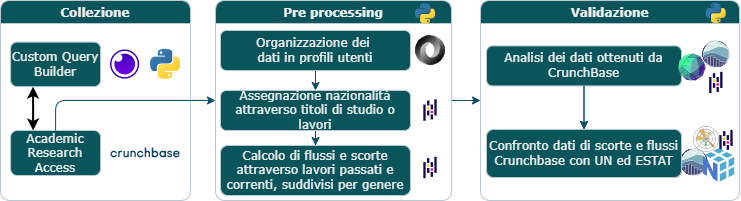
\includegraphics[width=1\textwidth]{images/SVG/diagram2.png}
    \caption{Diagramma della metodologia}
    \label{fig:digram}
\end{figure}

Come mostrato in Figura \ref{fig:digram}, la metodologia proposta è divisa in tre fasi: collezione, pre-processing e validazione dei dati. 
La collezione dei dati è stata effettuata attraverso due diversi metodi: 
\begin{itemize}
    \item Custom Query Builder
    \item Crunchbase Academic Research Access
\end{itemize}
Il Custom Query Builder è stato utilizzato per la raccolta dei dati fino a che non è stata ottenuta la possibilità di accedere ai dati tramite Academic Research Access. 
I dati collezionati da Crunchbase seguendo l'approccio descritto in Sezione \ref{academic_access_section}, sono preprocessati al fine di estrapolare le informazioni relative agli utenti, ai flussi e alle scorte migratorie. 
Dopo la collezione e il preprocessing, è stata affrontata la validazione dei dati. Con questo obiettivo, le scorte ed i flussi calcolati a partire dai dati collezionati da Crunchbase sono stati confrontati con quelli nel MIMI mediante un analisi di correlazione.
Inoltre, i risultati sono stati visualizzati mediante 
\textit{chord diagram}\footnote{Il chord diagram, in italiano, diagramma a corda rappresenta i flussi e le connessioni tra diverse entità, chiamate nodi. Ciascuna entità è rappresentata da un segmento del perimetro circolare. Gli archi sono tracciati tra entità connesse. Inoltre, la dimensione dell'arco è proporzionale all'importanza o dimensione dell'entità misurata (scorte o flussi) \footnote{(From Data to Viz: Chord Diagram \url{https://www.data-to-viz.com/graph/chord.html}.}}, seguendo diversi livelli di aggregazione geografica.

\section{Collezione dei dati}
\label{sezionecollezionedati}
La collezione dei dati è avvenuta attraverso due metodi: il Custom Query Builder e l'Academic Research Access. Il Custom Query Builder è stato realizzato mediante lo studio del meccanismo di \textit{query} offerto dalla piattaforma Crunchbase. In un secondo momento è stato ottenuto l'accesso accademico ai dati che ha permesso di prelevare i dati ufficiali da Crunchbase.

Per determinare la validità dei dati ottenuti si confrontano con i dati del MIMI dataset, per scorte e flussi. Ogni confronto con i dati ufficiali consiste nel calcolo della correlazione e la visualizzazione dei dati su grafici di dispersione. 

\subsection{Query Builder}
\label{sottosezionequerybuilder}
Per ottenere i dati si è scelto, nella fase iniziale, di sfruttare il Query Builder offerto dalla piattaforma Crunchbase.
Il Query Builder permette di filtrare in base alle entità, tra cui persone, compagnie, investitori, acquisizioni.
Dato che l'obiettivo di questa tesi è studiare la migrazione delle persone altamente specializzate abbiamo limitato la collezione dei dati alle persone.
Il Query Builder permette di filtrare ulteriormente la ricerca sulla base di varie informazioni degli utenti, tra cui la carriera lavorativa, i titoli di studio, eventi ai quali hanno partecipato e il genere.

Una volta eseguita una ricerca tramite il Query Builder, il sito pubblico di Crunchbase  restituisce i primi 5 profili che soddisfano la query più il numero totale di profili. Il nostro approccio non utilizza i profili individuali, ma salva solamente il numero totale di profili, che saranno interpretati come la dimensione delle scorte e flussi migratori. Questo approccio rispetta la privacy degli utenti e risulta in numeri aggregati e anonimizzati. 


Per studiare la migrazione abbiamo costruito dei query che selezionano i soli profili utenti di persone che hanno conseguito la laurea in un set di paesi selezionati\footnote{Stati Uniti, Canada, India, Filippine, Pakistan, Australia, Cina, Singapore, Brasile, Giappone e continente europeo.} (lo stato di laurea sarà considerato un proxy per la nazionalità). Per ottenere le scorte annuali è stato estratto il numero di persone che lavoravano il 1° Gennaio di ogni anno, dal 2010 al 2020, in ciascuno degli stati selezionati. 
Infine, per ottenere i flussi, è stato estratto il numero di persone che hanno cambiato impiego durante ciascun anno, dal 2010 al 2020, sposandosi tra gli stati selezionati. 


Al fine di automatizzare il processo di collezione abbiamo deciso di applicare tecniche di \textit{reverse engineering}\footnote{Ingegneria/ingegnerizzazione inversa.}. 
Grazie alla comprensione del meccanismo di comunicazione del sito è stato realizzato il Custom Query Builder (Sezione \ref{customquerybuilder}), che genera automaticamente le richieste da inviare, le invia e ne gestisce le risposte.

\subsubsection{Custom Query Builder}
\label{customquerybuilder}
Per realizzare un programma che interagisse in modo diretto con i server di Crunchbase, è stato analizzato il codice html del sito web. Questo ha permesso di comprendere la fonte dei dati rappresentati sulla piattaforma web. L'analisi ha portato a comprendere che Crunchbase sfrutta un API interna, con richieste/risposte JSON via http per il trasferimento dati.
Il Codice \ref{lst:querybuilderjsonquery} mostra la struttura delle le richieste. 
Sulla base di questa struttura di esempio, è possibile realizzare una lista di query personalizzata. 
Le query essendo trasferimenti di tipo http necessitano di un header; nel nostro caso la copia dell'header generato dal browser.
L'header contiene informazioni, tra cui quelle relative ai linguaggi accettati con il relativo ordine di preferenza (nel nostro caso \texttt{it-IT,it;q=0.9,en-US;q=0.8,en;q=0.7}), al tipo di contenuti accettati e inviati (nel nostro caso \texttt{application/json} e \texttt{text/plain}) e se c'è già stato un collegamento vi saranno dei cookie\footnote{Piccoli file generati dai siti web salvati nella memoria del computer dell'utente, per mantenere informazioni sulle connessioni 
effettuate in precedenza.}. 

La codifica in Python delle richieste è stata generata dal software Insomnia\footnote{Insomnia: \url{https://github.com/Kong/insomnia}.}.
Insomnia permette di trasformare in codice Python le richieste http come quella nel Codice \ref{lst:querybuilderjsonquery}, previa estrazione delle richieste inviate nel browser. 
Nonostante l'utilizzo di Insomnia, la richiesta deve essere comunque adattata per ogni singola query.Inoltre, dopo un certo numero di richieste il sito di Crunchbase richiede un captcha, che nel nostro caso abbiamo eseguito manualmente. Questa procedura è abbastanza scalabile per la quantità di richieste che abbiamo dovuto eseguire per questa analisi.


\usemintedstyle{rainbow_dash, escapeinside=||, fontfamily = courier, baselinestretch=1, fontsize=\footnotesize, linenos=true, autogobble}

\begin{listing}
\begin{minted}{json}
{
  "query": [                
    { 
      "type": "sub_query",   |\label{first_subquery}|
      "collection_id": "organization.has_alumni.reverse",
      "query": [
        {
          "field_id": "location_identifiers", 
          "operator_id": "includes",
          "values": ["9dd7a8c5-7b7f-7785-90f4-fed17fa5a6ff"]  |\label{uni_location}|
        }
      ] |\label{first_subquery_end}|
    }, 
    { 
      "type": "sub_query", |\label{second_subquery}|
      "collection_id": "job.has_past_job.forward",
      "query": [
        {
          "type": "sub_query", 
          "collection_id": "organization.has_past_position.reverse",
          "query": [
            {
              "field_id": "location_identifiers", 
              "operator_id": "includes",
              "values": ["f110fca2-1055-99f6-996d-011c198b3928"] |\label{dest_location}|
            }
          ]
        },
        { |\label{date}|
          "field_id": "started_on", "operator_id": "lte", 
          "values": ["1/1/2010"] 
        },
        {
          "field_id": "ended_on", "operator_id": "gte", 
          "values": ["1/1/2010"]
        } |\label{date_end}|
      ]
    } |\label{second_subquery_end}|
  ]
}
\end{minted}
\caption{Esempio di codice JSON delle richieste che il Query Builder invia ai propri server}
\label{lst:querybuilderjsonquery}
\end{listing}
%%


Il Codice JSON in \ref{lst:querybuilderjsonquery} è parte di una query tipica che Crunchbase invia ai propri server per richiedere le scorte migratorie di nazionalità italiana negli Stati Uniti d'America per il 2010. La prima porzione della query (righe \ref{first_subquery} - \ref{first_subquery_end}) filtra le persone che hanno studiato in un istituto la cui posizione è in Italia (riga \ref{uni_location}).
La seconda parte della query (righe \ref{second_subquery} - \ref{second_subquery_end}) impone che i lavori effettuati dalle  persone filtrate dalla prima sub query (righe \ref{first_subquery} - \ref{first_subquery_end}) siano per aziende negli Stati Uniti d'America (riga \ref{dest_location}). Inoltre, ogni rapporto lavorativo deve essere iniziato prima e  terminato dopo il 1° Gennaio 2010 (righe \ref{date} - \ref{date_end}). 


Crunchbase rappresenta ogni stato attraverso un codice UUID\footnote{Universally Unique Identifier, in italiano identificativo univoco universale.}. Di conseguenza, è stata realizzata manualmente una lista delle coppie Stato-UUID analizzando il codice html dei luoghi suggeriti nella pagina di compilazione della query.

%% CODICE CHE GENERATE LE QUERY RELATIVE AGLI STOCK 
\begin{listing}[htbp]
\begin{minted}{Python}
def queries_lite_create():
    Countries = countries_get("SUBSET COUNTRIES")  # Coppie Stato_UUID |\label{lista_uuid}|
    QUERIES = read_json("queries_lite")            # Carico le query  |\label{lista_querydainviare}|
    combination = product(Countries, repeat=2)     # Permutazioni di stati |\label{combinazionestati}|
    for combo in combination:  |\label{ql_for_start}|
        if combo[0] not in QUERIES:     # Se la combinazione non è
            QUERIES[combo[0]] = {}      # presente la aggiungo
        if combo[1] not in QUERIES[combo[0]]:   
            QUERIES[combo[0]][combo[1]] = {}
        for YEAR in range(2010, 2022):                      
            QUERIES[combo[0]][combo[1]][str(YEAR)] = {}
            for gender in {"male", "female"}:
                payload = payload_update_lite( |\label{ql_create}|
                    Countries[combo[0]]["uuid"],
                    Countries[combo[1]]["uuid"],
                    YEAR,
                    gender
                )
                QUERIES[combo[0]][combo[1]][str(YEAR)][gender] = []
                QUERIES[combo[0]][combo[1]][str(YEAR)][gender].append(payload)  |\label{ql_append}|
    |\label{ql_for_end}|
    write_json(QUERIES, "queries_lite.json")    # Scrivo le nuove query |\label{salvo_query_generate}|
                                                # calcolate nel file JSON
                                                # delle query
\end{minted}
\caption{Funzione \texttt{queries\_lite\_create()} che genera un file JSON contenente le query relative alle scorte migratorie da inviare a Crunchbase}     \label{lst:stockquerygen}
\end{listing}
\par
La Funzione \texttt{queries\_lite\_create()} nel Codice \ref{lst:stockquerygen}, realizza un documento in formato JSON (riga \ref{salvo_query_generate}) che contiene tutte le query relative alle scorte migratorie che, successivamente, saranno inviate a Crunchbase. Utilizza la libreria \texttt{json} per la serializzazione e la de serializzazione dei dati (righe \ref{lista_uuid}, \ref{lista_querydainviare}, \ref{salvo_query_generate}) e la funzione \texttt{product} della libreria Itertools (riga \ref{combinazionestati}) per generare un insieme di combinazioni di ordine 2 degli stati selezionati. 
All'interno del ciclo \texttt{for} (righe \ref{ql_for_start} - \ref{ql_for_end}) vengono generate le query ed aggiunte alla struttura in locale (righe \ref{ql_create}, \ref{ql_append}).

%% CODICE CHE INVIA LE QUERY RELATIVE AGLI STOCK GENERATE DALL'ALGORITMO PRECEDENTE 
\begin{listing}[htbp]
\begin{minted}{python}
def send_queries():
    dataset = functions.read_json("SavedCountries_lite") |\label{read_json}|
    link = "/v4/data/searches/people?source=custom_query_builder"
    ed_country, work_country, year, \
    gender, query, queries = functions.get_query_lite(dataset)
    
    while ed_country and work_country and year and \ 
    gender and query and queries: |\label{ciclosendquery}|
        try:
            conn.request("POST",   |\label{richiestasendquery}|
                link, 
                query, 
                new_header())
                
            res = conn.getresponse()
            data = json.loads(res.read())["count"]
        except:
            print("Request Error")
            return
            
        if ed_country not in dataset:
            dataset[ed_country] = {}
        if work_country not in dataset[ed_country]:
            dataset[ed_country][work_country] = {}
        if year not in dataset[ed_country][work_country]:
            dataset[ed_country][work_country][year] = {}
        
        dataset[ed_country][work_country][year].update({gender: data})
        
        functions.write_json(dataset, "SavedCountries_lite.json")
        functions.write_json(queries, "queries_lite.json") |\label{salvaquerysudisco}|
        
        time.sleep(random.randint(8, 12))
        ed_country, work_country, year, \ 
        gender, query, queries = functions.get_query_lite(dataset) |\label{getnewquery}|
    |\label{ciclosendquery_end}|
\end{minted}
\caption{Funzione \texttt{send\_queries()} per l'invio delle query.}
\label{lst:stockquerysend}
\end{listing}

La Funzione \texttt{send\_queries()} nel Codice \ref{lst:stockquerysend} invia le query contenute nel file creato dalla Funzione \texttt{queries\_lite\_create()} nel Codice \ref{lst:stockquerygen}. 
Genera un file di tipo JSON con la struttura del Codice \ref{lst:stock_data}, contenente il risultato ricevuto dai server di Crunchbase (riga \ref{salvaquerysudisco}) aggiornandolo di volta in volta con il risultato della nuova query eseguita (righe  \ref{richiestasendquery}, \ref{getnewquery}) nel ciclo \texttt{while} (righe \ref{ciclosendquery} - \ref{ciclosendquery_end}).
Il Codice JSON \ref{lst:stock_data} contiene la provenienza delle scorte (riga \ref{natline}) riferite ad un determinato paese (riga \ref{destline}). Si ha poi un esempio di alcuni anni a cui si riferiscono le scorte suddivise per genere (righe \ref{yearline}, \ref{yearline_end}). 

%% RISULTATO TIPO DELLA FUNZIONE CHE GESTISCE L'INVIO E LE RISPOSTE
\begin{listing}[htbp]
\begin{minted}{json}
{
    "China": {              |\label{natline}|
        "China": {          |\label{destline}|
            "2021": {      |\label{yearline}|
                "female": 0,
                "male": 0
            },
            "2010": {
                "female": 39,
                "male": 176
            },
            "2011": {
                "female": 36,
                "male": 155
            }             |\label{yearline_end}|
        }
    }
}
\end{minted}
\caption{Codice JSON di esempio delle scorte}
\label{lst:stock_data}
\end{listing}


Il metodo proposto ha permesso di ottenere tutte le scorte migratorie separate per nazionalità, residenza, anno e genere per i paesi selezionati.
In termini di tempo, ottenere le risposte per tutte le scorte ha richiesto \(\simeq 11\) ore, incluso il tempo necessario per generare e cambiare l'header quando non era più valido.

%I flussi sono stati calcolati direttamente attraverso l'accesso accademico ai dati Crunchbase (Sezione \ref{preprocessing}), è stato comunque implementato nel Custom Query Builder il codice per la richiesta dei flussi.

Il Custom Query Builder ha delle limitazioni, la più importante di queste è il fatto che i filtri nelle query (Sezione \ref{customquerybuilder}) devono valere sempre tutti. Quindi il Custom Query Builder conta le persone varie volte, una per ogni città in cui hanno studiato. Inoltre, considera i generi maschili e femminili, ma gli utenti possono scegliere di non menzionare il genere portando il Custom Query Builder ad ignorarli nelle richieste.

%Questo porta ad avere molti dati sovrastimati. Ad esempio un periodo di studio all'estero risulterà come cittadinanza per un quell'utente, e così via per ogni suo titolo di studio. 

\subsection{Crunchbase Academic Research Access}
\label{academic_access_section}
L'accesso all'API accademica di Crunchbase è possibile sottomettendo una domanda a Crunchbase che viene accettata dall'azienda dopo una valutazione del progetto e un colloquio. Una volta ottenuto l'accesso si possono inviare richieste ai server Crunchbase. Le richieste inviabili attraverso l'API condividono in parte la struttura di quelle nel Codice \ref{lst:querybuilderjsonquery}, così come alcune limitazioni (Sezione \ref{customquerybuilder}).
Tuttavia, l'accesso all'API accademica consente di scaricare in locale tutte le entità più significative del sito.

Tra le entità a disposizione\footnote{Documentazione di Crunchbase: \url{https://data.crunchbase.com/docs/daily-csv-export}.} ci focalizziamo sulle organizzazioni (\textit{organizations}), i titoli (\textit{degrees}), i lavori (\textit{jobs}) e le persone (\textit{people}). L'entità \textit{degrees} è costituita dai titoli acquisiti da un utente presso una determinata sede. L'entità \textit{jobs} è costituita invece dai lavori presenti e passati di un utente preso determinate organizzazioni. 
La struttura dei dati è organizzata in diversi file csv, similmente alle tabelle di un database relazionale. Ogni file rappresenta un tipo di entità con i propri attributi come chiave primaria, chiavi referenziate e le informazioni relative ad un elemento dell'entità come la posizione.


Questi dati sono stati usati per calcolare le scorte di migranti e i flussi migratori. 

Le informazioni ottenute sono state organizzate in file JSON dove, per ogni utente è presente la posizione dichiarata, il genere, la lista dei lavori effettuati con informazioni relative al luogo e al periodo di lavoro e lista dei diplomi ottenuti con relativa posizione.


\begin{listing}[htbp]
\begin{minted}{Python}
def totalCreate( bulk_dir=None, save=False):
    
    all_people = people_parsing(bulk_dir=bulk_dir)  |\label{ppl_parser}|
    activities = organization_parsing(bulk_dir=bulk_dir)
    jobs = jobs_parsing(all_people=all_people,
            activities=activities, bulk_dir=bulk_dir)
    degrees = degree_parsing(all_people=all_people, 
            activities=activities, bulk_dir=bulk_dir) |\label{deg_parser}|
    # COMMON STRINGS
    p_loc = "person_location"
    p_gen = "person_gender"
    jperson_uuid = "job_person_uuid"
    dperson_uuid = "person_degree_uuid"
    
    my_persona_db = {}
    with alive_bar(len(jobs) + len(degrees), title="Total", \ 
        force_tty=True, spinner="classic") as Total_bar: |\label{totalbar_declaration}|
        
        for each in jobs: |\label{job_for_total}|
            if jobs[each][jperson_uuid] not in my_persona_db:
                my_persona_db[jobs[each][jperson_uuid]] = {
                    p_gen: jobs[each][p_gen],
                    p_loc: jobs[each][p_loc],
                    'jobs': [],
                    'degrees': []
                }
            jobp = jobs[each]   
            my_persona_db[jobp[jperson_uuid]]['jobs'].append(jobp)|\label{job_total_get}|  
            Total_bar() |\label{totalbar_progress1}|
        |\label{job_for_total_end}|
    
        for each_deg in degrees: |\label{deg_for_total}|
            if degrees[each_deg][dperson_uuid] not in my_persona_db:
                my_persona_db[degrees[each_deg][dperson_uuid]] = {
                    p_gen: degrees[each_deg][p_gen],
                    p_loc: degrees[each_deg][p_loc],
                    'jobs': [],
                    'degrees': []
                }
            degp = degrees[each_deg]
            my_persona_db[degp[dperson_uuid]]['degrees'].append(degp)|\label{deg_total_get}|  
            Total_bar() |\label{totalbar_progress2}|
        |\label{deg_for_total_end}|

    if save: |\label{save_par}|
        with open("Crunchbase Data/total.json", "w+") as outFile:
            outFile.write(json.dumps(my_persona_db, indent=4))
    return my_persona_db |\label{ret_line}|
\end{minted}
\caption{Funzione che genera la struttura degli utenti con relative informazioni}
\label{lst:tot_create}
\end{listing}

La Funzione \texttt{totalCreate()} nel Codice \ref{lst:tot_create} si occupa di organizzare i dati nella struttura JSON descritta nel Codice \ref{lst:json_fromARA}. Vengono caricati i dati dalle quattro entità interessate (righe \ref{ppl_parser} - \ref{deg_parser}). Attraverso un ciclo \texttt{for} (righe \ref{job_for_total} - \ref{job_for_total_end}) vengono prese le informazioni relative ai lavori e vengono memorizzate in una struttura locale (righe \ref{job_total_get}). Lo stesso processo viene applicato per i titoli di studio (righe \ref{deg_for_total} - \ref{deg_for_total_end}). Viene utilizzata una barra di progresso per visualizzare lo stato del processo (righe \ref{totalbar_declaration}, \ref{totalbar_progress1}, \ref{totalbar_progress2}). 
Infine, se si passa il parametro \texttt{save} (riga \ref{save_par}) vero, verrà serializzato tutto il contenuto della struttura realizzata in locale. Viene in ogni caso restituita al chiamante tutta la struttura (riga \ref{ret_line}).


\begin{listing}[htbp]
\begin{minted}{json}
{
    "person_UUID": {                                            |\label{persUUID}|
        "person_gender": "male",                                |\label{persGenU}|
        "person_location": "USA",                               |\label{persStateU}|
        "jobs": [                                               |\label{jobslist}|
            {
                "job_organization_uuid": "ORG_UUID",
                "job_start_date": "2005-10-01",
                "job_end_date": "2014-06-01",
                "job_is_current": false,
                "job_location": "USA"
            },
            {
                "job_organization_uuid": "ORG_UUID",
                "job_start_date": "2001-01-01",
                "job_end_date": "2002-01-01",
                "job_is_current": false,
                "job_location": "GBR"
            }
        ],                                                      |\label{jobslist_end}|
        "degrees": [                                            |\label{degslist}|
            {
                "university_degree_uuid": "UNI_UUID",
                "degree_completed": true,
                "university_location": "USA"
            }
        ]                                                       |\label{degslist_end}|
    },
}
\end{minted} 
\caption{Codice JSON di esempio per un utente}
\label{lst:json_fromARA}
\end{listing}

Il Codice \ref{lst:json_fromARA} rappresenta l'esempio di come vengono organizzate le informazioni relative ad un utente, nella struttura generata dalla Funzione \texttt{totalCreate()} nel Codice \ref{lst:tot_create}. Per ogni utente, rappresentato dal suo \textit{UUID} (riga  \ref{persUUID}), si ha il suo genere (riga \ref{persGenU}), la location che dichiara (riga \ref{persStateU}), la lista dei lavori (righe \ref{jobslist} - \ref{jobslist_end}) e dei titoli di studio (righe \ref{degslist} - \ref{degslist_end}).


%****************************************
\section{Preprocessing ed estrazione delle informazioni}
\label{preprocessing}
\begin{figure}[ht]
    \begin{subfigure}{\textwidth}
        \centering
        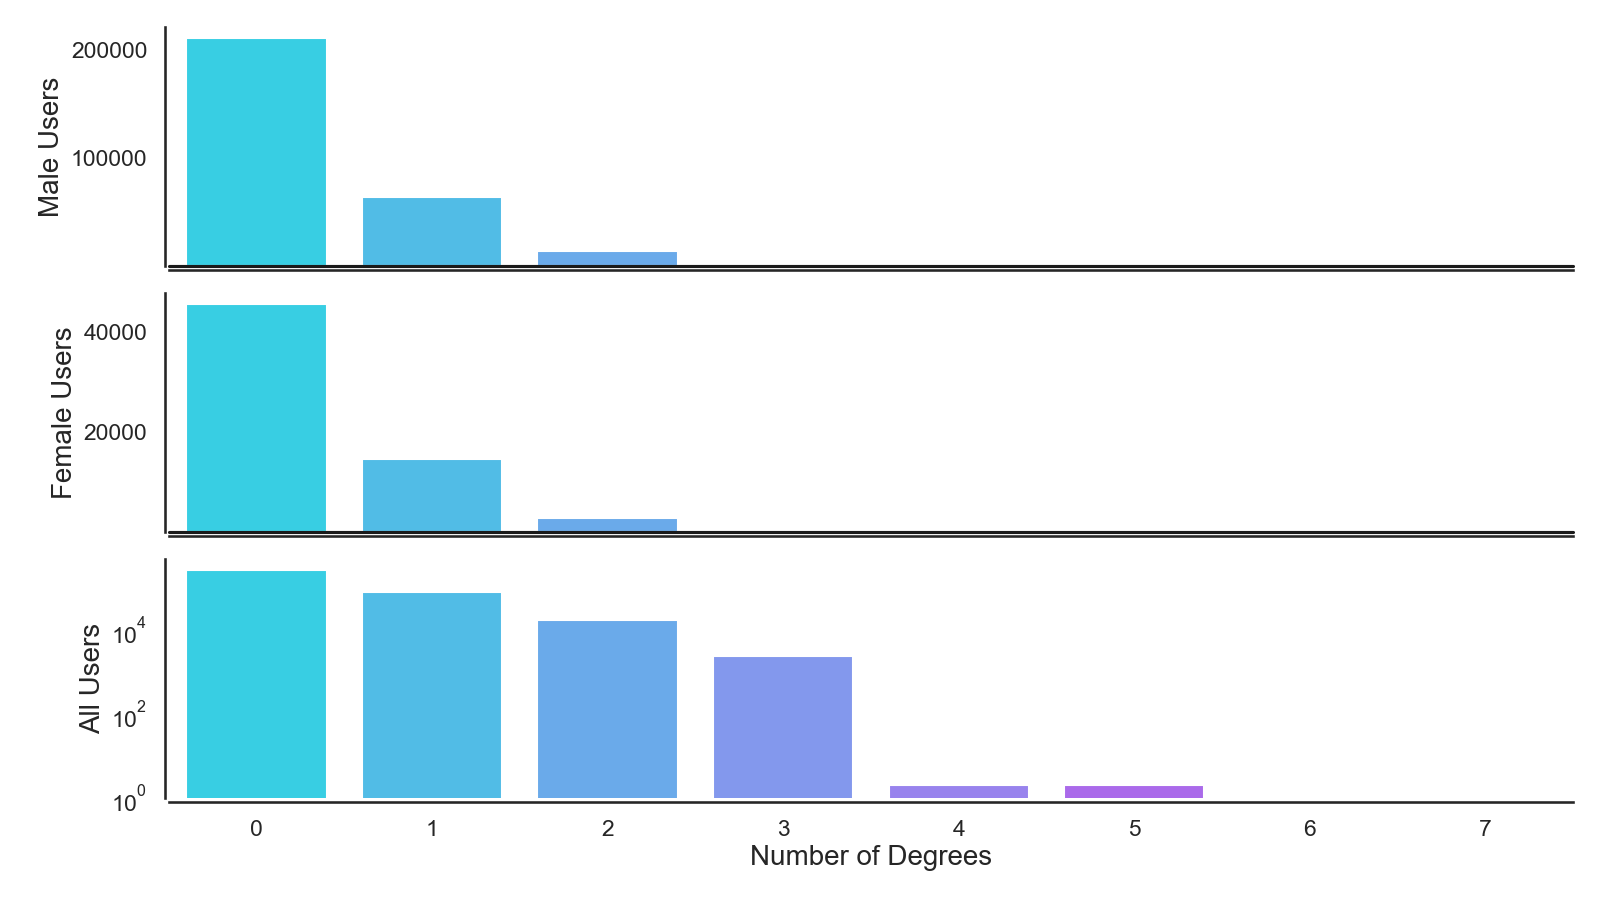
\includegraphics[width=\textwidth]{images/histogram/degrees_histogram.png}
        \caption{Istogramma dei titoli di studio}
        \label{fig:degreesbarplot}
    \end{subfigure}
\end{figure}
\begin{figure}[tb]\ContinuedFloat
    \begin{subfigure}{\textwidth}
        \centering
        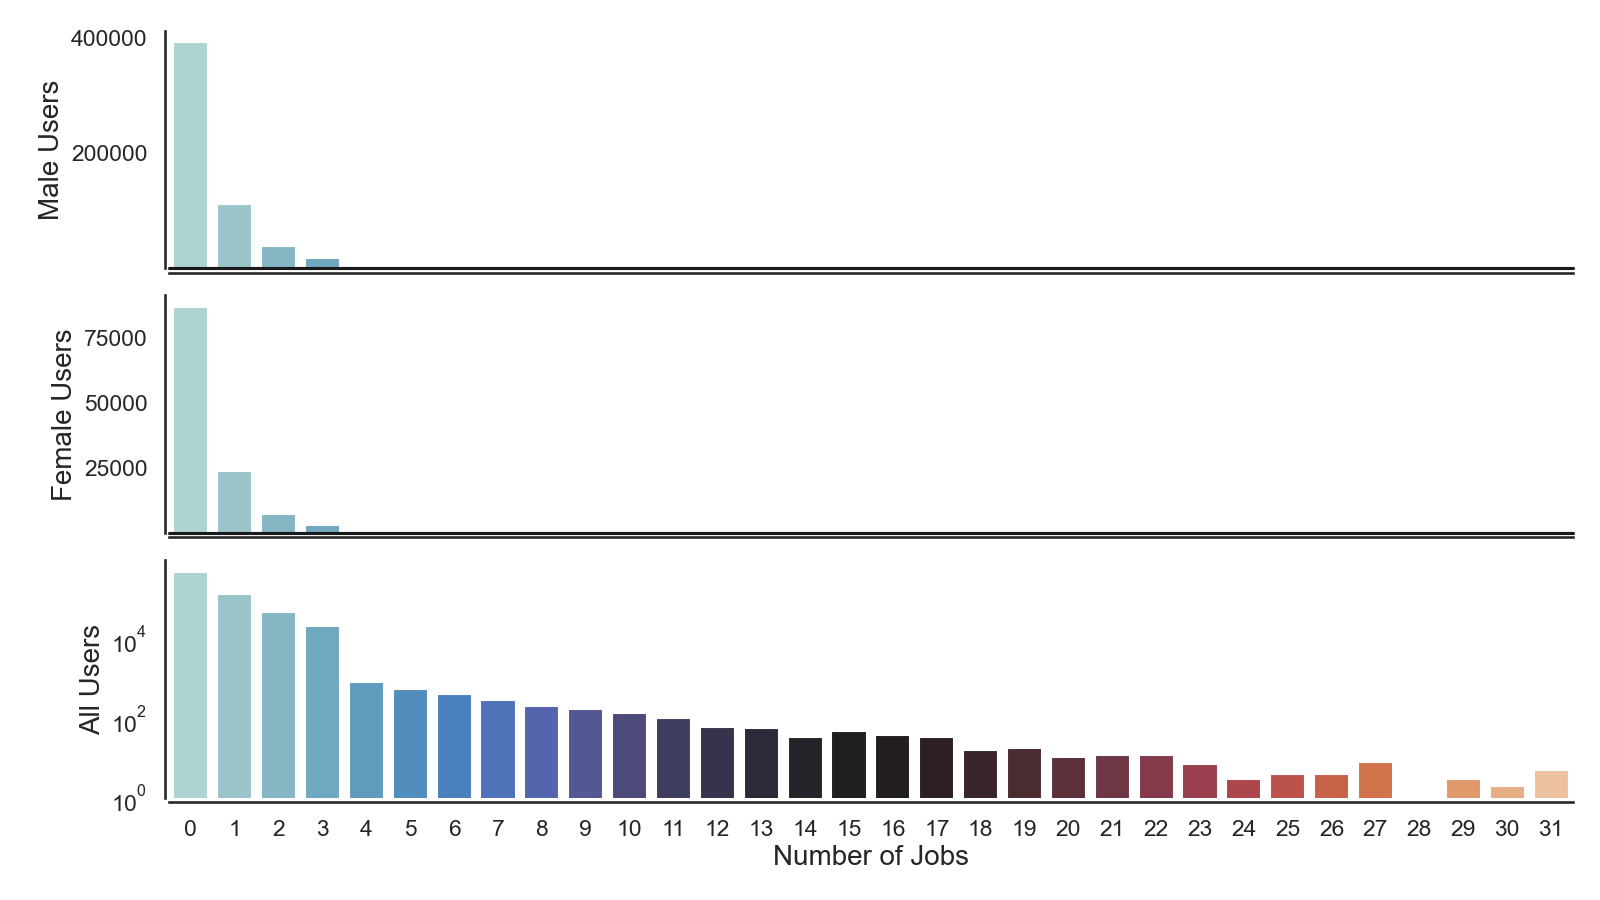
\includegraphics[width=\textwidth]{images/histogram/jobs_histogram.png}
        \caption{Istogramma dei lavori}
        \label{fig:jobsbarplot}
    \end{subfigure}
\end{figure}
La fase di \textit{preprocessig} ed estrazione delle scorte e dei flussi dai dati Crunchbase, ha avuto fondamento grazie un'analisi degli utenti Crunchbase. Questa ha determinato quale fosse la distribuzione dei titoli di studio e dei lavori sulla piattaforma. 
Il grafico in Figura \ref{fig:degreesbarplot} mostra che la maggior parte degli utenti ha tra uno e tre titoli di studio. 
Dalla Figura \ref{fig:jobsbarplot} si nota che maggior parte degli utenti ha avuto/ha almeno un lavoro.

Abbiamo definito la ``nazionalità'' come il paese più ricorrente tra le posizioni delle istituzioni presso le quali la persona ha ottenuto titoli di studio\footnote{A parità di numeri viene considerato il titolo di studio conseguito meno di recente.}. Se la nazionalità non è deducibile dai titoli di studio, ad esempio per mancanza della localizzazione delle istituzioni, si utilizza la posizione dell'azienda per cui l'utente ha lavorato meno di recente. 
La ''residenza'' è stata invece dedotta dai trasferimenti lavorativi degli utenti, definendola attraverso la posizione dell'azienda con la quale l'utente ha terminato il rapporto lavorativo.
\FloatBarrier
\begin{listing}[htbp]
\begin{minted}{Python}
def extractStocks(total=None, save=False, counter=0):
    my_db = NestedDict()
    if total is None:               |\label{caricatotalfile}| 
        total = read_total()
    if counter == 0:
        counter = count_jobs(total)
    with alive_bar(counter, title="Stocks", 
                   force_tty=True, spinner="classic") as stocks_bar:

        for person in total:        |\label{person_for_loop}| 
            ed_country := get_nationality(total[person]['degrees'], 
                                          total[person]['jobs'])
            if not len(total[person]['jobs']) or 
               not ed_country): |\label{checkifhavejobsgetNat}|
                continue
                
            for person_job in total[person]['jobs']:  |\label{person_jobs_for_loop}| 
                stocks_bar()
                if math.isnan(float(person_job['job_location'])) or 
                   math.isnan(float(person_job['job_start_date'])):     |\label{check_job_loc_date}|
                    continue
                    
                job_loc = person_job['job_location']
                job_start = dt.strptime(person_job['job_start_date'], 
                                            "%Y-%m-%d")
                if math.isnan(float(person_job['job_end_date'])):
                    if person_job['job_is_current']:
                        job_end = dt.strptime(2023, "%Y")
                    else:
                        continue
                else:
                    job_end = dt.strptime(person_job['job_end_date'],   |\label{check_job_loc_date_end}|
                                                      "%Y/%m/%d")
                                                      
                for year in range(2010, 2021):
                    year_t = dt.strptime(str(year), "%Y")
                    if year_t < job_start or year_t > job_end:
                        continue
    
                    gender = genderPrs(total[person]['person_gender'])   
                    my_db[ed_country][job_loc][str(year)][gender] += 1 |\label{stockSumLine}|
                |\label{person_jobs_for_loop_end}| 
        |\label{person_for_loop_end}| 
    if save:
        fileName = "Crunchbase Query Results/query_stocks_results.json"
        stockFile = open(fileName, "w+")
        stockFile.write(json.dumps(my_db, indent=4))
    return my_db
\end{minted}
\caption{Codice per l'estrazione delle scorte}
\label{lst:stockget}
\end{listing}

La Funzione \texttt{extractStocks(total=None, save=False, counter=0)} nel Codice \ref{lst:stockget} scorre i profili utente che possono essere passati in forma di dizionario oppure vengono caricati dalla memoria se presenti (riga \ref{caricatotalfile})). 
Per ogni utente si controlla che abbia avuto un impiego lavorativo e si estrapola la nazionalità dai titoli di studio (riga \ref{checkifhavejobsgetNat}). Successivamente si scorre la lista dei suoi lavori (righe \ref{person_jobs_for_loop} - \ref{person_jobs_for_loop_end}), e in questo ciclo si ottengono la posizione dell'azienda in cui ha lavorato e le date relative al rapporto lavorativo (righe \ref{check_job_loc_date} - \ref{check_job_loc_date_end}). Infine, si incrementano i valori delle scorte (in locale) in base ai dati che vengono incontrati (riga \ref{stockSumLine}). Come la Funzione \texttt{totalCreate()} nel Codice \ref{lst:tot_create}, anche questa permette di usare il parametro \texttt{save} per salvare il risultato; in ogni caso restituisce al chiamante le scorte calcolate.

Il preprocessig dei flussi viene effettuato mediante un processo identico a quello della Funzione \texttt{extactStocks()} nel Codice \ref{lst:stockget}, con un ciclo in più all'interno del ciclo dei lavori (righe \ref{person_jobs_for_loop} - \ref{person_jobs_for_loop_end}) per scorrere gli altri lavori dell'utente e confrontarne il periodo d'inizio e fine. Questo permette di stabilire se durante un determinato anno l'utente ha cambiato residenza.

\begin{listing}[htbp]
\begin{minted}{json}
{
    "USA": {    |\label{natState1}|
        "USA": {        |\label{destState1}|
            "2010": {   |\label{year1}|
                "male": 22,
                "female": 511082,
                "unknown": 1
            },          |\label{year1_end}|
        },
        "ITA": {        |\label{destState2}|
            "2015": {   |\label{year2}|
                "male": 0,
                "female": 11,
                "unknown": 0
            },
            "2016": {...}   |\label{year2_end}|
        },
    },
    "CAN": {...} |\label{natState2}|
}
\end{minted}
\caption{Codice di esempio scorte Academic Research Access}
\label{lst:stocksARA}
\end{listing}

Il metodo proposto ha premesso di ottenere le scorte di migranti organizzate nella medesima struttura di quelle nel MIMI dataset. Un esempio è mostrato nel Codice \ref{lst:stocksARA}. Il primo stato (e.g. righe \ref{natState1}, \ref{natState2}) indica la nazionalità delle scorte, il secondo (e.g. righe \ref{destState1}, \ref{destState2}) indica il paese in cui sono state conteggiate. Per ogni coppia si ha poi la lista degli anni con i relativi valori suddivisi per genere (righe \ref{year1}-\ref{year1_end}, \ref{year2}-\ref{year2_end}). 



\begin{listing}[htbp]
\begin{minted}{Python}
def common_items(d1, d2):
    return {k: common_items(d1[k], d2[k]) 
    if (k not in ["2010", "2015", "2020"]) and isinstance(d1[k], dict) |\label{istanceofdict}|
    else {'Crunchbase': sum(d1[k][e] for e in d1[k]), 
          'UN': int(d2[k]['total'])}
        for k in (d1.keys() & d2.keys())}   |\label{forallkey}| 
\end{minted}
\caption{Codice che interseca due dict}
\label{lst:dictIntersect}
\begin{minted}{Python}
def stocksIntersection(natStateFilter=None, stockStateFilter=None,
                       natContinentFilter=None, stockContinentFilter=None):
    cont = {}
    if natContinentFilter or stockContinentFilter:
        cont = dataextractor.read_json("Countries/ENA.json")
    stocks_query_file = "CrunchQR\stocks_results_with_jobs.json"
    un_stocks_file = "MIMI\Stocks\\UN_stocks.json"

    UN = dataextractor.read_json(un_stocks_file)                |\label{unstocksData}|
    crunchbase = dataextractor.read_json(stocks_query_file)     |\label{cbstockData}|
    result = common_items(crunchbase, UN)   |\label{dictintersections}|

    my_db = []
    for entry in result:            |\label{stockIntersectFor}|
        if (natContinentFilter and entry not in cont[natContinentFilter]) or \
                natStateFilter and entry != natStateFilter:
            continue
        for dest in result[entry]:
            if (stockContinentFilter and dest not in cont[stockContinentFilter]) or \
                    stockStateFilter and dest != stockStateFilter:
                continue
            for year in result[entry][dest]:
                my_db.append({'Origin': entry, 'Destination': dest, 'Year': year,
                              'Crunchbase': result[entry][dest][year]['Crunchbase'],
                              'UN': result[entry][dest][year]['UN']})
    |\label{stockIntersectFor_end}|

    df = pd.DataFrame(my_db)        |\label{dictToDataframe}|
    return df                       |\label{dictRetStocksIntersect}|
\end{minted}
\caption{Codice che interseca le scorte ufficiali con quelle Crunchbase}
\label{lst:stockIntersect}
\end{listing}


La Funzione ricorsiva \texttt{common\_items(d1, d2)} nel Codice \ref{lst:dictIntersect} effettua l'intersezione di due dict passati come parametro. Per ogni chiave k presente in entrambi i dizionari (\ref{forallkey}), se la chiave è istanza di dict viene richiamata ricorsivamente la funzione sui valori contenuto nei dizionari alla chiave k; altrimenti se la chiave è un numero compreso tra 2010, 2015 e 2020 (gli anni delle scorte in UN) viene ritornato il valore delle scorte presente in entrambi i dizionari. 
La Funzione \texttt{stockIntersection()} nel Codice \ref{lst:stockIntersect} carica i dati delle scorte (UN e Crunchbase) in locale (righe \ref{unstocksData}, \ref{cbstockData}). Se chiamata senza parametri restituisce il risultato della funzione \texttt{common\_items(d1, d2)} in un dataframe (righe \ref{dictintersections}, \ref{dictToDataframe}, \ref{dictRetStocksIntersect}). La Funzione \texttt{stockIntersection()} accetta quattro parametri come filtri: nazionalità, stato scorte, continente della nazionalità,  e continente delle scorte. Tutti i filtri vengono controllati all'interno del ciclo che scorre i dati ottenuti dall'intersezione di UN e Crunchbase (righe \ref{stockIntersectFor} - \ref{stockIntersectFor_end}). 


Il preprocessing descritto in questa sezione ha permesso di selezionare tutte le coppie di paesi (nazionalità - paese scorte) per cui sono presenti i dati sia nei dati ufficiali che in quelli Crunchbase. Ciò ha permesso di utilizzare i dati per la validazione delle scorte direttamente dalla struttura generata dalla Funzione \texttt{stockIntersection()} nel Codice \ref{lst:stockIntersect}. 

Per ottenere l'intersezione dei flussi Crunchbase con i flussi dei dati ufficiali è stato utilizzato un codice simile a quello per le scorte con un ciclo \texttt{for} ulteriore per scorre le residente degli utenti. Dato che per i flussi è stata usata la medesima struttura delle scorte, generata in fase di \textit{preprocessing} (Sezione \ref{preprocessing}). Con una leggera modifica che annida un ulteriore paese nel Codice Json \ref{lst:stocksARA} formando così una tripla cittadinanza-residenza-destinazione.

\section{Validazione dei flussi e scorte}
\label{analisidatiARA}
In questa sezione viene descritto il processo di validazione delle scorte e dei flussi collezionati da Crunchbase. 
Per visualizzare i dati migratori sono generati grafici di dispersione nei quali l'asse delle X rappresenta i dati di Crunchbase ottenuti mediante Academic Reseach Access e l'asse delle Y dai dati di confronto che possono essere dati Eurostat, UN o anche l'unione dei due. Ogni grafico presenta nella parte inferiore destra i valori delle correlazioni per validare i dati Crunchbase.  


\begin{listing}[htbp]
\begin{minted}{Python}
    df_matplot # ->> DATI INTERSECATI   |\label{intFunc}|
                    
    # GENERO TESTO CON TUTTE LE CORRELAZIONI
    string_on_plot = correlation_calc(df_matplot)  |\label{corrFunc}|

    # SCATTERPLOT
    p = sns.scatterplot()
    if stock: sns.regplot(x='Crunchbase',           |\label{trendLine}| 
                          y='Official', 
                          data=df_matplot)        
    plt.scatter(data=df_matplot,            |\label{scatterLine}| 
                x="Crunchbase", y="Official",        
                c="Crunchbase", cmap=color_map,
                edgecolors="black", linewidths=1, 
                alpha=0.6, s=100)                               |\label{scatterLine_end}|
    # RIGHT BAR
    cbar = plt.colorbar()
    
    # CORRELATIONS TEXT BOX                                 |\label{CorrAdd}|
    ob = offsetbox.AnchoredText(string_on_plot, loc="lower right", 
                                borderpad=2.5, prop=dict(size=15))
    ob.patch.set(boxstyle='round, pad=0.6')
    p.add_artist(ob)                                    |\label{CorrAdd_end}|
\end{minted}
\caption{Codice per realizzare i grafici di dispersione}
\label{lst:getScatter}
\end{listing}

Il Codice \ref{lst:getScatter} genera un grafico a dispersione con i valori Crunchbase sull'asse orizzontale e i valori dei dati ufficiali sull'asse verticale (righe \ref{scatterLine} - \ref{scatterLine_end}). Inoltre, solo per le scorte, genera una linea che indica la tendenza che hanno i valori delle scorte (riga \ref{trendLine}). Infine, aggiunge il riquadro delle correlazioni al grafico (righe \ref{CorrAdd} - \ref{CorrAdd_end}). La correlazione viene calcolata dalla Funzione \texttt{correlation\_calc()} (Codice \ref{lst:corrCalc}).


\begin{listing}[htbp]
\begin{minted}{Python}
def correlation_calc(df, source_="UN", flows=None):
    crunch = "Crunchbase"                                       |\label{confrCB}|
    source = source_                                            |\label{confrSource}|
    out = {}
    PearsLogOf = "PearsonLog" + source
    el = "_cit" if flows else ""                                |\label{citresFlows}|
    while True:                                                 |\label{whileFlows}|
        if df[crunch + el].any() and df[source + el].any():
            np.seterr(divide='ignore')
            
            # MASK INVALID VALUES
            maCruch = np.ma.masked_invalid(df[crunch + el])   |\label{crMask}|
            maOff = np.ma.masked_invalid(df[source + el])     |\label{ofMask}|
            logMaCruch = np.log(maCruch)   
            logMaOff = np.log(maOff)    
            
            # PEARSON CORR CALC                                 |\label{corrca}|
            out["Pearson" + el] = round(
                np.ma.corrcoef(maCruch, maOffDF)[0][1], 2)
            out["PearsonLog" + el] = round(
                np.ma.corrcoef(logMaCrunch, logMaOff)[0][1], 2)
            out[PearsLogOf + el] = round(
                np.ma.corrcoef(maCruch, logMaOff)[0][1], 2)
            out["PearsonLogCB" + el] = round(
                np.ma.corrcoef(logmaCrunch, maOffDF)[0][1], 2)

            # SPEARMAN CORR CALC
            df_corr_spearman = df.corr(method='spearman')
            out["Spearman" + el] = round(
                df_corr_spearman[crunch + el][source + el], 2)  |\label{corrca_end}|

            if flows:
                if el == "_cit":
                    el = "_res"
                    continue
            break

    # TO STRING
    if flows:
    new_d = "\n".join("{}: {!r}".format(k, out[k])
                      for k in sorted(out, key=len, reverse=False) 
                      if k.endswith("_cit"))
    new_d2 = "\n".join("{}: {!r}".format(k, out[k])
                       for k in sorted(out, key=len, reverse=False) 
                       if k.endswith("_res"))
    return new_d, new_d2

    return "\n".join("{}: {!r}".format(k, out[k])
                     for k in sorted(out, key=len, reverse=False))
\end{minted}
\caption{Codice per il calcolo delle correlazioni}
\label{lst:corrCalc}
\end{listing}
La Funzione \texttt{correlation\_calc()} nel Codice \ref{lst:corrCalc} genera una stringa contenente le correlazioni di Pearson e Spearman per i dati all'interno del dataframe, parametro della funzione. La funzione è strutturata per adattarsi al calcolo di correlazioni sia per stock che per flussi. Infatti, attraverso il parametro flows è possibile dire se il dataset passato si riferisce a flussi migratori (di default si calcolano le scorte).
Il Codice, per le scorte, si aspetta di trovare nel dataframe passato colonne con i nomi ''Crunchbase'' (riga \ref{confrCB}) e la stringa passata nel parametro source\_(riga \ref{confrSource}). 
Vengono mascherati i dati invalidi in entrambi i dataset con valori pari a 0 (righe \ref{crMask}, \ref{ofMask}), e successivamente vengono calcolare le varie correlazioni (righe \ref{corrca} - \ref{corrca_end}). Se il parametro flows è True, le colonne cercate nel dataframe saranno composte dal nome delle fonti (Crunchbase o fonte ufficiale) e da ''\_cit'' o ''\_res'' (riga \ref{citresFlows}), ed inoltre tutti i calcoli verranno eseguiti sia per i cittadini che per i residenti (riga \ref{whileFlows}).

La correlazione di Pearson ci dice se vi è una relazione lineare tra due variabili. Anche se il coefficiente di correlazione di Pearson indica che non ci sia correlazione lineare potrebbe esistere una relazione di altro tipo. Per questo motivo, i dati vengono sottoposti anche al calcolo del coefficiente di correlazione per ranghi di Spearman, che determina relazioni monotone. Quando i due indici sono vicini abbiamo una conferma della relazione


\section{Metodi e strumenti utilizzati}
\label{strumentiutilizzati}
Tutto il codice è stato scritto in Python e sviluppato utilizzando l'IDE PyCharm. E' stata utilizzata la versione \textit{education} fornita agli studenti dall'Università di Pisa, che ha svolto le operazioni di installazione delle librerie in modo automatico. 
Le librerie Python utilizzate riguardano:
\begin{itemize}
\item lettura di file JSON: json; 
\item manipolazione dei dati: dict, pandas\footnote{\url{https://pandas.pydata.org/docs/}}, alive-progress \cite{rsalmei} usata per determinare lo stato del processo;;
\item realizzazione di grafici: matplolib \cite{Hunter:2007}, seaborn \cite{Waskom2021}. Inoltre, plotapi\footnote{Plotapi: \url{https://plotapi.com/}} è stata usata per visualizzare in grafici circolari le scorte ed i flussi; 
\item calcolo delle correlazioni: NumPy \cite{harris2020array} per Pearson, e pandas per Spearman
\end{itemize}

%% Non è necessaria, momentaneamente
%\begin{comment}
\subsection{Correlazione}
L'Indice di correlazione è una misura che ci permette di stabilire quanto due insiemi di dati siano correlati, ovvero quanto i valori di uno dipendono dall'altro. 
I due indici di interesse per questo elaborato sono l'indice di Pearson per correlazioni lineari \cite{pearson} e l'indice di Spearman per correlazioni non lineari \cite{10.2307/2284441}. In questo elaborato abbiamo utilizzato l'indice di correlazione per validare i flussi e scorte migratorie estratte da Crunchbase.

\paragraph{Pearson}
Pearson impone alcune condizioni per i dati:
\begin{itemize}
\item Le due variabili devono essere entrambe di tipo quantitativo;
\item Le due variabili devono avere dati che si riferiscono allo stesso caso;
\item Le due variabili a confronto devono avere una crescita lineare, se questo non avviene si trasformano una o entrambe le variabili secondo una scala logaritmica;
\item Non devono esserci Outliers tra i dati\footnote{Un dato che si discosta di molto rispetto agli altri};
\item Entrambe le variabili devono avere una distribuzione normale, che può essere verificata per campioni minori ai 5000 valori tramite il test di Shapiro-Wilk\footnote{Test per verificare la normalità}.
\end{itemize}
Il coefficiente di correlazione di Pearson per due variabili random si calcola partendo dalla covarianza delle variabili  :
\[\rho(X,Y)  = \frac{COV(XY)}{\sigma(X) \sigma(Y)}\]
Dove \(COV(XY)\) indica la covarianza tra le due variabili e \(\sigma(X)\) e \(\sigma(Y)\) indicano la deviazione standard rispettivamente per X e per Y.


\paragraph{Spearman}
 I criteri che permettono di sfruttare questo coefficiente si fermano ai primi due step dell'indice di Pearson, il coefficiente di Spearman si può infatti definire come un caso specifico di indice di Pearson in cui si trasformano i dati in ranghi prima di calcolare il coefficiente. 
\[\rho _{s}={\frac {\sum _{i}(r_{i}-{\overline {r}})(s_{i}-{\overline {s}})}{{\sqrt {\sum _{i}(r_{i}-{\overline {r}})^{2}}}{\sqrt {\sum _{i}(s_{i}-{\overline {s}})^{2}}}}}\]
In applicazioni pratiche si utilizza una formula semplificata: \(\rho _{s}=1-{\frac {6\sum _{i}D_{i}^{2}}{N(N^{2}-1)}}\) dove \(D_i\) rappresenta la differenza tra i ranghi \(r_{i}-s_{i}\) delle due variabili confrontate. \\

Interpretazione degli indici:
\begin{itemize}
    \item Se l'indice \(\rho > 0\) si definiscono X e Y come variabili correlate positivamente.
    \item Se l'indice \(\rho = 0\) non c'è correlazione tra le due variabili.
    \item Se l'indice \(\rho < 0\) si definiscono X e Y come variabili correlate negativamente.
\end{itemize}


%In base al caso specifico, se c'è correlazione sia che sia positiva o negativa questa viene suddivisa in più gruppi ovvero:
%\begin{itemize}
%    \item Se \(0 <= |\rho| <= 0,3 \) si ha correlazione debole 
%    \item Se \(0,3 < |\rho| <= 0,7 \) si ha correlazione moderata 
%    \item Se \(0,7 < |\rho| <= 1 \) si ha correlazione forte 
%\end{itemize}
%\end{comment}

\section{Conclusione}
In questo capitolo è stato descritto l'approccio utilizzato per accedere, collezionare e analizzare i dati. 
L'analisi del funzionamento della piattaforma Crunchbase (Sezione \ref{sottosezionequerybuilder}), ha permesso di sviluppare un algoritmo di collezione dei dati (Sezione \ref{customquerybuilder}). 
Mediante l'accesso diretto ai dati di Crunchbase (Sezione \ref{academic_access_section}) è stato reso più rapido il calcolo delle scorte e dei flussi. 

Da un analisi dei dati si determina che buona parte degli utenti ha almeno 1 titolo di studio ed ha avuto più di due lavori. Queste proprietà sono fondamentali affinché attraverso l'assunzione fatta per stabilirne la nazionalità si possa procedere con l'analisi ed il confronto con dati veri.
L'analisi dei dati, ottenuti attraverso l'Academic Research Access, è stata svolta mediante librerie Python (Sezione \ref{strumentiutilizzati}) che hanno permesso di manipolare i dati (Sezioni \ref{preprocessing}), realizzare i grafici e calcolare le varie correlazioni (Sezioni \ref{analisidatiARA}).
\chapter{Analisi}
\label{capitoloanalisi}
Questo capitolo illustra i dati collezionati e i risultati otteniti tramite il processo di analisi proposto per studiare la migrazione altamente specializzata a partire da fonti di dati non convenzionali.  
La prima parte del capitolo descrive il dataset collezionato attraverso Academic Reasearch Access e propone lo studio dell'utenza Crunchbase. 
In seguito, il capitolo descrive i risultati delle analisi svolte sulle scorte (Sezione \ref{sec:analisi_scorte}) e sui flussi (Sezione \ref{sec:analisi_flussi}). In entrambe i casi, viene prima analizzato l'insieme di dati collezionato per determinare le zone più rappresentate.
Per le scorte vengono analizzati alcuni casi di studio specifici, le scorte in Italia e gli emigrati italiani, le scorte in Gran Bretagna e gli emigrati britannici ed infine le scorte di nazionalità Europea in nord America e le scorte di nazionalità nord americana in Europa.
I flussi vengono analizzati nella loro totalità e su diversi piani di aggregazione per zone geografiche, con due casi di studio dedicati all'Italia e alla Gran Bretagna. 

Per ogni analisi affrontata è stato calcolato:
\begin{itemize}
    \item Pearson: Correlazione di Pearson calcolata sugli insiemi forniti.
    \item Spearman: Indice di Spearman calcolato sugli insiemi forniti.
    \item PearsonLog: Correlazione di Pearson calcolata sugli insiemi forniti in scala logaritmica.
    \item PearsonLog(Risorsa): Correlazione di Pearson calcolata sugli insiemi forniti, e l'insieme ``Risorsa'' è in scala logaritmica.
\end{itemize}
Il campo ''Risorsa'' può avere quattro valori ovvero CB per Crunchbase, ESTAT per Eurostat, UN per United Nations e Official per l'unione di UN e Eurostat.


\section{Confronto tra metodi di collezione} 
\label{validazionedaticollezionati}

Le scorte dal 2010 al 2020 ottenute attraverso l'impiego del Custom Query Builder (CQB) - Sezione \ref{customquerybuilder} -  e i dati ufficiali ottenuti attraverso l'Academic Research Access (Sezione \ref{academic_access_section}) vengono confrontati nella Figura \ref{fig:scrapervsapi}. Le nazionalità per cui i dati sono stati confrontati sono Austria, Belgio, Francia, Germania, Grecia, Irlanda ed Italia. Vengono calcolate anche le correlazioni. Osserviamo sia dal grafico che dalle correlazioni che le scorte ottenute tramite il CQB sono molto diverse da quelle dell'accesso accademico, con valori molto minori tramite CQB. Quindi il resto delle analisi vengono eseguito sui dati da Academic Research Access. 

\begin{figure}[t]
    \centering
    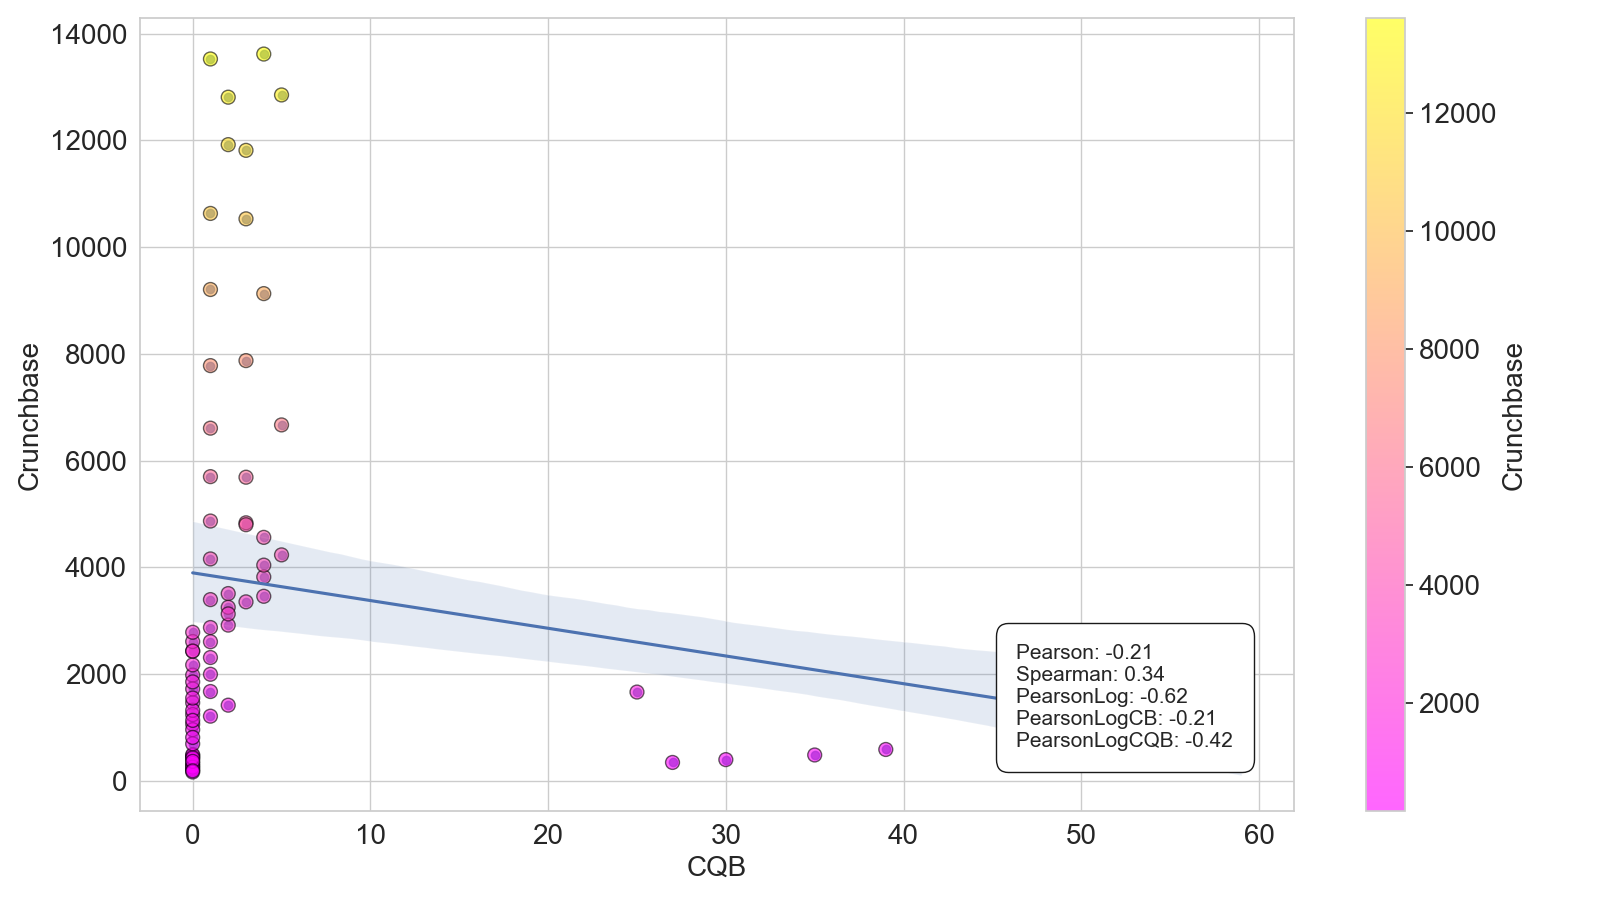
\includegraphics[width=1.0\textwidth]{images/crunchbase_academic_access/myplot.png}
    \caption{Confronto delle scorte ottenute dal Custom Query Builder e dall'Academic Reasearch Access per i paesi selezionati.}
    \label{fig:scrapervsapi}
\end{figure}


\section{Descrizione del dataset collezionato}
\label{sec:datasetcollezzionato}
L'intero dataset generato attraverso l'Academic Research Access contiene 1.288.646 profili utente.
Viene effettuata un'analisi per determinare gli stati per cui Crunchbase è più rappresentato. La prima fase di analisi viene effettuata attraverso una mappa di calore dell'utenza di Crunchbase per visualizzare quali sono le zone geografiche per cui la piattaforma è più utilizzata (Figure \ref{fig:crunchuserbaseheatmap}). La seconda fase prevede la creazione di un grafico che indica l'utenza nel tempo per i primi dieci stati per numero di utenti (Figura \ref{fig:lineplotutenza}). Entrambi i grafici sono stati realizzati usando i dati relativi a tutta l'utenza Crunchbase altamente qualificata per periodo compreso tra il 2010 ed il 2020. 
\begin{figure}[tb]
    \centering
    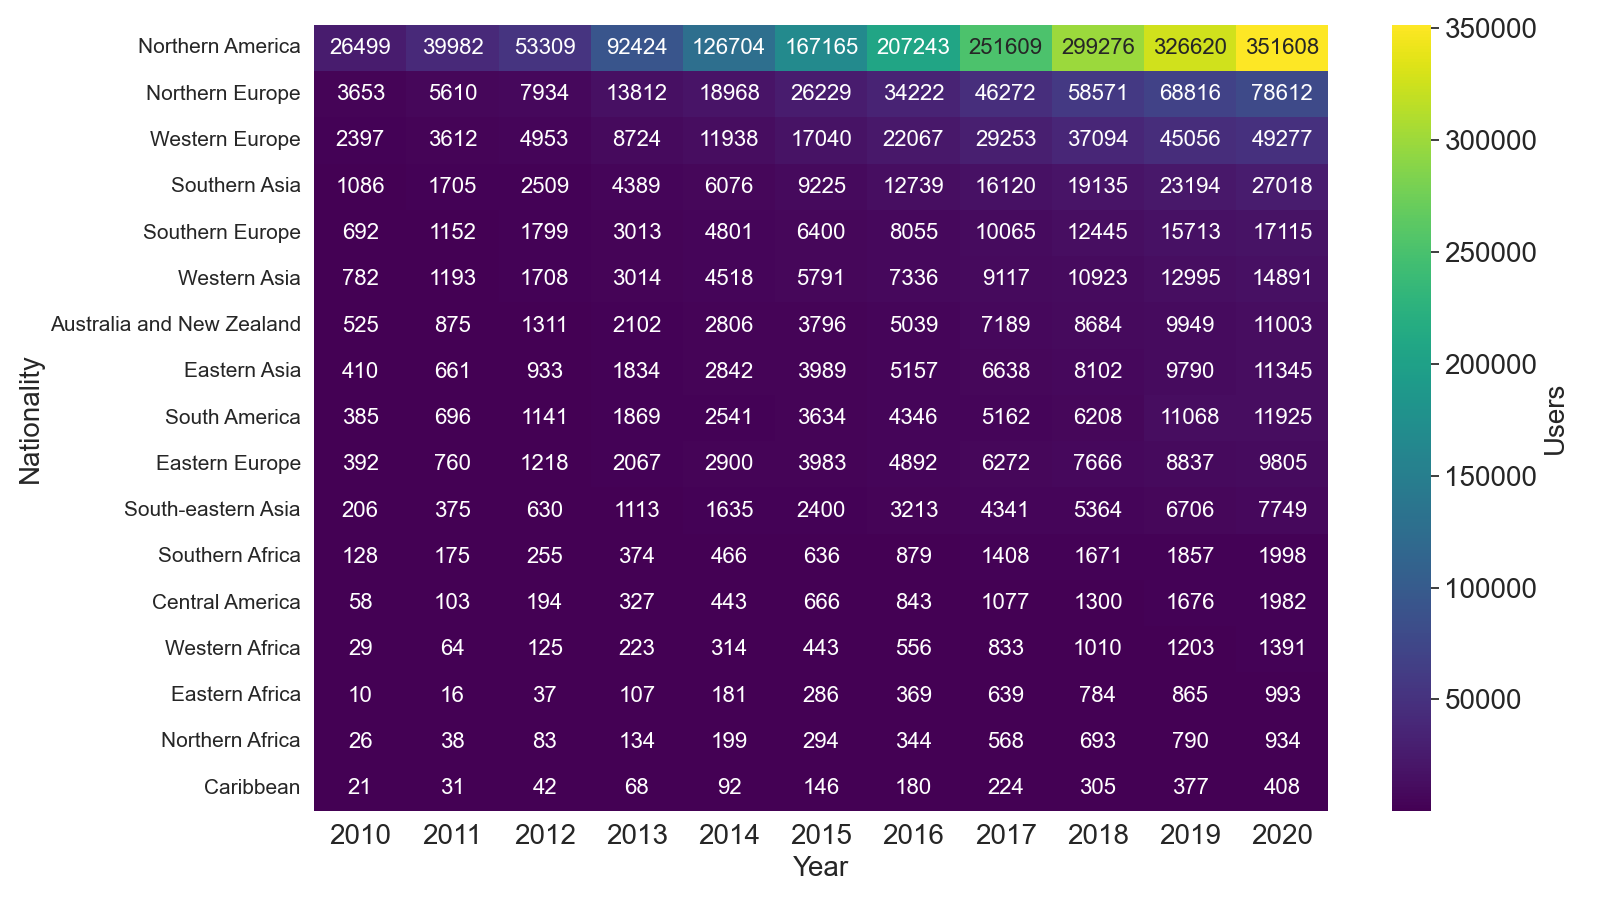
\includegraphics[width=\textwidth]{images/crunchbase_userbase/heatmap2.png}
    \caption{Utenza annuale di Crunchbase nel periodo 2010-2020 aggregata per zone geografiche}
    \label{fig:crunchuserbaseheatmap}
\end{figure}

La Figura \ref{fig:crunchuserbaseheatmap} mostra l'utenza annuale di Crunchbase (dal 2010 al 2020) in base alla nazionalità (inferita seguendo la definizione in Sezione \ref{preprocessing}). Si noti che le nazionalità sono state aggregate per sub continenti.
La crescita dell'utenza si osserva per tutti i paesi, in tutti i dieci anni osservati. Tuttavia, si nota che l'incremento nel numero di utenti è fortemente dipendente  dalle zone geografiche. L'America del nord è la zona con più utenti, seguita, seppur con larga differenza, dal nord e ovest Europa, e dal sud e ovest Asia. 

La Figura \ref{fig:lineplotutenza} mostra l'utenza Crunchbase dei dieci stati con più utenti sulla base della nazionalità. 
Per tutti e dieci i paesi si osserva una linea di valori monotona crescente, che indica che nel tempo la piattaforma è sempre più usata. 
\begin{figure}[tb]
\hfill
    \centering
    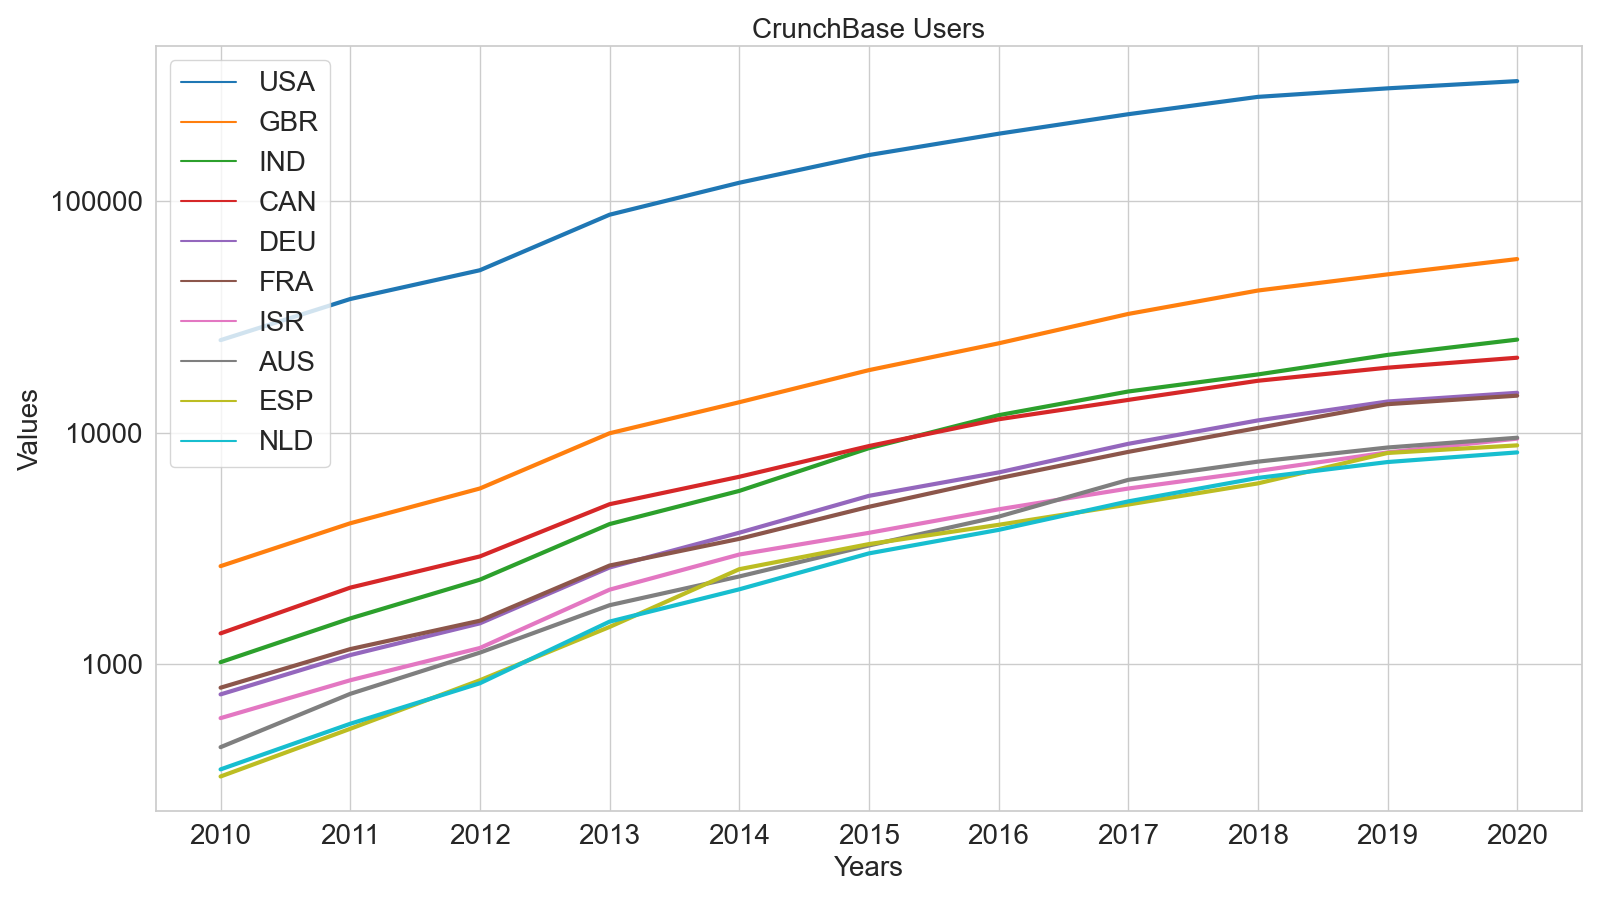
\includegraphics[width=1.0\textwidth]{images/crunchbase_userbase/lineplotlog.png}
    \caption{Trend utenza annuale di Crunchbase dal 2010 al 2020 per primi dieci paesi per numero di utenti totali al 2020.}
    \label{fig:lineplotutenza}
\end{figure}


I dati relativi a scorte e flussi estratti durante la fase di preprocessing (Sezione \ref{preprocessing}) sono stati analizzati per comprenderne la cardinalità. Il numero di scorte collezionate attraverso l'accesso accademico a Crunchbase è di 26.432. Ogni scorta è rappresentata da una tripla \texttt{nazionalità-statoScorte-anno}. 


I flussi, invece, hanno una cardinalità di 6716 combinazioni rappresentate da una tripla \texttt{origine-destinazione-anno}. Inoltre, ogni combinazione ha un valore per i residenti ed uno per i cittadini. 

\section{Analisi delle scorte}
\label{sec:analisi_scorte}
In questa sezione vengono analizzate le scorte di migranti di Crunchbase. 
Durante la fase iniziale, abbiamo analizzato le scorte lungo tutto l'arco temporale coperto dai dati (dal 2010 al 2020). 
Le scorte di Crunchbase sono state confrontate, mediante il calcolo della correlazione di Pearson e di Spearman, con le scorte in UN per gli anni 2010, 2015 e 2020. 
Per la visualizzazione dei risultati sono stati realizzati grafici di dispersione.

Per approfondire l'analisi, sono stati realizzati tre casi di studio. I primi due studi riguardano gli emigrati e immigrati italiani e britannici rispettivamente. Infine, il terzo caso analizzato si concentra sugli stati europei e nord americani. 

\subsection{Dati di Crunchbase}
\label{stockCrunchbase}
\begin{figure}[t]
    \centering
    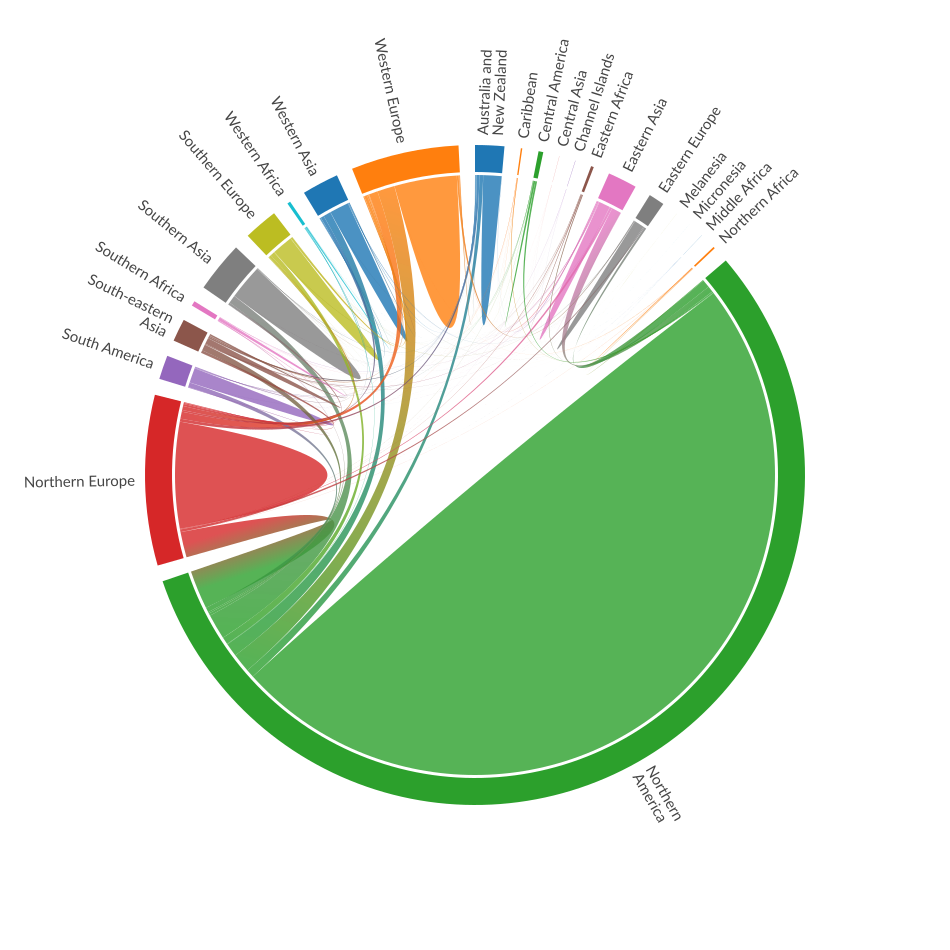
\includegraphics[width=\textwidth]{images/SVG/Chords/stocks/stock_chord_all.png}
    \caption{Scorte di migranti ottenute da Crunchbase sommate per il periodo 2010-2020.}
    \label{fig:chordCrunchbase_stock_all}
\end{figure}

Le scorte migratorie in Figura \ref{fig:chordCrunchbase_stock_all} sono in accordo con l'analisi dell'utenza Crunchbase effettuata in Sezione \ref{sec:datasetcollezzionato}. Ogni sezione del perimetro rappresenta una zona geografica, ogni arco rappresenta un numero di scorte di quella nazionalità rilevate nell'altro paese. Gli archi hanno dimensione differente in base alla dimensione delle scorte rilevate. La maggior parte degli utenti è rappresentato da nativi nord-americani residenti in nord America (non migranti). Osservando le singole zone, gli emigrati nord americani risiedono nell'ovest e nel nord Europa, e nel sud e est Asia. Inoltre, il nord America sembra accogliere il maggior numero di immigrati provenienti da tutte le zone, seppur in diversa misura.
Gli utenti del nord Europa e Europa dell'ovest sono rispettivamente il secondo e terzo gruppo più rappresentato. In entrambi i casi, così come per le altre zone, la maggior parte degli utenti è rappresentata da nativi. Nonostante ciò, parte degli utenti del nord Europa sembra essere emigrata in ovest Europa, e viceversa. 

\begin{figure}[htbp]
    \centering
    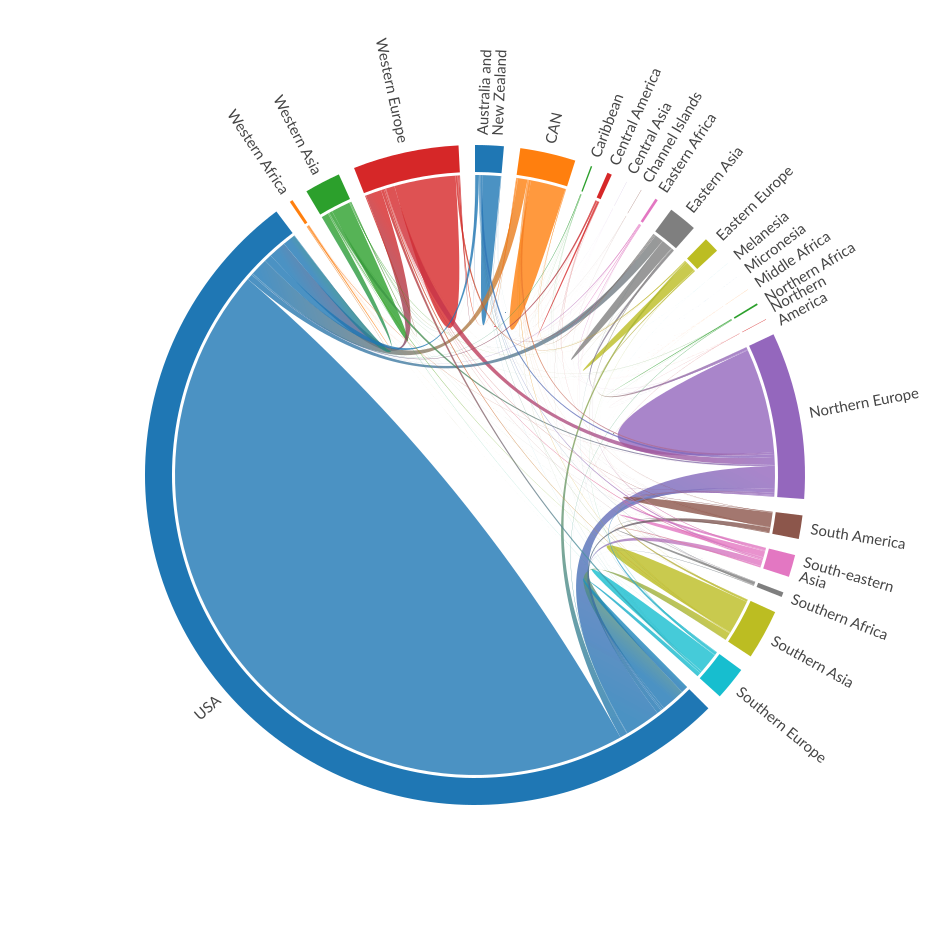
\includegraphics[width=0.9\textwidth]{images/SVG/Chords/stocks/stock_chord_USA_CAN_separate.png}
    \caption{Scorte migratorie aggregate per zone più Stati Uniti d'America e Canada. Le scorte sono sommate per il periodo dal 2010 al 2020.}
    \label{fig:chordCrunchbase_stock_usa_can}
\end{figure}

\begin{figure}[htbp]
    \centering
    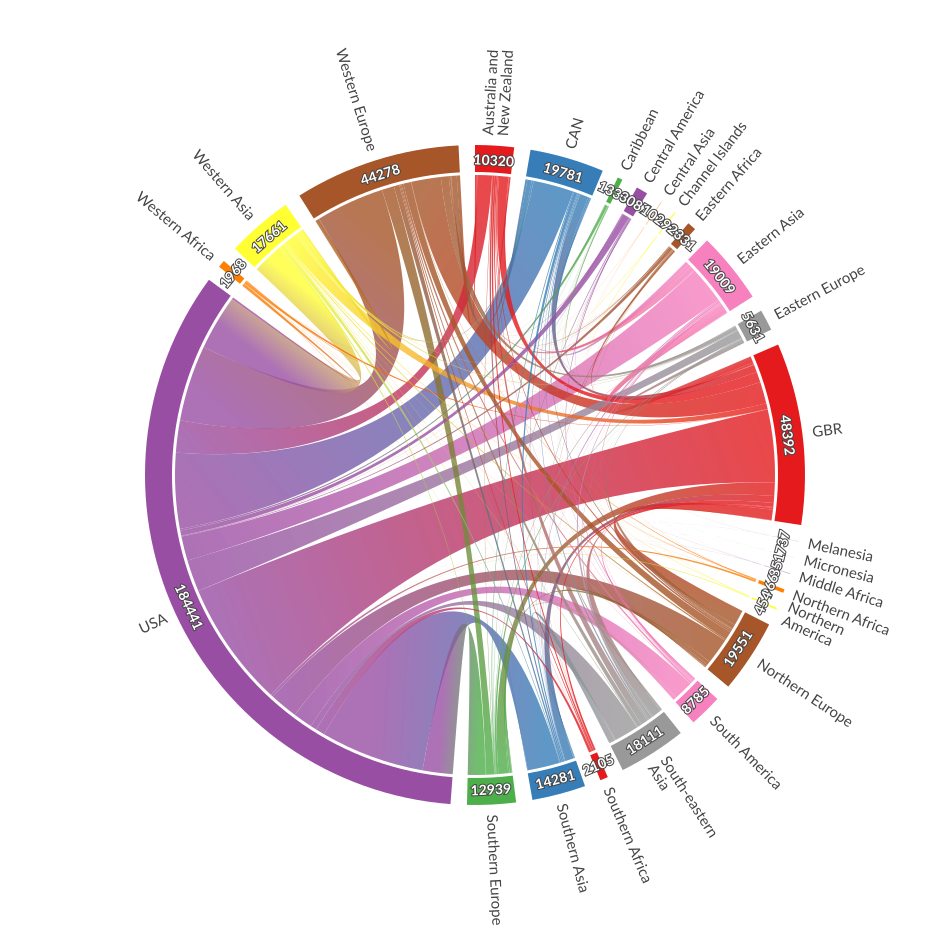
\includegraphics[width=0.9\textwidth]{images/SVG/Chords/stocks/stock_chord_USA_CAN_GBR_separate.png}
    \caption{Crunchbase scorte con Stati Uniti, Canada and Gran Bretagna separati dall'aggregazione.}
    \label{fig:chordCrunchbase_stock_usa_can_gbr}
\end{figure}

La Figura \ref{fig:chordCrunchbase_stock_usa_can} rappresenta le scorte migratorie, sommate dal 2010 al 2020, considerando Stati Uniti d'America e Canada come zone a sé stanti. Ogni sezione del perimetro del grafico rappresenta uno degli stati (USA o CAN) o la zona geografica.
Sebbene il grafico sia molto simile a quello in Figura \ref{fig:chordCrunchbase_stock_all}, sottolinea la differenza nel numero di immigrati/emigrati tra Stati Uniti d'America e Canada e tutte le altre zone. 


La Figura \ref{fig:chordCrunchbase_stock_usa_can_gbr} rappresenta tutte le scorte migratorie internazionali considerando Stati Uniti d'America, Canada e Gran Bretagna come zone a sé stanti, sommate dal 2010 al 2020. Gli archi hanno dimensione differente in base alla dimensione delle scorte rilevate su Crunchbase.  A differenza delle Figure \ref{fig:chordCrunchbase_stock_usa_can} e \ref{fig:chordCrunchbase_stock_all} i dati relativi a persone non migranti (e.g. Stati Uniti a Stati Uniti) non vengono considerati in questo grafico. Dalla figura si può notare la forte presenza di statunitensi in tutte le altre zone. Lo scambio di migranti più evidente è presente tra Stati Uniti e Gran Bretagna, a seguire ci sono in ordine il sud Asia, l'ovest dell'Europa e il Canada. L'Asia in tutte le sue coordinate presenta valori valori di scorte comparabili a quelli del nord Europa e del Canada.
\FloatBarrier
\subsection{Confronto Crunchbase con UN}

\label{UN_stock}
\begin{figure}[!h]
    \centering
    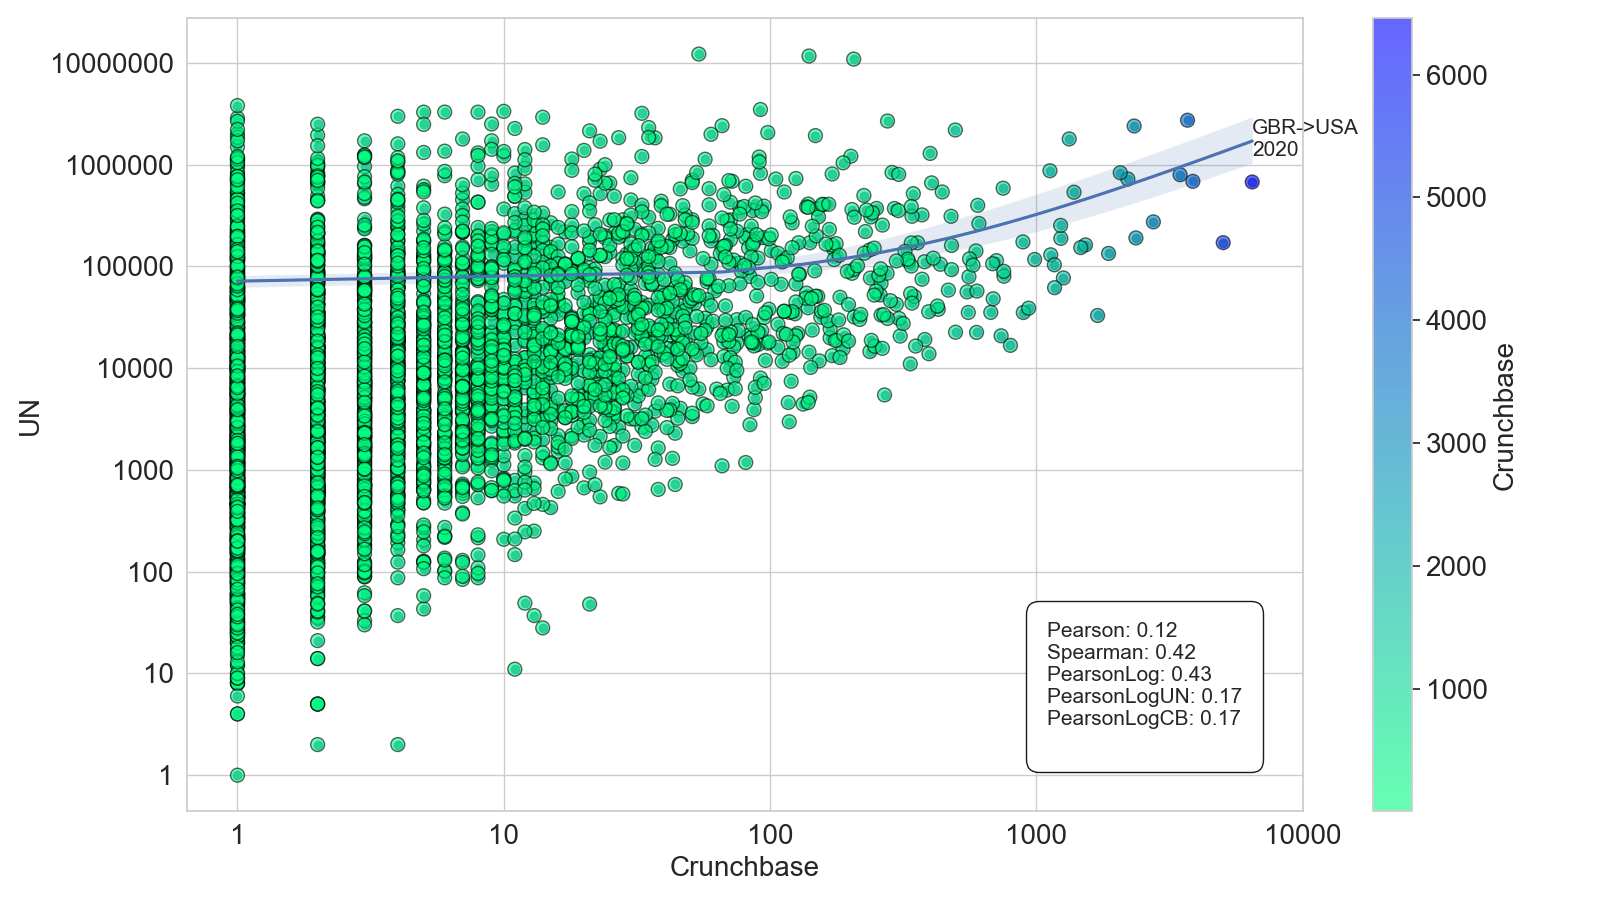
\includegraphics[width=0.8\textwidth]{images/Migration_Stocks/Migration Stocks.png}
    \caption{Confronto tra scorte di migranti in Crunchbase e UN. I dati sono per gli anni 2010, 2015 e 2020.}
    \label{fig:LogaritmicMigrationStocksScatterPlot}
\end{figure}
Il confronto delle scorte di Crunchbase con quelle di UN comporta la selezione delle combinazioni comuni di paesi. Inoltre, come descritto in precedenza (Sezione \ref{DatiTradizionali}), UN dispone di dati solo di dati quinquennali, nel nostro caso abbiamo selezionato gli anni 2010, 2015 e 2020. Questo duplice processo di selezione (coppie comuni e anni) riduce le combinazioni a 5295 (-21137).
Il grafico in Figura  \ref{fig:LogaritmicMigrationStocksScatterPlot} mostra la correlazione tra le scorte di Crunchbase e di UN, utilizzando una scala logaritmica per entrambi gli assi. Sull'asse x si hanno i dati Crunchbase, sull'asse y i dati UN. Il valore massimo ottenuto per le scorte Crunchbase è rappresentato accanto al punto relativo al suo valore, con la forma \textit{Nazionalità->Paese delle scorte Anno}. Nel riguardo in basso a destra sono presenti le varie correlazioni calcolate. La correlazione di Pearson è di 0.12, mentre l'indice di Spearman è di 0.42. Il coefficiente di Spearman ci indica che sia presente una correlazione debole tra le scorte in Crunchbase ed UN. Se si trasformano i dati delle scorte (UN e Crunchbase) in scala logaritmica per il calcolo della correlazione di Pearson, il valore è di 0.43 confermando il risultato ottenuto con il coefficiente di Spearman.
\FloatBarrier
\subsection{Caso di studio: Italia}
\label{itastock}
\begin{figure}[tbp]
  \centering
  \begin{minipage}[t]{0.8\textwidth}
    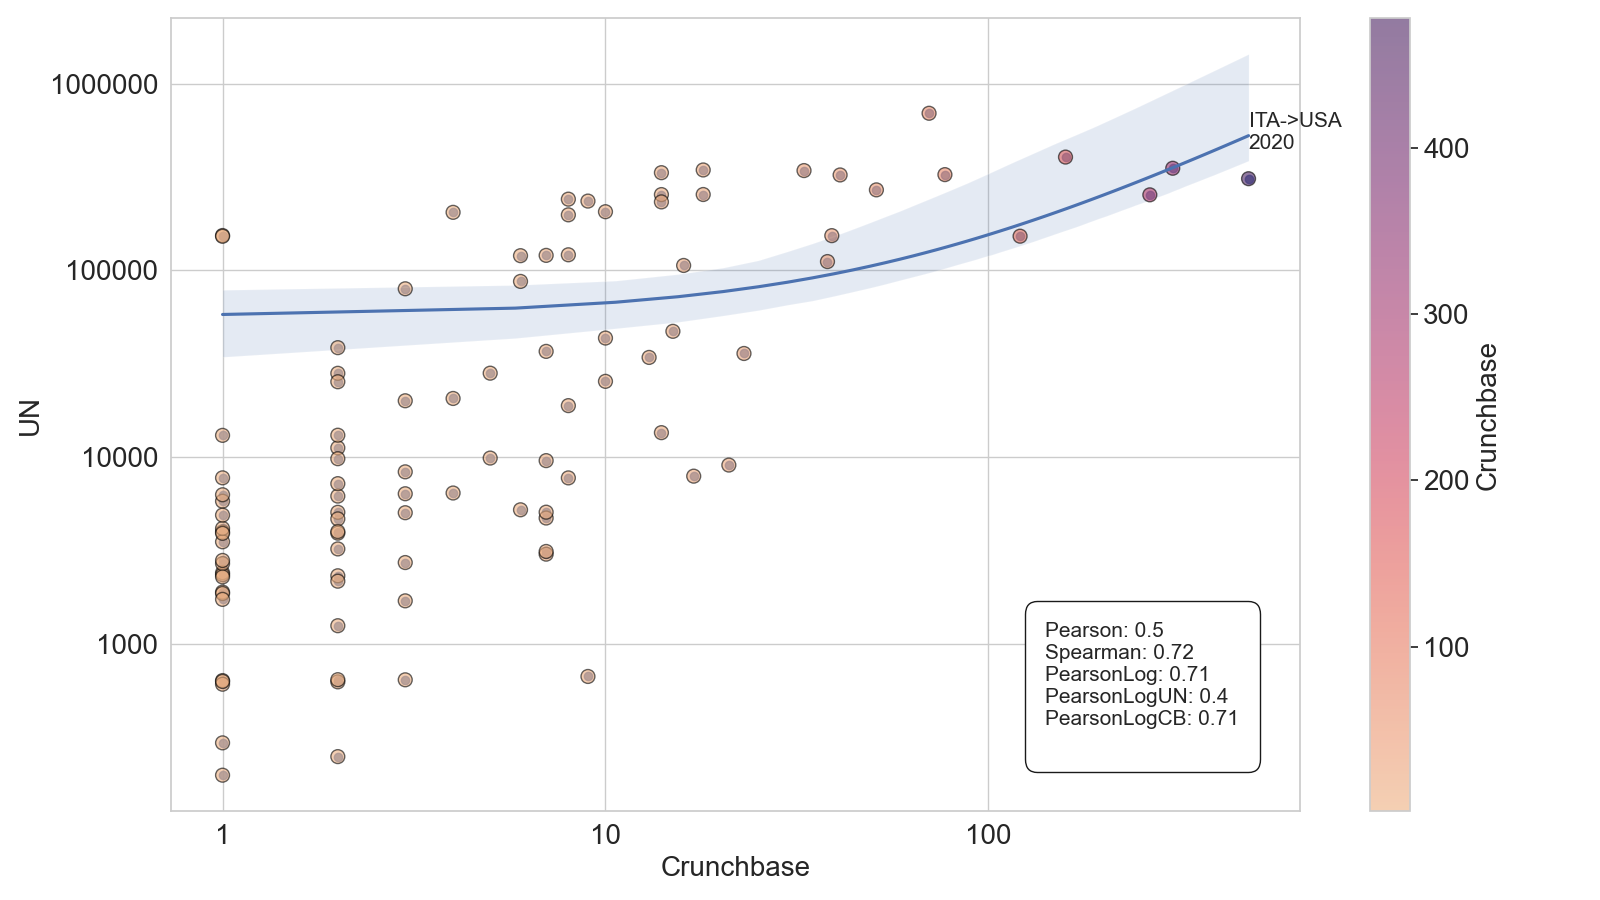
\includegraphics[width=\textwidth]{images/Migration_Stocks/ITA/Migration Stocks from ITA.png}
    \caption{Emigrati italiani nel mondo, confronto per gli anni 2010, 2015 e 2020 tra Crunchbase e UN.}
    \label{fig:MigrationstockswithItalianNationality}
  \end{minipage}
  %\hfill
  \begin{minipage}[b]{0.8\textwidth}
    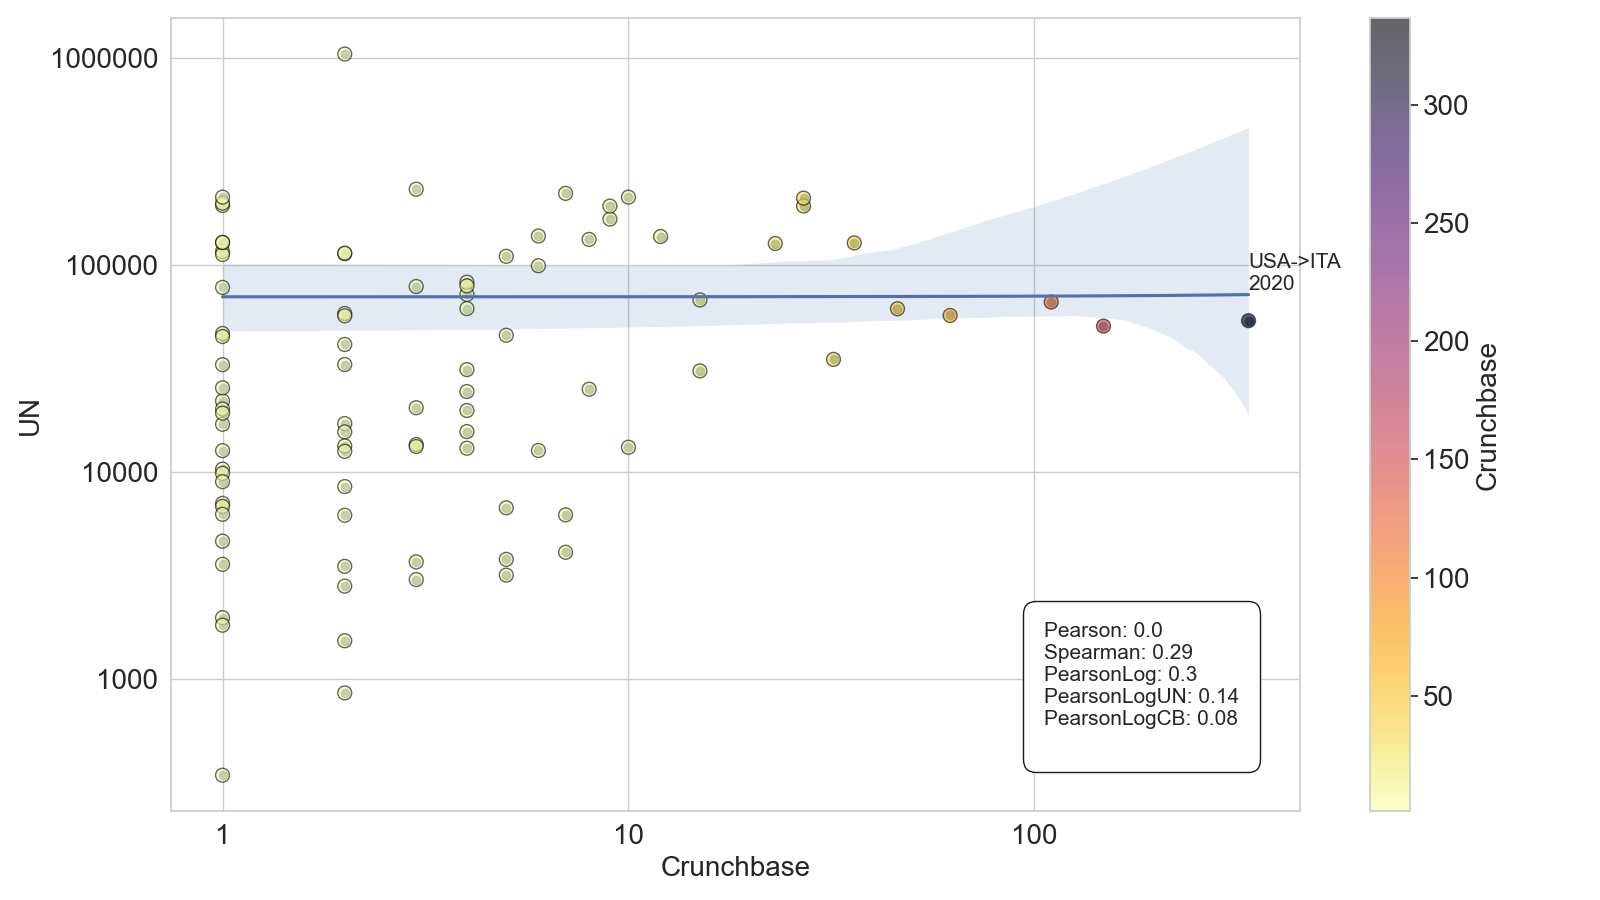
\includegraphics[width=\textwidth]{images/Migration_Stocks/ITA/Migration Stocks to ITA.png}
    \caption{Immigrati in Italia, confronto per gli anni 2010, 2015 e 2020 tra Crunchbase e UN. }
    \label{fig:MigrationstocktoItaly}
  \end{minipage}
\end{figure}

In questo studio vengono analizzate le scorte di migranti di nazionalità italiana nel mondo e le scorte di migranti in Italia. Lo studio è svolto per gli anni 2010, 2015 e 2020. 
La Figura \ref{fig:MigrationstockswithItalianNationality} mostra il confronto delle scorte di emigranti di nazionalità italiana tra UN e Crunchbase per gli anni 2010, 2015 e 2020. A destra la barra che indica i valori relativi ai vari colori, e il riquadro contenente le correlazioni calcolate. In basso il riquadro contenente le varie correlazioni calcolate. Come per il confronto precedente (Sezione \ref{UN_stock}), il valore massimo ottenuto per le scorte Crunchbase è rappresentato accanto al punto relativo al suo valore, con la forma \textit{Nazionalità->Paese delle scorte Anno}. La maggior parte delle scorte di italiani altamente qualificati per Crunchbase risiede negli Stati Uniti.
La correlazione di Pearson è 0,5 e l'indice di Spearman 0.72. La correlazione di Pearson, si eguaglia all'indice di Spearman (0.71) se le scorte in ingresso (UN e Crunchbase) sono poste in scala logaritmica. Questo ci indica una forte correlazione tra i dati UN e Crunchbase per le scorte di italiani fuori sede. 
Inoltre, il grafico in Figura \ref{fig:MigrationstocktoItaly} mostra il confronto tra le scorte di immigrati in Italia da Crunchbase e UN. La correlazione di Pearson in questo confronto ha valore zero, cioè indica che non c'è correlazione.
La correlazione di Pearson vede un incremento positivo fino a 0.3, se poniamo le scorte delle fonti (UN e Crunchbase) in scala logaritmica. L'indice di Spearman invece ha un valore di 0.29. Sebbene i valori dei coefficienti incrementino, non è sufficiente per determinare una correlazione debole.


\FloatBarrier
\subsection{Caso di studio: Gran Bretagna}
\label{gbrstock}
\begin{figure}[tbp]
  \centering
  \begin{minipage}[t]{1\textwidth}
    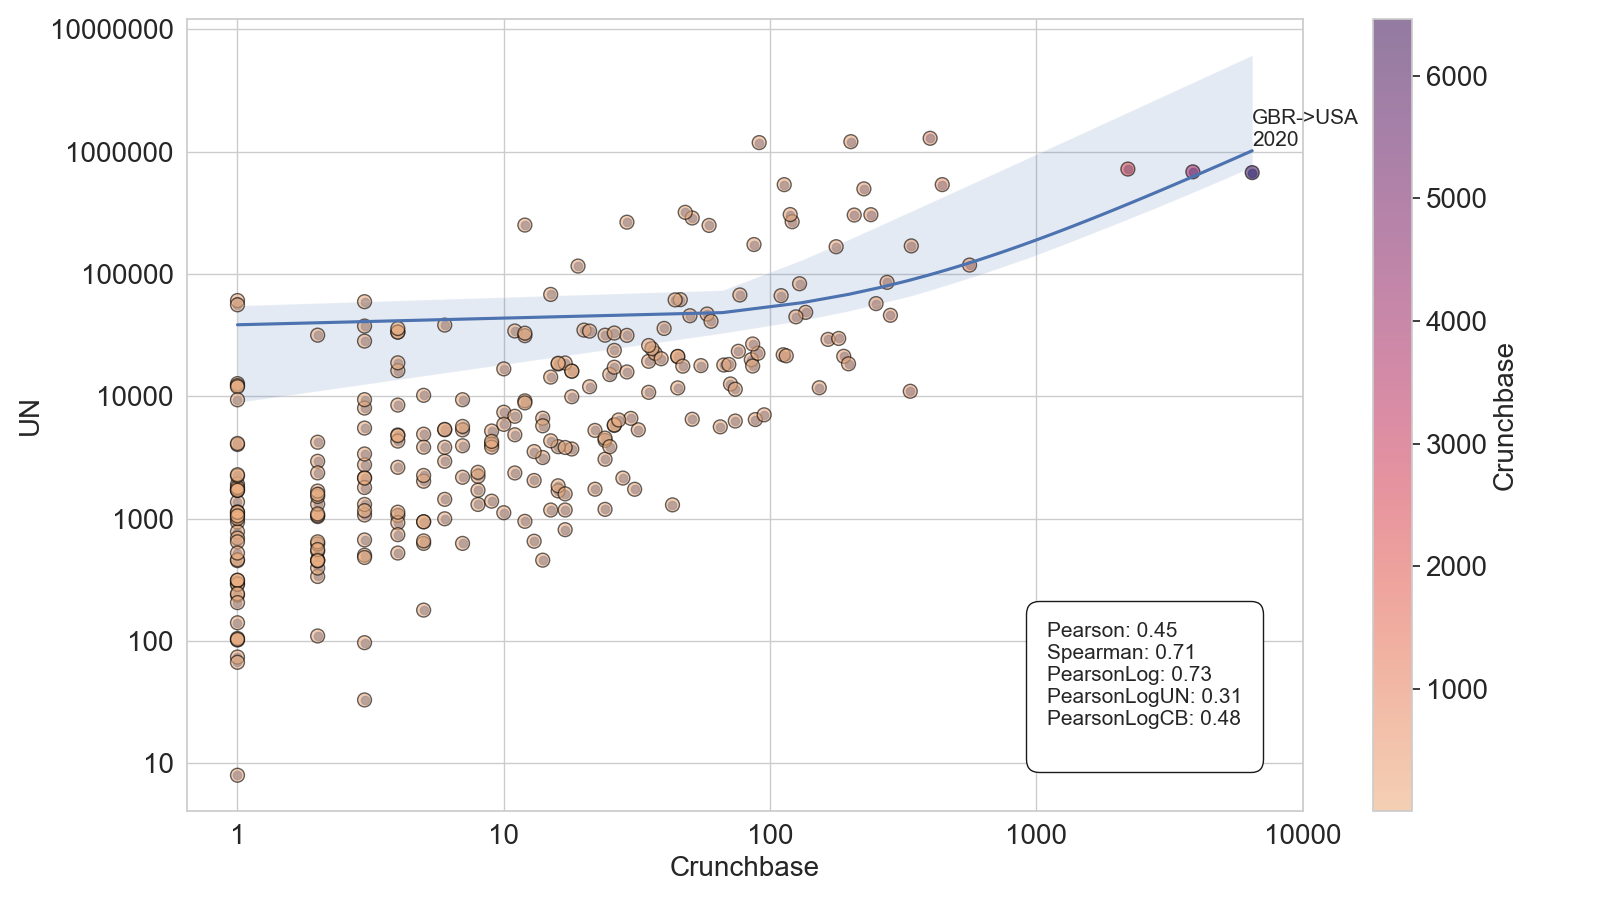
\includegraphics[width=\textwidth]{images/Migration_Stocks/GBR/Migration Stocks from GBR.png}
    \caption{Emigrati britannici nel mondo, confronto per gli anni 2010, 2015 e 2020 tra Crunchbase e UN.}
    \label{fig:Migrationstockfromgbr}
  \end{minipage}
  %\hfill
  \begin{minipage}[b]{1\textwidth}
    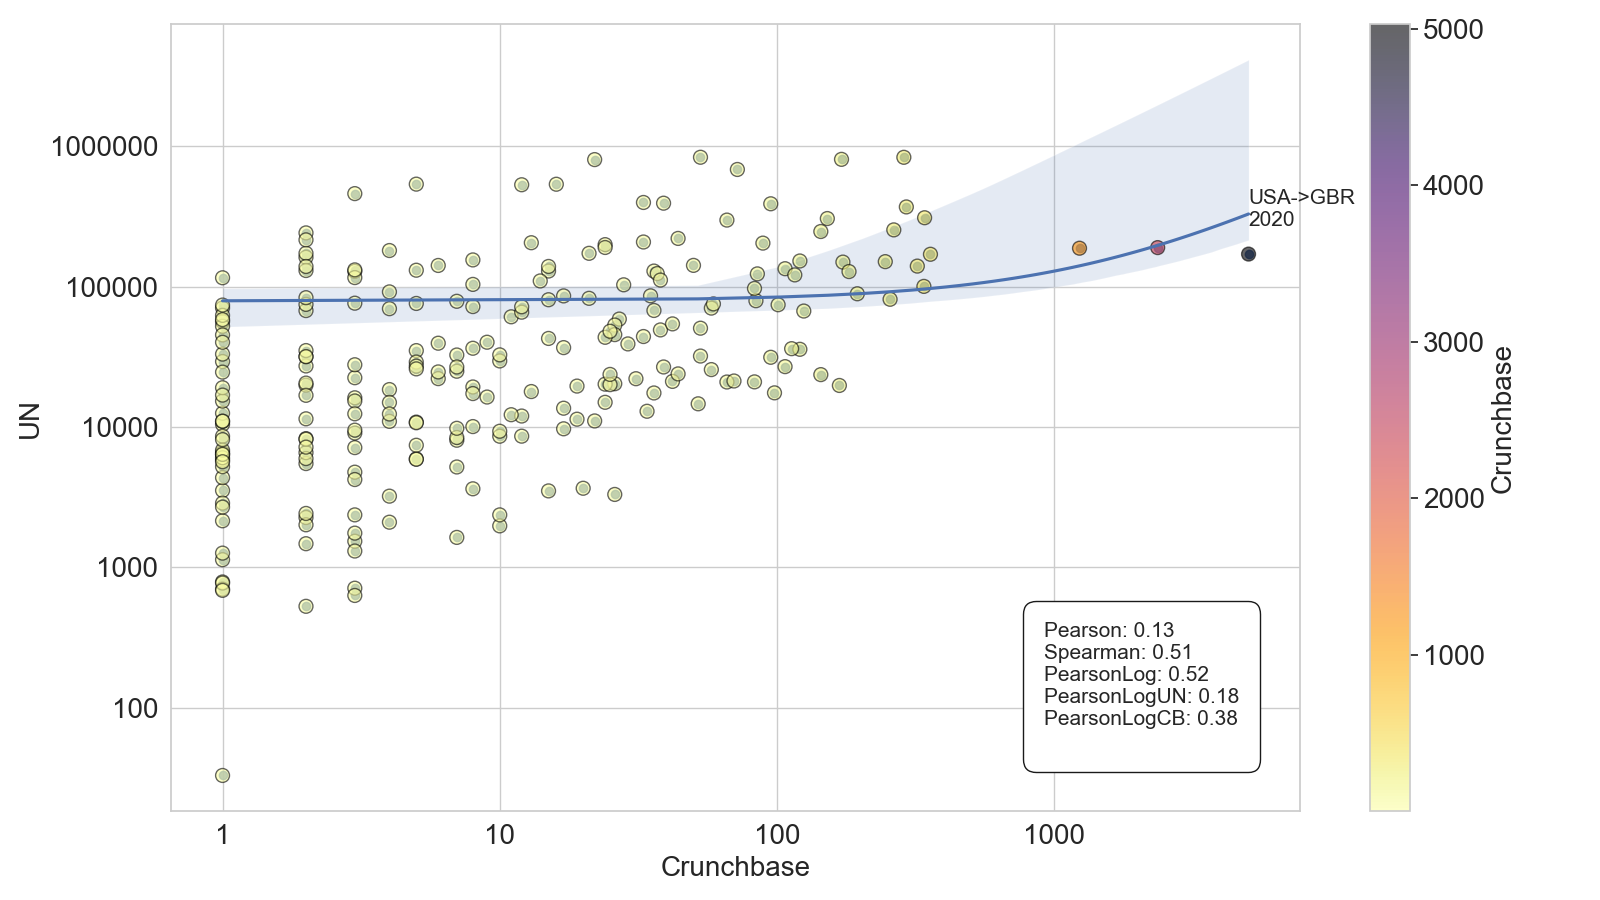
\includegraphics[width=\textwidth]{images/Migration_Stocks/GBR/Migration Stocks to GBR.png}
    \caption{Immigrati in Gran Bretagna, confronto per gli anni 2010, 2015 e 2020 tra Crunchbase e UN.}
    \label{fig:Migrationstocktogbr}
  \end{minipage}
\end{figure}

Le scorte relative a cittadini di nazionalità britannica emigrati, in Figura \ref{fig:Migrationstockfromgbr}, mostrano il valore massimo per gli Stati Uniti(circa 6.000). 
Entrambi gli indici di Pearson e Spearman mostrano correlazioni positive, di 0.45 e 0.71, rispettivamente.
La correlazione di Pearson calcolata con entrambe le variabili in scala logaritmica restituisce valori intorno a 0.73, denotando un buon livello di correlazione.

Per quanto riguarda le scorte migratorie della Gran Bretagna, il grafico in Figura \ref{fig:Migrationstocktogbr} mostra una correlazione di Pearson di 0.13 e dei valori più alti rispetto a quelli osservati per l'Italia (Figura \ref{fig:MigrationstocktoItaly}). L'indice di Spearman ha un valore di 0.51, quasi identico a quello di Pearson (0.52) quando le scorte sono poste in scala logaritmica. Le scorte più numerose in Gran Bretagna nel 2020 erano di nazionalità statunitense. Il valore massimo delle scorte di migranti in Gran Bretagna (5000) è tra i più altri osservati.

\FloatBarrier
\subsection{Caso di studio: Europa e nord America}
\label{europenordamstock}
\begin{figure}[tbp]
  \centering
  \begin{minipage}[t]{1\textwidth}
    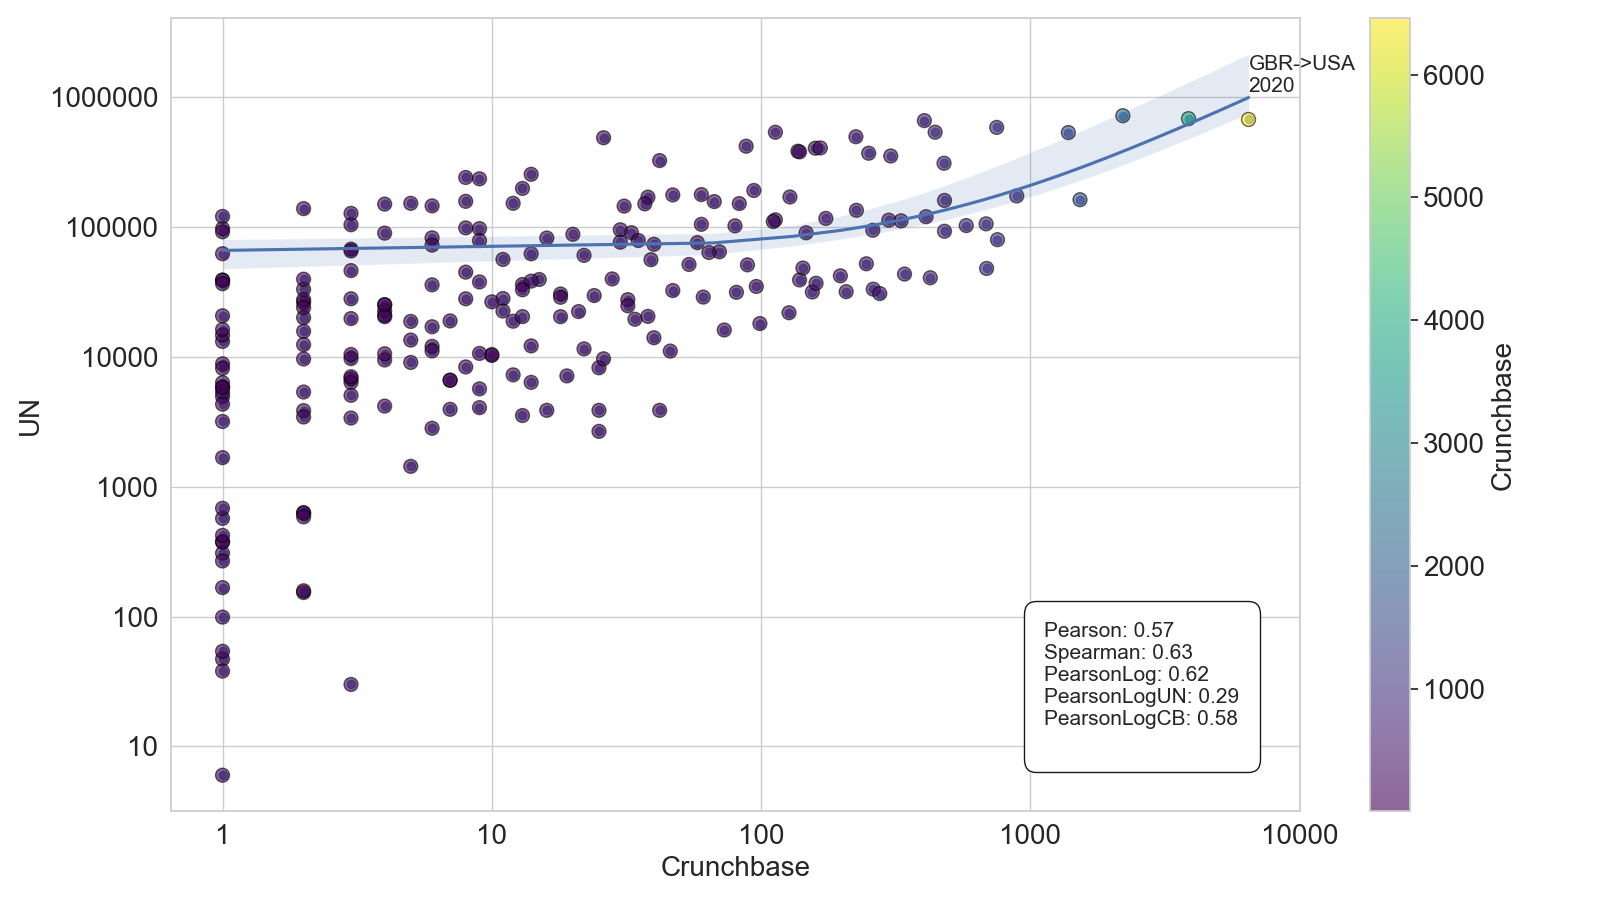
\includegraphics[width=\textwidth]{images/Migration_Stocks/NORTHAMERICA_EUROPE/Migration Stocks from Europe to North America.png}
    \caption{Scorte di migranti di nazionalità Europea in nord America (2010, 2015 e 2020).}
    \label{fig:migstockresNordAmnatEur}
  \end{minipage}
  %\hfill
  \begin{minipage}[b]{1\textwidth}
    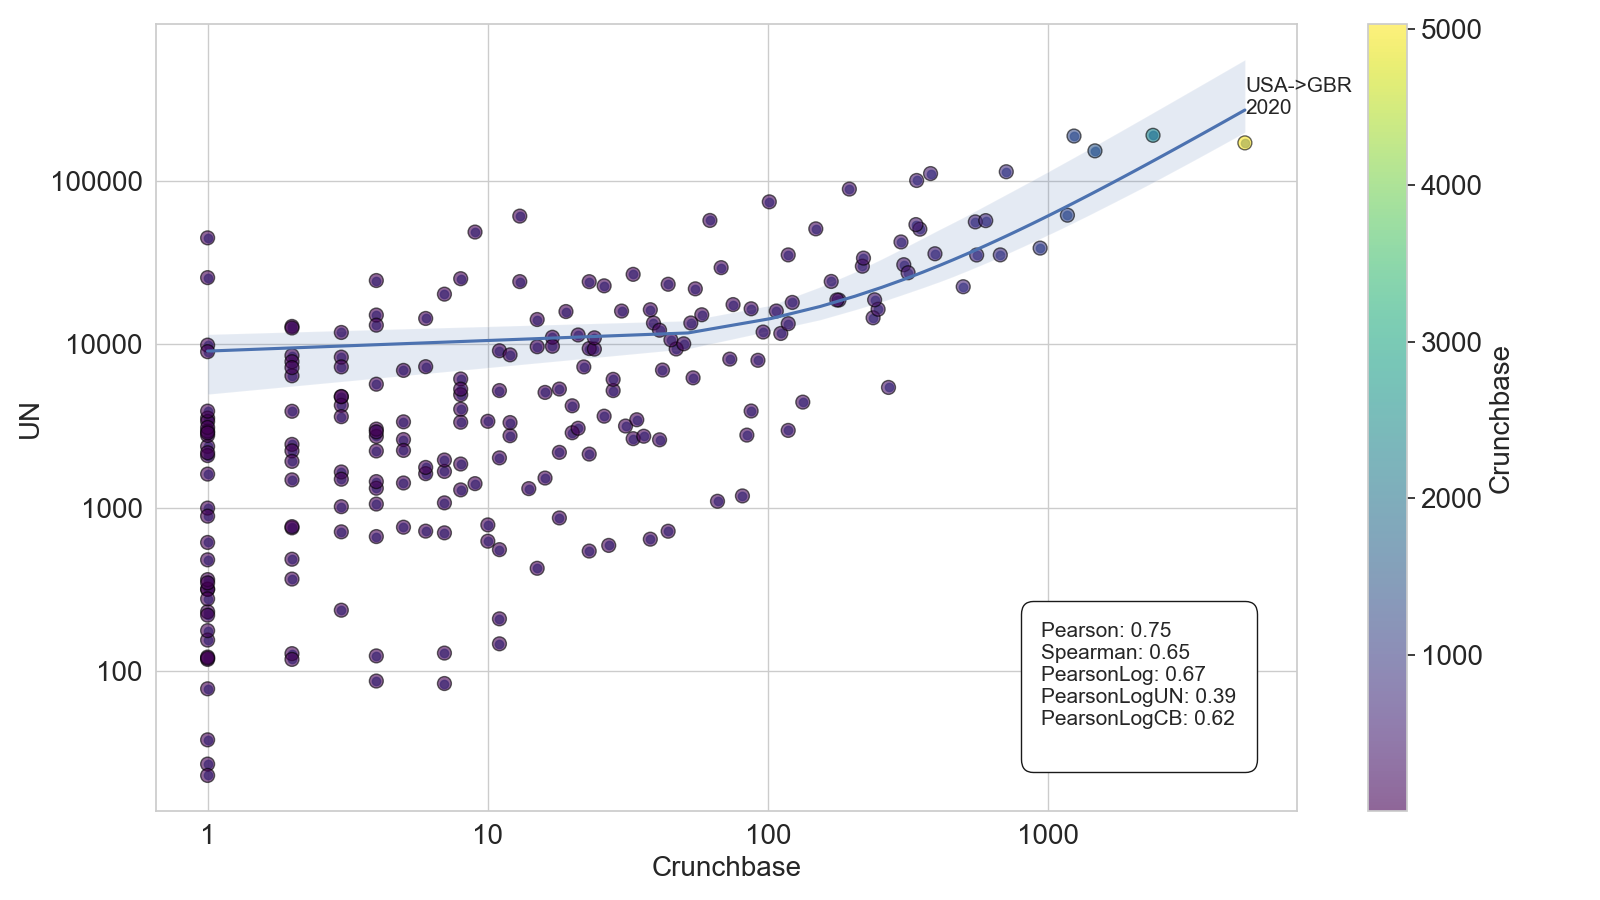
\includegraphics[width=\textwidth]{images/Migration_Stocks/NORTHAMERICA_EUROPE/Migration Stocks from North America to Europe.png}
    \caption{Scorte di migranti di nazionalità nord americana in Europa (2010, 2015 e 2020).}
    \label{fig:migstockresEuropenatNordAm}
  \end{minipage}
\end{figure}
Viene effettuato un filtro sui dati Crunchbase e UN per il continente Europa e il subcontinente nord americano. Il grafico in Figura \ref{fig:migstockresNordAmnatEur} analizza le scorte migratore di persone di nazionalità europea in nord America. Sull'asse delle x vengono posti i valori Crunchbase, sull'asse delle y i valori UN. In questo caso, la correlazione di Pearson è di 0.57 e l'indice di Spearman di 0.63. La correlazione di Pearson ponendo le scorte in scala logaritmica si eguaglia all'indice di Spearman (0.62).
Questi risultati suggeriscono quindi dei buoni livelli di correlazione. Il valore massimo di scorte di migranti altamente qualificati per Crunchbase, indicato nel grafico accanto al punto, è di britannici in nord America.
In Figura \ref{fig:migstockresEuropenatNordAm} viene mostrato il confronto delle scorte di nazionalità nord americana in Europa. 
La correlazione di Pearson è di 0.75 e l'indice di Spearman di 0,65, indicando una correlazione positiva forte per Pearson. Il valore di scorte maggiori per Crunchbase si ottiene per i migranti statunitensi in Inghilterra nel 2020.
Come già mostrato durante l'analisi dell'utenza di Crunchbase (Sezione \ref{sec:datasetcollezzionato}), Europa e Nord America sono le zone più rappresentate.
\FloatBarrier

\subsection{Discussione}
Dato che a differenza di Crunchbase, UN dispone di sole scorte quinquennali, sono stati analizzati dati relativi al 2010, 2015 e 2020
Le scorte migratorie di Crunchbase presentano una correlazione debole con UN nel caso generale (Sezione \ref{UN_stock}).
Il caso di studio dell'Italia (Sezione \ref{itastock}) mostra correlazioni discrete per gli emigrati dall'Italia, ma nessuna correlazione per gli immigrati in Italia.
Per il caso di studio della Gran Bretagna (Sezione \ref{gbrstock}) sia le scorte di emigrati che di immigrati hanno correlazione discreta con UN.
L'ultimo caso di studio si focalizza sugli stati del continente europeo e sul nord America (Sezione \ref{europenordamstock}). La correlazione è discreta per gli emigrati europei in nord America. Inoltre, Pearson indica una forte correlazione per gli immigrati nord americani in Europa. 
I risultati ottenuti suggeriscono che a seconda dei casi e soggetti di studio, i dati di Crunchbase potrebbero essere impiegati per lo studio delle scorte di migranti. 

\section{Analisi dei flussi}
\label{sec:analisi_flussi}
In questa sezione vengono analizzati flussi di migranti di Crunchbase aggregati per zona geografica.
Oltre allo studio dei flussi aggregati, per la Gran Bretagna è stato analizzato il periodo connesso alla Brexit (Sezione \ref{brexitflowscrunch}).
I flussi di Crunchbase sono stati confrontati, mediante il calcolo della correlazione di Pearson e di Spearman, con i flussi in UN, Eurostat e con l'unione dei due, per gli anni dal 2010 al 2020.
I risultati dello studio dei flussi aggregati per paesi lungo tutto l'arco temporale coperto dai dati (dal 2010 al 2020) sono stati visualizzati mediante chord diagram.
Per il caso studio relativo all'Italia è stato impiegato il solo dataset dei flussi Eurostat. Per la Gran Bretagna è stata usata l'unione dei flussi in UN ed Eurostat. 
Come per le scorte (Sezione \ref{stockCrunchbase}) la visualizzazione dei risultati avviene attraverso grafici di dispersione.
\FloatBarrier
\subsection{Dati di Crunchbase} 
\label{flowscrunch}

\begin{figure}[tbp]
    \begin{subfigure}{0.48\textwidth}
        %\raggedleft         
        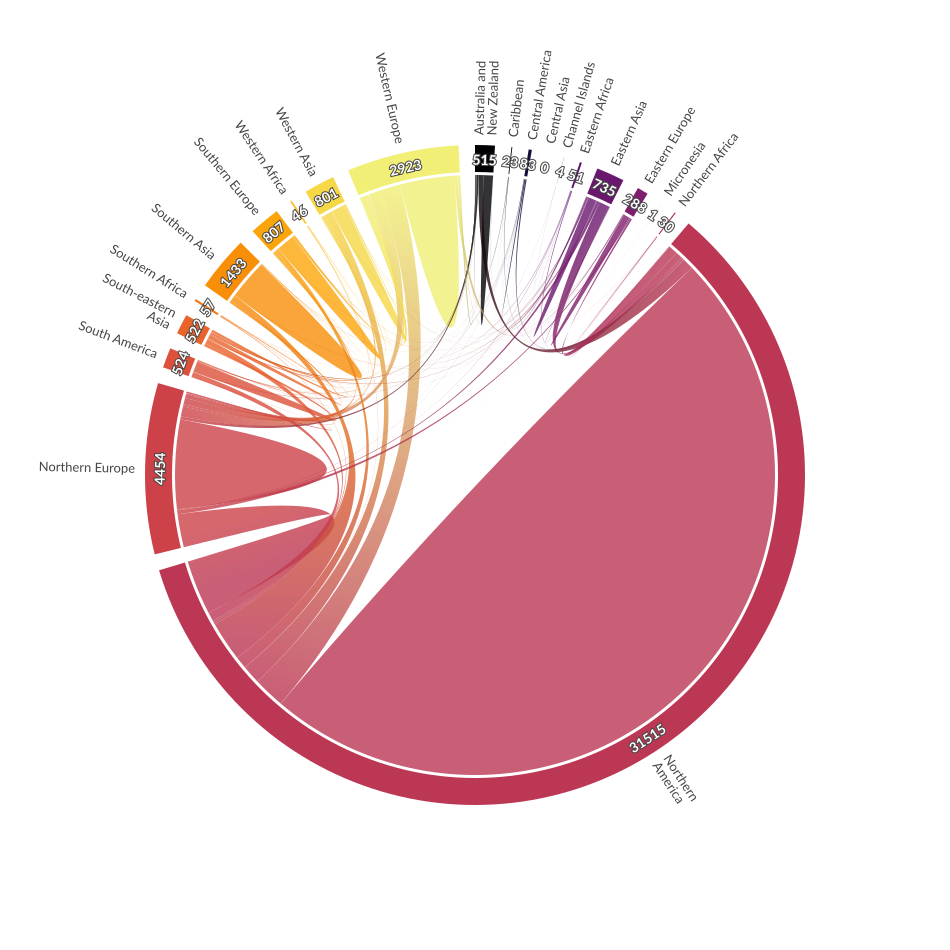
\includegraphics[scale=0.34]{images/SVG/Chords/Crunchbase/Crunchbase_Cit_Red.png}
        \caption{Flussi di cittadini}
        \label{fig:chordCrunchbase_cit}
    \end{subfigure}
    \begin{subfigure}{0.48\textwidth}
        %\raggedleft         
        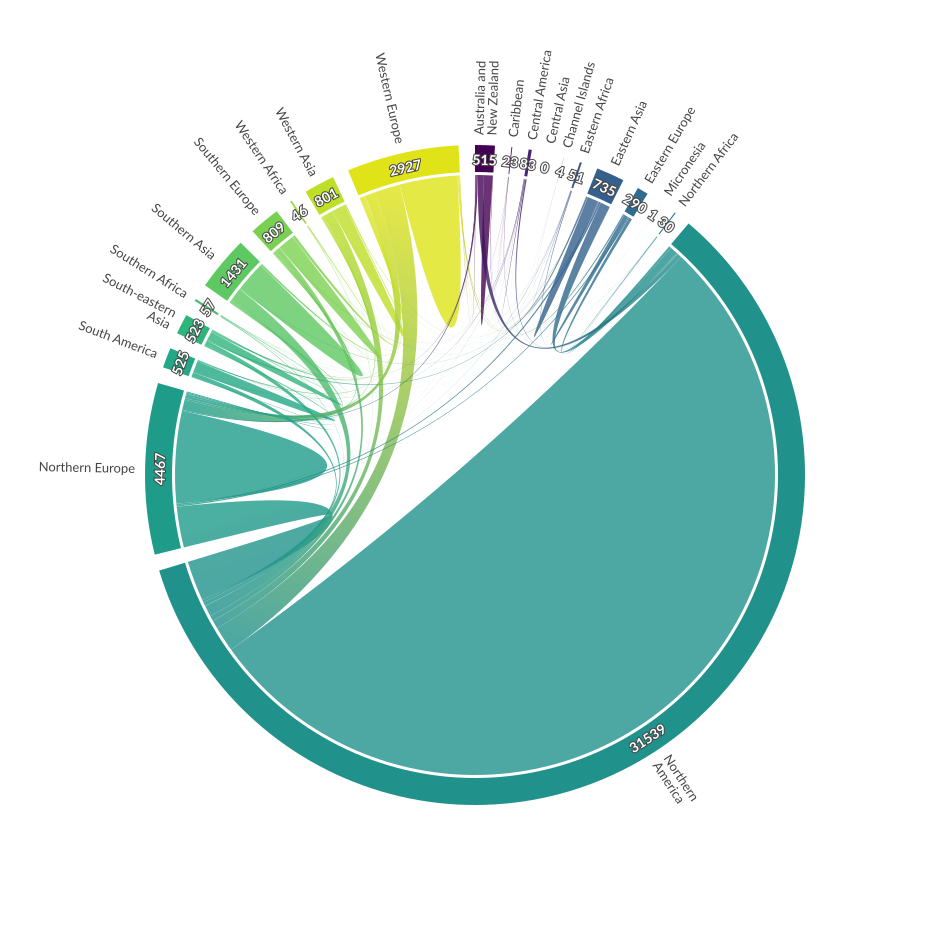
\includegraphics[scale=0.34]{images/SVG/Chords/Crunchbase/Crunchbase_Res_Blue.png}
        \caption{Flussi di residenti}
        \label{fig:chordCrunchbase_res}
    \end{subfigure}
    \caption{Flussi di migranti da Crunchbase aggregati per zone geografiche, dal 2010 al 2020. Il numero relativo alla zona indica il numero di flussi uscenti.}
    \label{fig:chordCrunchbase}
\end{figure}

I flussi in Figura \ref{fig:chordCrunchbase_cit} relativi a tutti i cittadini (utenti che sono residenti nello stato della nazionalità) presenti su Crunchbase sono maggiori per il nord America, il nord Europa e l'Europa dell'ovest. 
Buona parte dei flussi sono rappresentati da persone che si spostano in paesi della stessa zona, in particolare per il nord America. \par

La Figura \ref{fig:chordCrunchbase_res} rappresenta i flussi migratori dei residenti osservabili dai dati di Crunchbase. 
I flussi dei residenti sono simili a quelli dei cittadini (Sezione \ref{flowscrunch}). I flussi del nord America si presentano, anche in questo caso, i più numerosi. 

%Questo suggerisce che gli utenti su Crunchbase che migrano siano sia cittadini che residenti nello stato di provenienza. 
Inoltre, i risultati mostrano che la distribuzione dei flussi migratori su Crunchbase è maggiore per il subcontinente nord americano e per l'Europa. Tuttavia, sono presenti flussi relativi anche agli altri sub-continenti, sebbene siano minori. 
\FloatBarrier

\subsubsection{Caso di studio: Gran Bretagna e la Brexit}
\label{brexitflowscrunch}


\begin{figure}[!h]
    \centering
    \begin{subfigure}{0.47\textwidth}
        \raggedleft         
        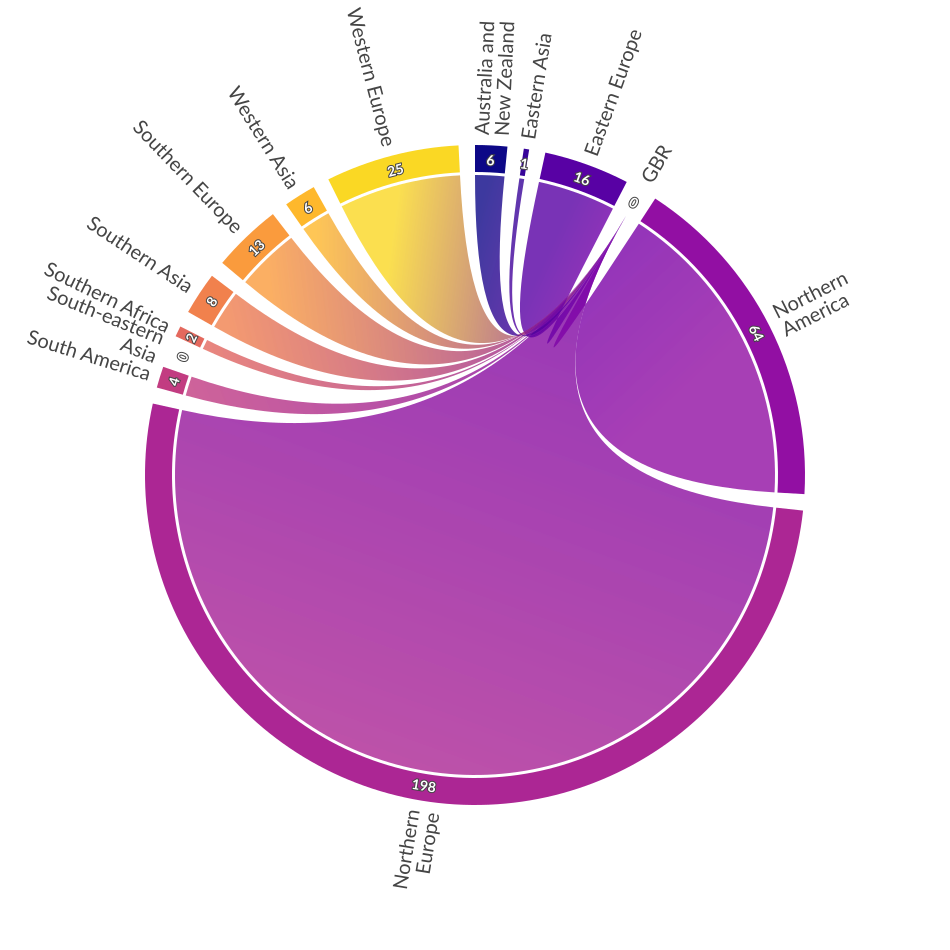
\includegraphics[scale=0.34]{images/SVG/Chords/Brexit/togbrflows_2015.png}
        \caption{Flussi 2015}
        \label{fig:togbr_flowsBrexit2015}
    \end{subfigure}
    \begin{subfigure}{0.47\textwidth}
        \raggedleft         
        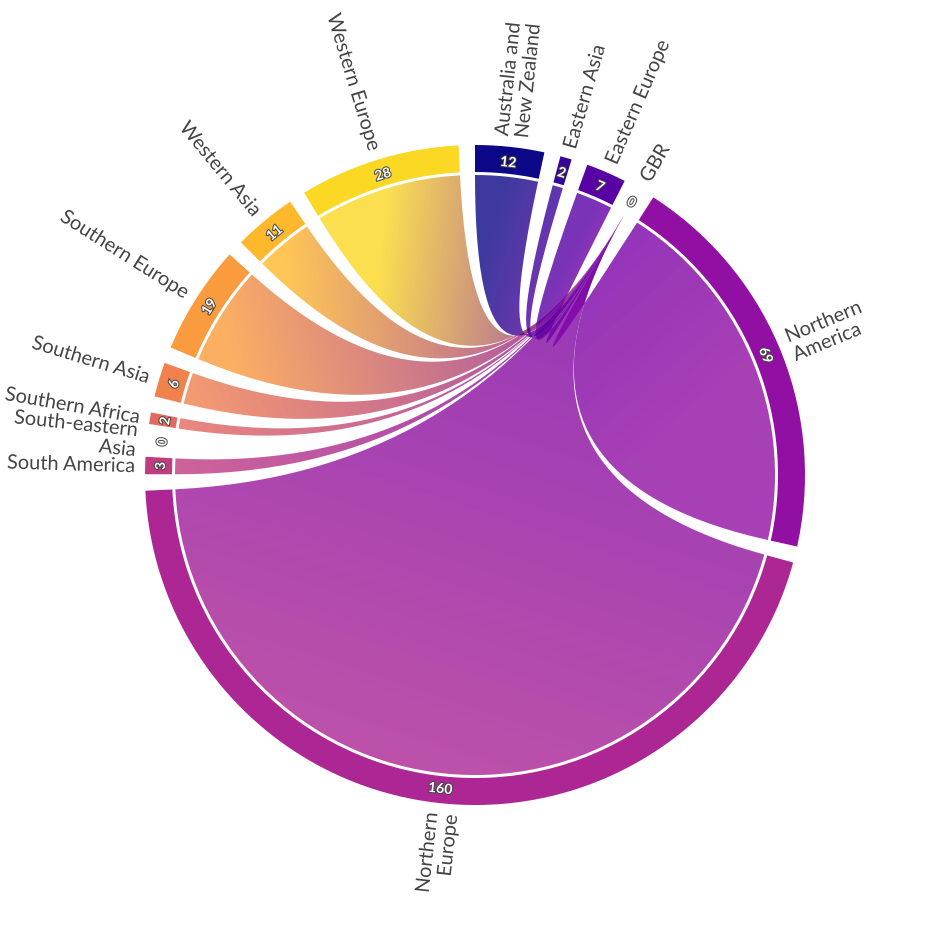
\includegraphics[scale=0.34]{images/SVG/Chords/Brexit/togbrflows_2017.png}
        \caption{Flussi 2017}
        \label{fig:togbr_flowsBrexit2017}
    \end{subfigure}
    \caption{Flussi di immigrati in Gran Bretagna da Crunchbase, per gli anni 2015 e 2017.}
    \label{fig:togbr_flowsBrexit}
\end{figure}


La Figura \ref{fig:togbr_flowsBrexit2015} mostra i flussi di immigrati, in Crunchbase, che interessano la Gran Bretagna nell'anno 2015. Gli stati vengono aggregati per zona, il numero relativo alla zona indica il numero di flussi uscenti. I flussi di emigrati dalla Gran Bretagna sono stati ignorati lasciando spazio ai flussi di immigrati nel grafico. I flussi maggiori provengono dal nord Europa, il nord America e l'Europa dell'ovest. 
La Figura \ref{fig:togbr_flowsBrexit2017} mostra i flussi di migranti, da Crunchbase, verso la Gran Bretagna nel 2017. La Figura mostra leggere differenze nei flussi rispetto al 2015. I flussi provenienti dal nord Europa sono diminuiti di circa il 20\% (da 198 a 160). 
Al contrario, sono aumentati i flussi verso l'Australia e la Nuova Zelanda (da 6 a 12), e verso il sud Europa (da 13 a 18). Il nord America ha avuto una variazione di sole 5 persone, da 64 a 69. 

I risultati ottenuti mostrano che il nord America, il nord Europa e l'ovest Europa sono le zone geografiche più coinvolte nei flussi di migrazione di utenti altamente qualificati. Queste osservazioni sono in linea con quanto osservato nello studio dell'utenza Crunchbase (Sezione \ref{sec:datasetcollezzionato}) e nell'analisi delle scorte (Sezione \ref{stockCrunchbase}).

\FloatBarrier
\subsection{Confronto Crunchbase con UN ed Eurostat} 
Come per i dati delle scorte, l'insieme dei dati relativi ai flussi di Crunchbase viene intersecato con quelli dei flussi presenti negli altri dataset. 
Per il confronto con UN, i flussi Crunchbase vedono una riduzione fino a 5.532 combinazioni (-1184). Per il confronto con Eurostat la diminuzione dei dati è nettamente superiore, arrivando a 2.208 combinazioni (-4508). Ogni combinazione fa riferimento sia al caso di cittadini che al caso di residenti.

\paragraph{Eurostat} 
\label{ESTAT_original}

\begin{figure}[ht]
    \centering
    \begin{subfigure}{\textwidth}
        \centering
        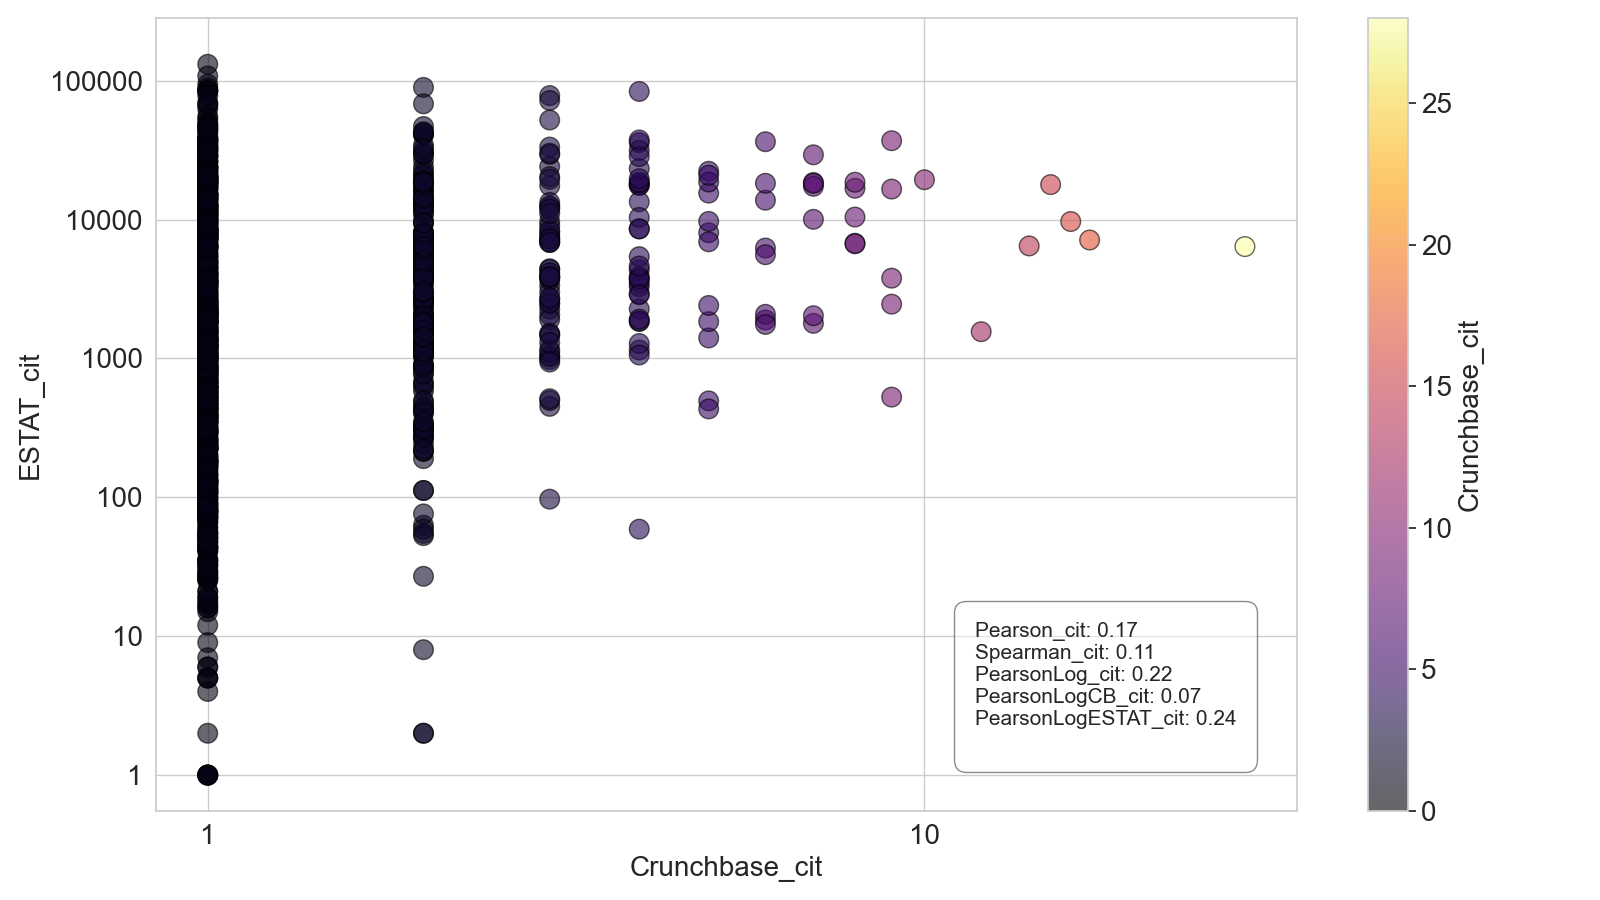
\includegraphics[width=1.0\textwidth]{images/flows/original/ESTAT_cit_False.png}
        \caption{Flussi cittadini}
        \label{fig:estatcrunchfalse_cit}
    \end{subfigure}
    \begin{subfigure}{\textwidth}
        \centering
        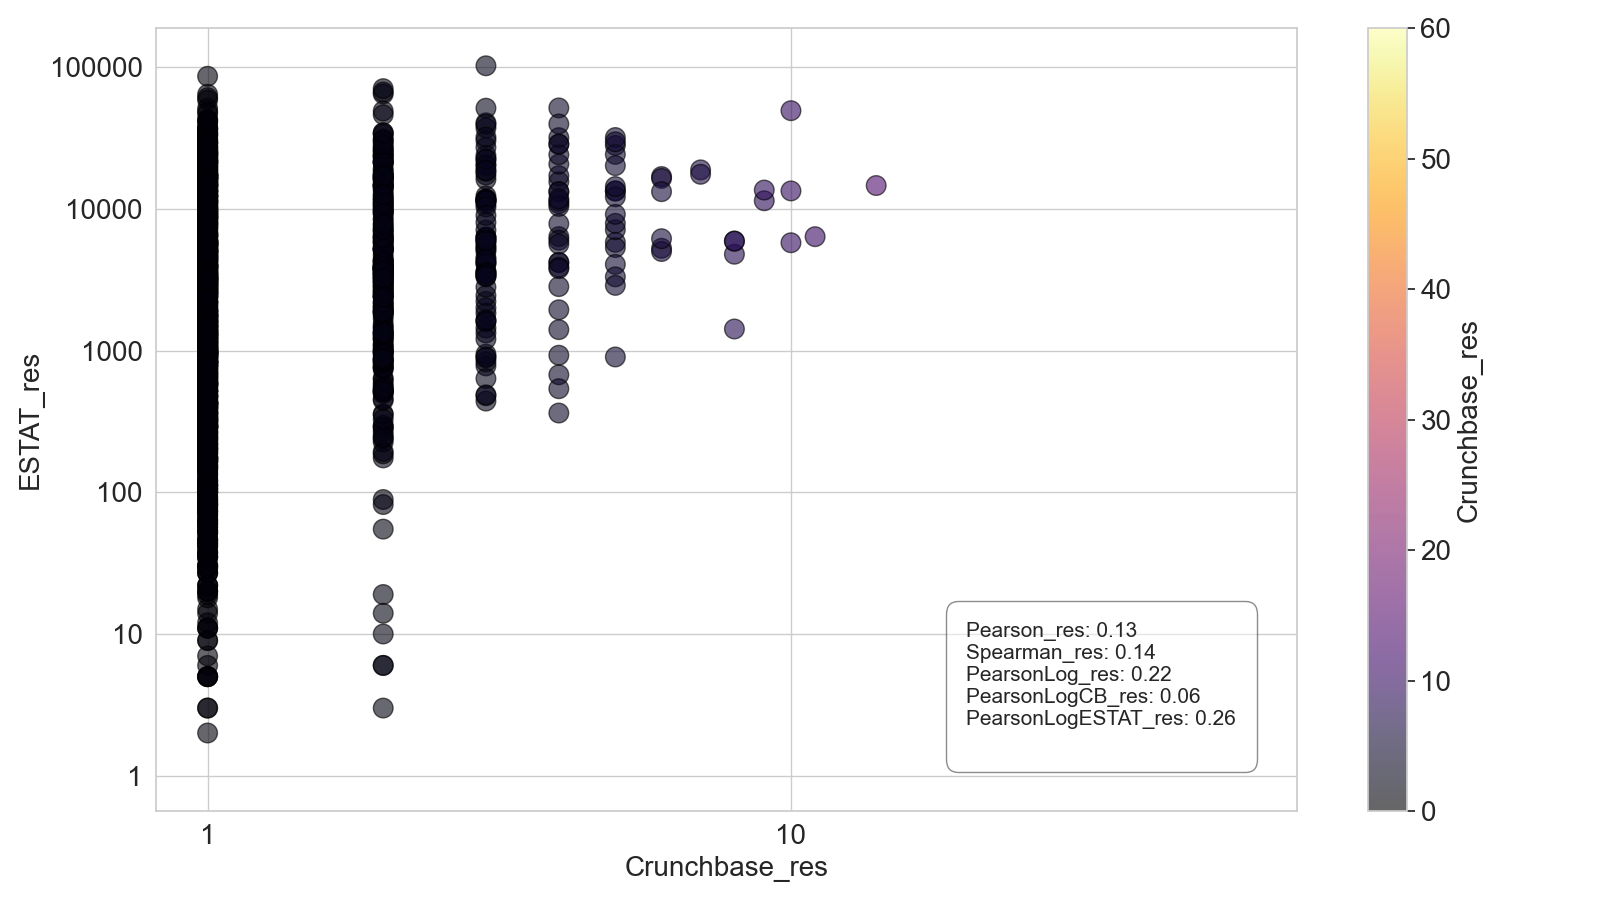
\includegraphics[width=1.0\textwidth]{images/flows/original/ESTAT_res_False.png}
        \caption{Flussi residenti}
        \label{fig:estatcrunchfalse_res}
    \end{subfigure}
    \caption{Confronto dei flussi Crunchbase con i flussi Eurostat (2010 al 2020).}
    \label{fig:estatcrunchfalse}
\end{figure}
\par 
La Figura \ref{fig:estatcrunchfalse_cit} mostra il confronto tra i flussi di Crunchbase ed di Eurostat per i cittadini che migrano dal paese di nazionalità. La correlazione di Pearson è di 0.17, simile all'indice di Spearman (0.11), indicando una scarsa relazione fra i due set di dati.
Il grafico in Figura \ref{fig:estatcrunchfalse_res} presenta i flussi dei residenti emigranti in Crunchbase e in  Eurostat. Sebbene ci sia un incremento del valore massimo di migranti rispetto al caso dei cittadini, le correlazioni sono molto basse (Pearson 0.13, Spearman 0.14). 
\paragraph{UN}
\label{UN_original}

\begin{figure}[tb]
    \centering
    \begin{subfigure}{\textwidth}
        \centering
        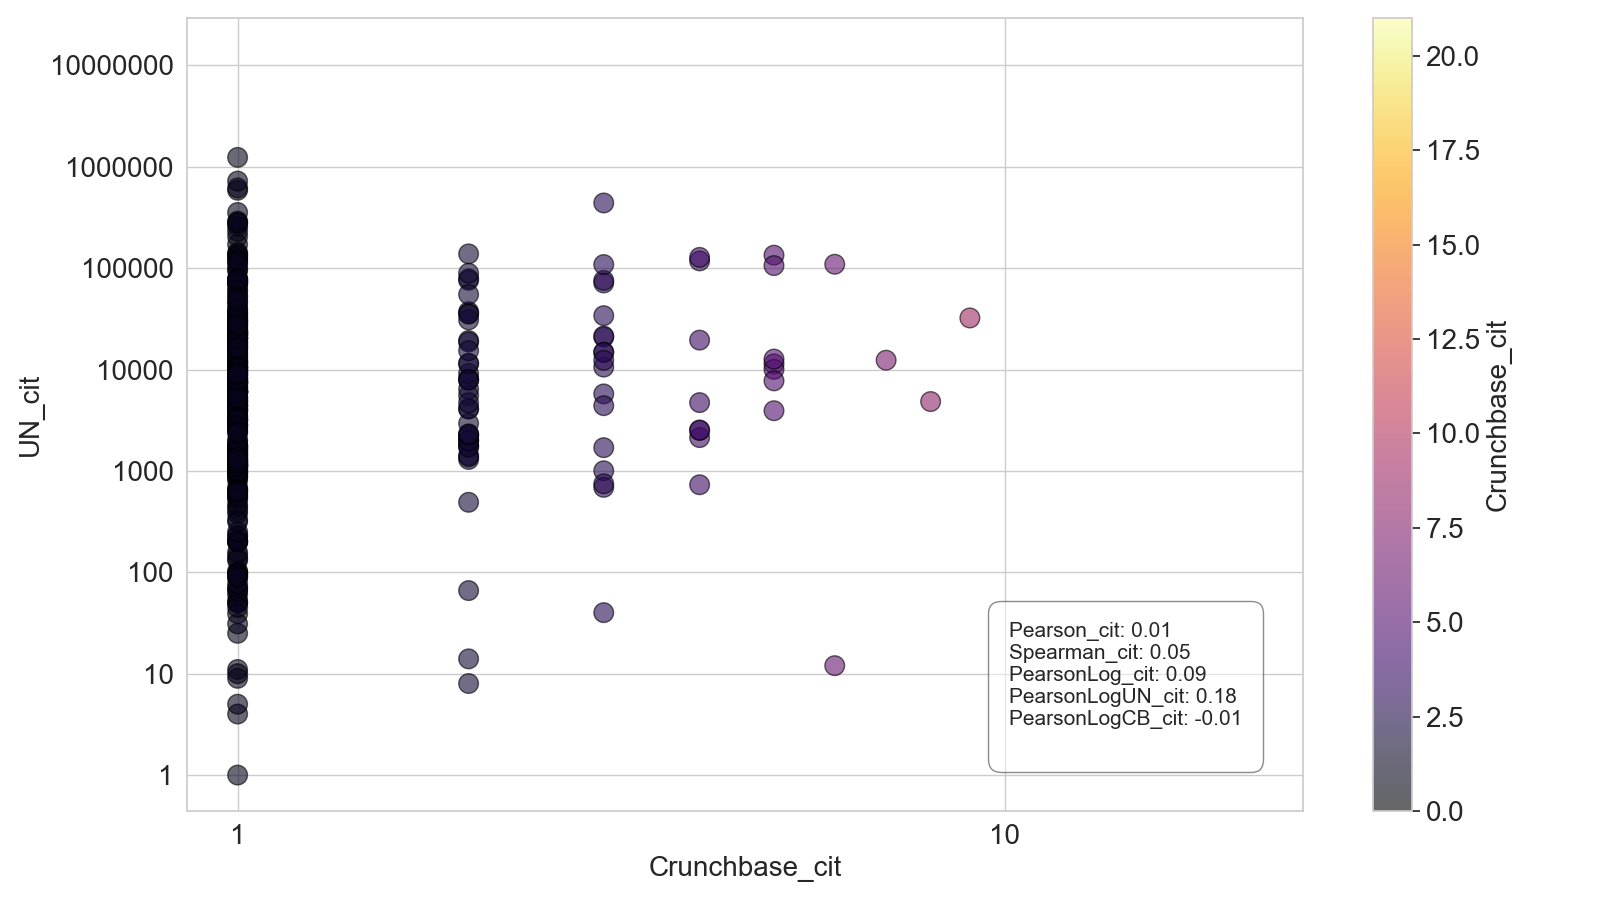
\includegraphics[width=1.0\textwidth]{images/flows/original/UN_cit_False.png}
        \caption{Flussi cittadini}
        \label{fig:uncrunchfalse_cit}
    \end{subfigure}
    \begin{subfigure}{\textwidth}
        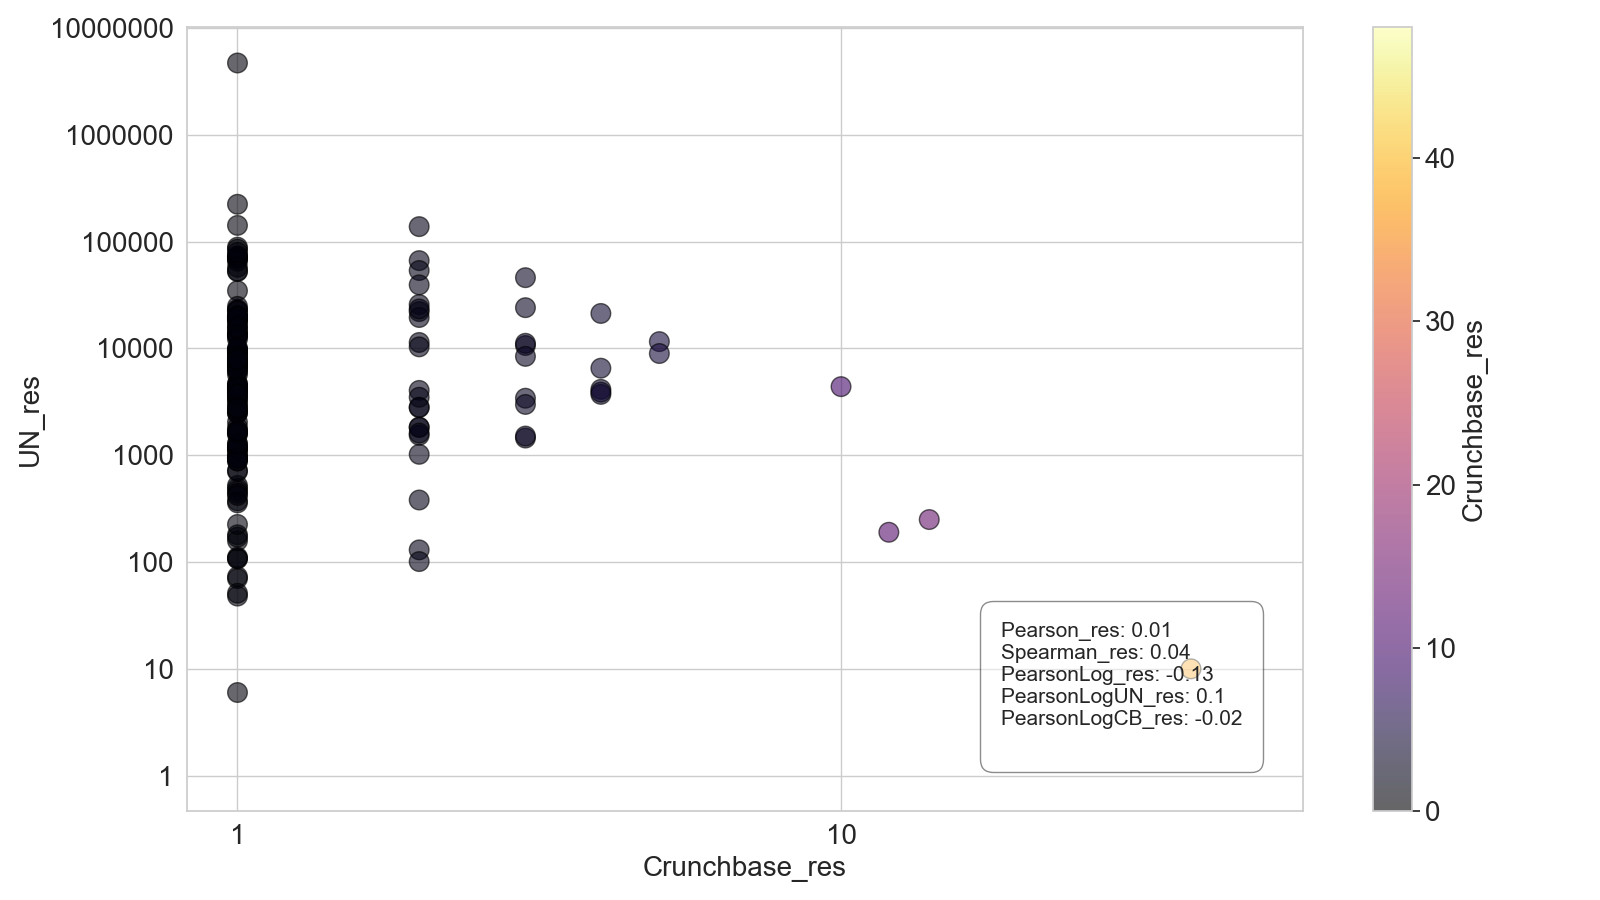
\includegraphics[width=1.0\textwidth]{images/flows/original/UN_res_False.png}
        \caption{Flussi residenti}
        \label{fig:uncrunchfalse_res}
    \end{subfigure}
    \caption{Confronto dei flussi in Crunchbase con UN dal 2010 al 2020.}
    \label{fig:uncrunchfalse}
\end{figure}
La Figura \ref{fig:uncrunchfalse_cit} mostra i flussi dei cittadini che hanno migrato in confronto a UN. La Figura \ref{fig:uncrunchfalse_res} mostra i flussi dei residenti. Entrambi i casi non presentano correlazione per Pearson e Spearman. Il valore massimo di flussi di migranti per Crunchbase in confronto a UN non supera le 40 unità. 
Il confronto dei dati relativi ai flussi di Crunchbase con i flussi di UN (Sezione \ref{UN_original}) ed i flussi di Eurostat (Sezione \ref{ESTAT_original}) non ha mostrato correlazioni significative.
\FloatBarrier

\subsection{Confronto UN ed Eurostat con stati aggregati}
\paragraph{Eurostat con stati aggregati}
Analizziamo i flussi Crunchbase aggregando (sommando) i flussi degli stati per zone geografiche.
L'analisi di dati aggregati porta ad avere informazioni meno specifiche per gli stati in dettaglio, ma permette di comprendere quali sono le zone più interessate dai flussi in ingresso ed in uscita.
\label{ESTAT_aggregated}
\begin{figure}[!ht]
    \centering
    \begin{subfigure}{\textwidth}
        \centering
        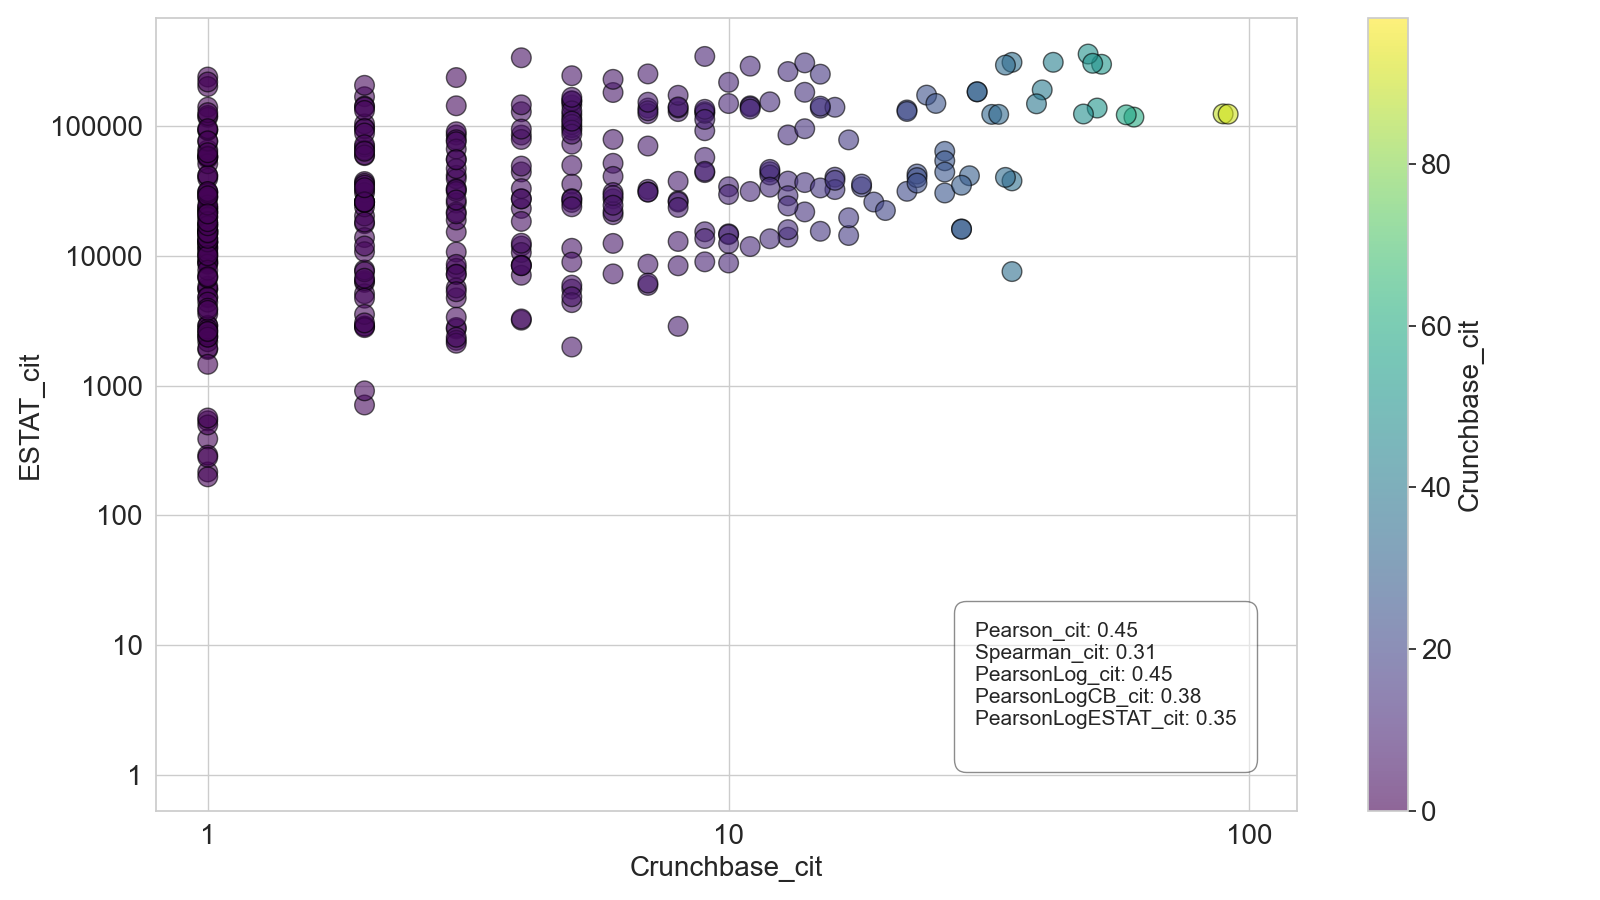
\includegraphics[width=0.95\textwidth]{images/flows/aggregated/ESTAT_cit_True.png}
        \caption{Flussi cittadini}
        \label{fig:estatcrunchtrue_cit}
    \end{subfigure}
    \begin{subfigure}{\textwidth}
        \centering
        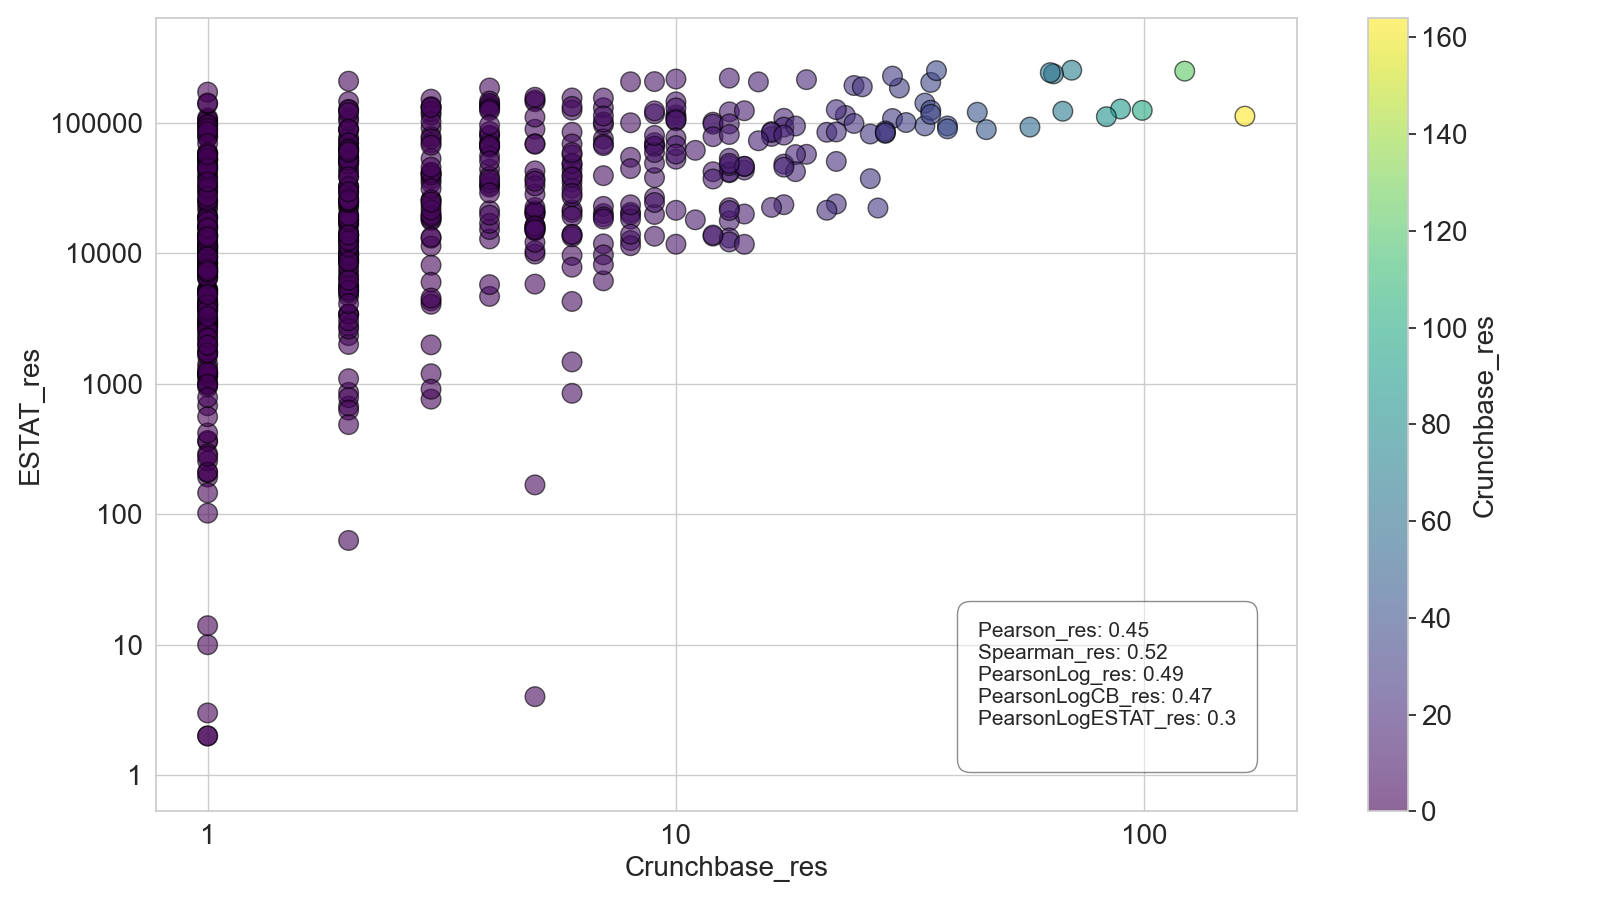
\includegraphics[width=0.95\textwidth]{images/flows/aggregated/ESTAT_res_True.png}
        \caption{Flussi residenti}
        \label{fig:estatcrunchtrue_res}
    \end{subfigure}
    \caption{Confronto dei flussi Crunchbase con i flussi in Eurostat aggregati per zone geografiche dal 2010 al 2020}
    \label{fig:estatcrunchtrue}
\end{figure}
Nella Figura \ref{fig:estatcrunchtrue_cit} viene mostrato il grafico di confronto tra Eurostat e Crunchbase dei cittadini emigrati aggregati per zone geografiche, dal 2010 al 2020.
La correlazione di Pearson è di 0.45, a differenza dell'indice di Spearman che indica un valore di 0.31. Il coefficiente  di Pearson suggerisce che esista una correlazione debole tra i dati dei flussi aggregati di Crunchbase e UN.


La Figura \ref{fig:estatcrunchtrue_res} mostra il confronto tra Eurostat e Crunchbase dei residenti migrati aggregati per zone geografiche. La correlazione di Pearson (0.45) indica una correlazione debole, l'indice di Spearman (0.52) invece indica una correlazione discreta. La correlazione di Pearson calcolata con i flussi Crunchbase in scala logaritmica ottiene un valore superiore (0.47) alla correlazione normale, ma pur sempre basso.

\paragraph{UN con stati aggregati}
\label{UN_aggregated}
\begin{figure}[tb]
    \centering
    \begin{subfigure}{\textwidth}
        \centering
        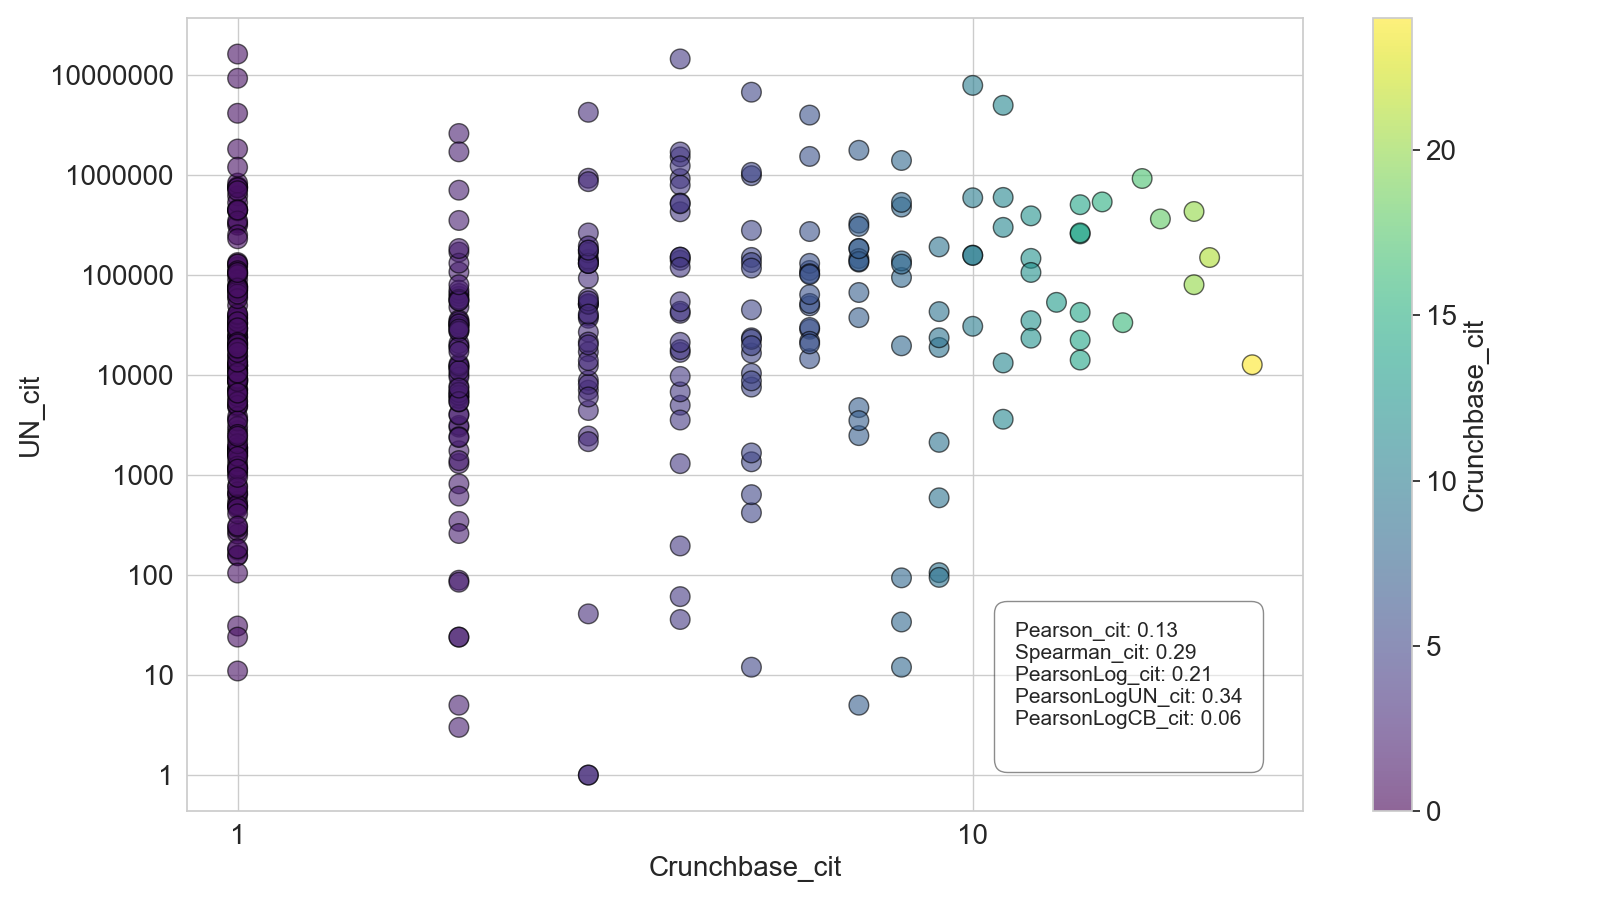
\includegraphics[width=0.95\textwidth]{images/flows/aggregated/UN_cit_True.png}
        \caption{Flussi cittadini}
        \label{fig:uncrunchtrue_cit}
    \end{subfigure}
    \begin{subfigure}{\textwidth}
        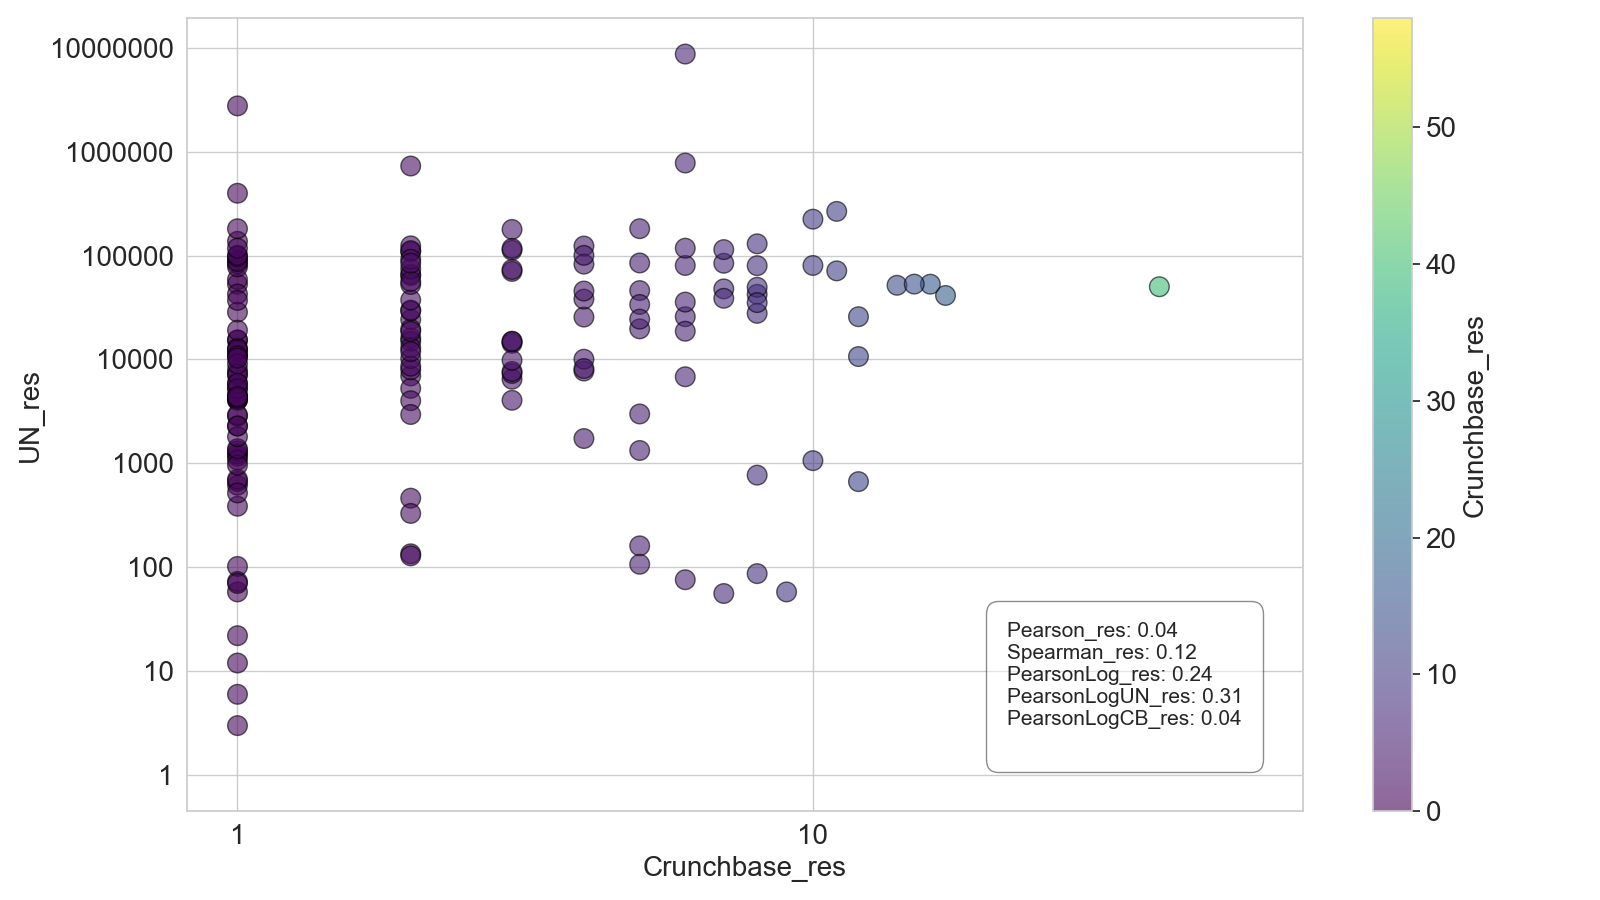
\includegraphics[width=0.95\textwidth]{images/flows/aggregated/UN_res_True.png}
        \caption{Flussi residenti}
        \label{fig:uncrunchtrue_res}
    \end{subfigure}
    \caption{Confronto dei flussi Crunchbase con i flussi in UN aggregati per zone geografiche dal 2010 al 2020.}
    \label{fig:uncrunchtrue}
\end{figure}
In Figura \ref{fig:uncrunchtrue_cit} vengono mostrati i flussi dei cittadini aggregati per zone geografiche in UN e Crunchbase. Il confronto presenta una correlazione di Pearson di 0.13 ed un indice di Spearman di 0.29. Il valore della correlazione di Pearson è di 0.34 utilizzando una scala logaritmica per i soli flussi dei cittadini in UN. 
Nella Figura \ref{fig:uncrunchtrue_res} sono presenti i flussi dei residenti aggregati per zone geografiche in UN e Crunchbase. La correlazione di Pearson ha un valore di 0.04 e l'indice di Spearman è di 0.12.
I flussi migratori di UN sono più significativi per il sudest asiatico, come visto in \cite{MIMIDOC}. Come vediamo nell'analisi del flussi di Crunchbase (Sezione \ref{flowscrunch}), il sudest asiatico non è rappresentato.
Nel caso dei cittadini i risultati indicano una correlazione bassa ponendo i dati Crunchbase in scala logaritmica. Di contro, i risultati ottenuti per il confronto dei residenti indicano che non ci sia correlazione.

\FloatBarrier
\subsection{Flussi aggregati UN unito Eurostat}
\label{UNunionEstatflows}
Per questo studio i dati di Crunchbase sono stati confrontati con l'unione di UN ed Eurostat, aggregando gli stati per zona geografica. Per l'unione dei due dataset (UN e Eurostat) è stato selezionato, per ogni paese, il flusso di maggior valore tra i due insiemi. Il periodo è come negli altri casi di studio dal 2010 al 2020.
Il grafico nella Figura \ref{fig:off_true_cit} rappresenta i cittadini. La correlazione di Pearson è di 0.06, mentre l'indice di Spearman è di 0.38. Con i dati ufficiali in scala logaritmica si ha una correlazione di Pearson di 0.24. I valori del coefficiente di Pearson indicano che non sia presente correlazione, a differenza dell'indice di Spearman che determina una correlazione debole.
Nella Figura \ref{fig:off_true_res} riferita ai residenti si ottiene una correlazione di Pearson di 0.08 e un indice di Spearman di 0.37. Con i dati ufficiali in scala logaritmica si ha una correlazione di Pearson di 0.27. Come per i cittadini questo confronto ha correlazione debole per Spearman. Inoltre, i valori ottenuti sono inferiori rispetto all'analisi effettuata con i soli dati Eurostat aggregati (Sezione \ref{ESTAT_aggregated}). 

\begin{figure}[ht]
    \begin{subfigure}{\textwidth}
        \centering
        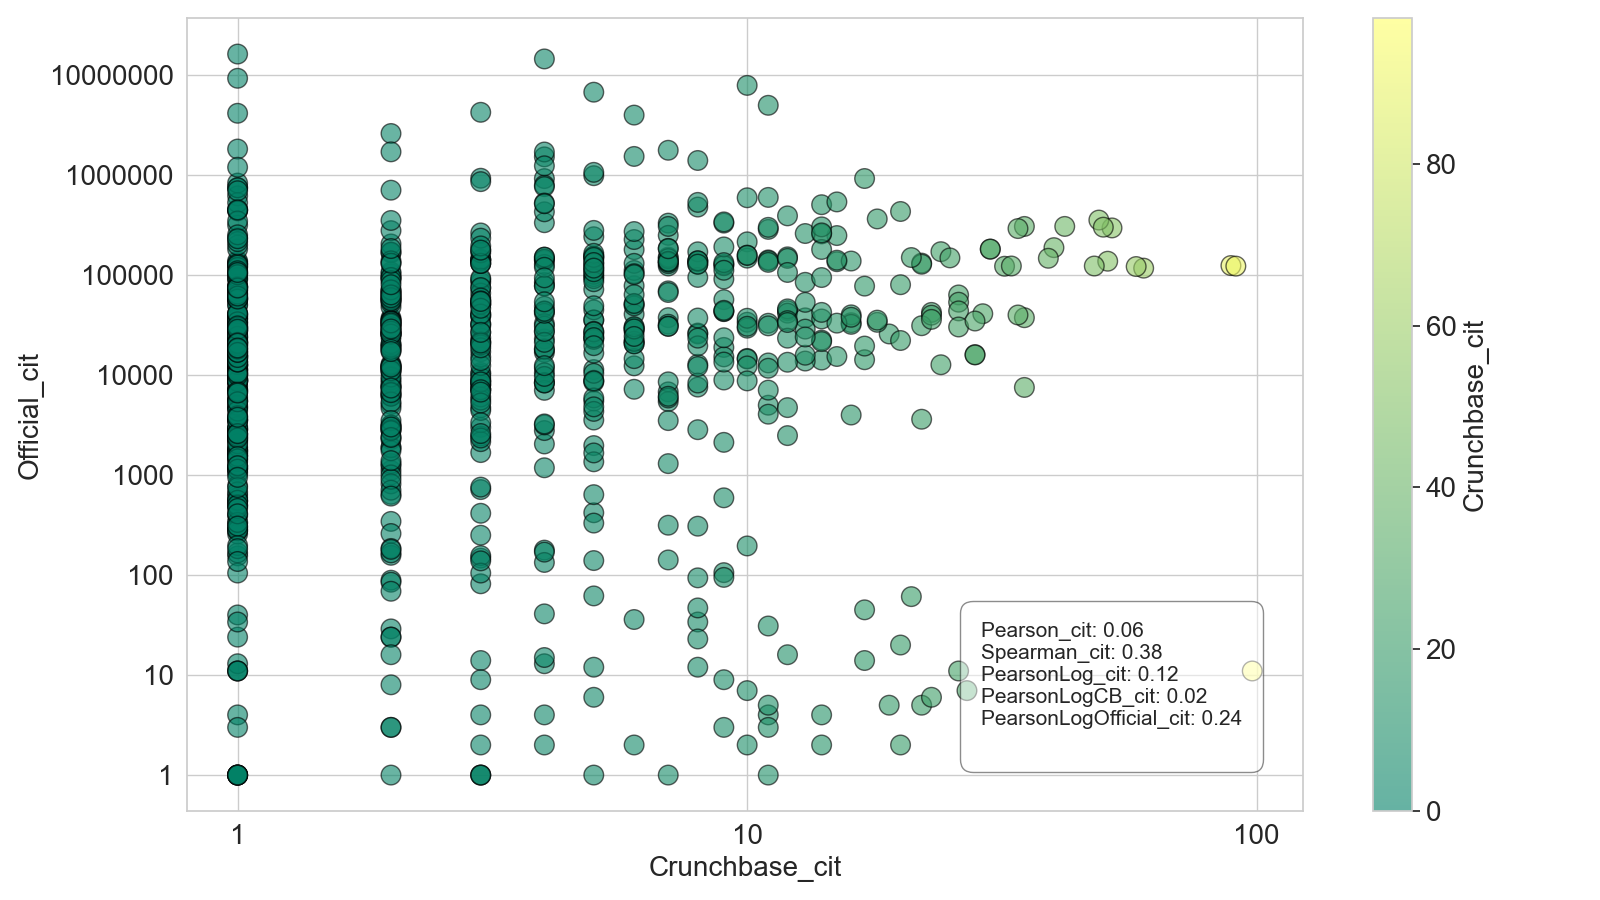
\includegraphics[width=1\textwidth]{images/congiunti/Flows/Official_cit_True.png}
        \caption{Flussi cittadini \(UN\cup{Eurostat}\)}
        \label{fig:off_true_cit}
    \end{subfigure}
\end{figure}
\begin{figure}[tb]\ContinuedFloat
    \begin{subfigure}{\textwidth}
        \centering
        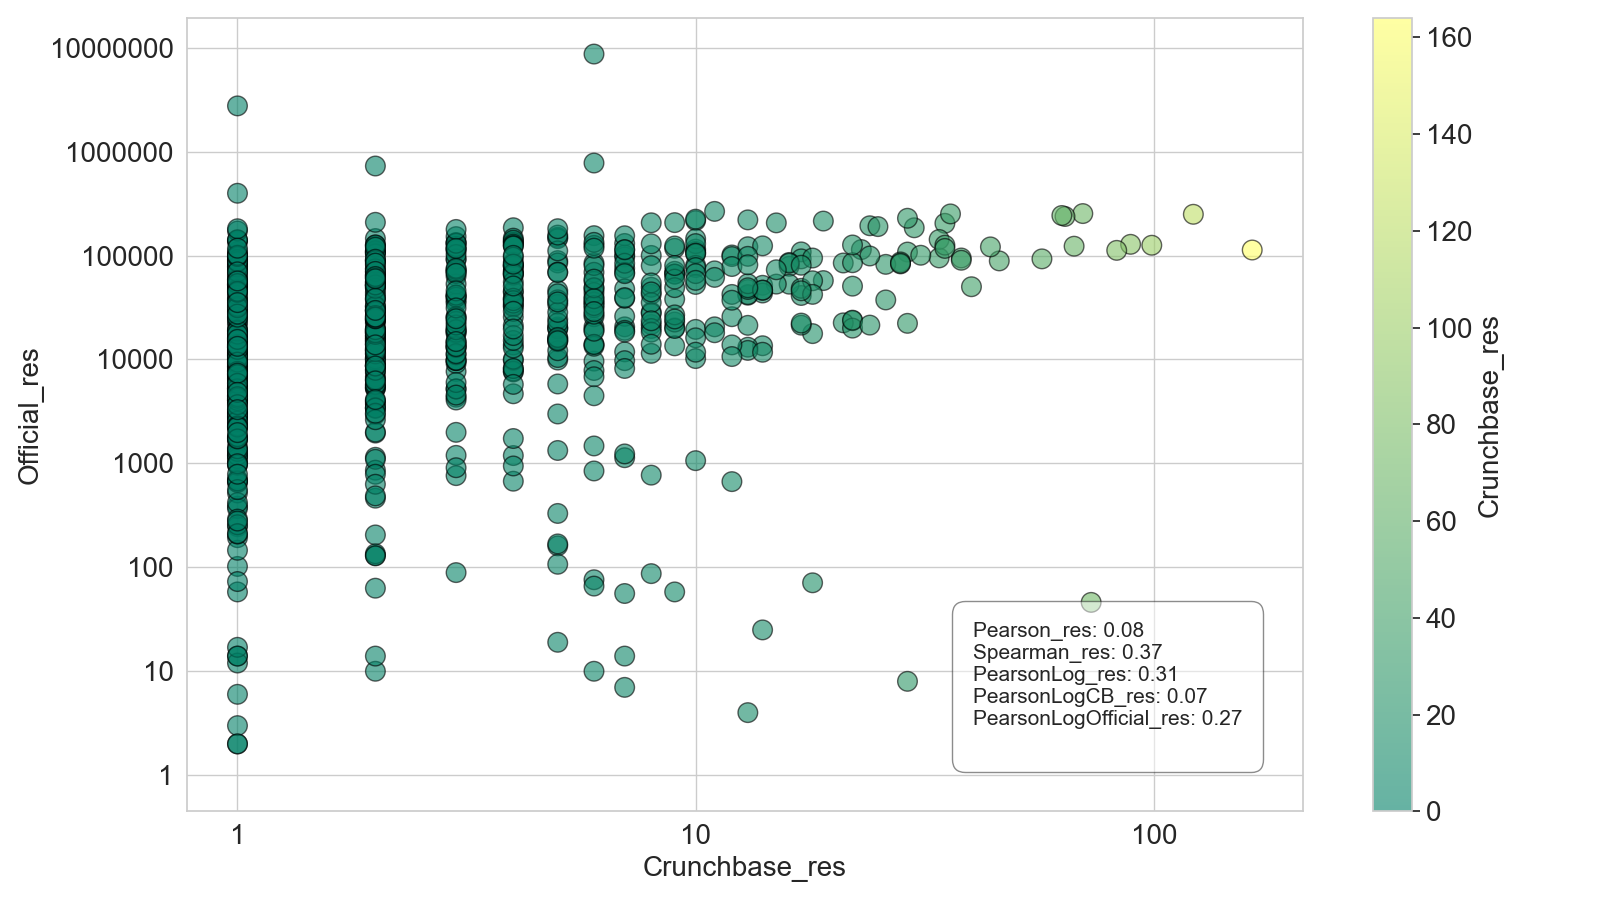
\includegraphics[width=1\textwidth]{images/congiunti/Flows/Official_res_True.png}
        \caption{Flussi residenti \(UN\cup{Eurostat}\)}
        \label{fig:off_true_res}
    \end{subfigure}
    \caption{Confronto dei flussi Crunchbase con i flussi presenti nell'unione di UN ed ESTAT (stati aggregati per zone geografiche dal 2010 al 2020.}
    \label{fig:off_true}
\end{figure}

\FloatBarrier

\subsection{Caso di studio: Italia}
In questa sezione vengono analizzati i flussi d'immigrazione ed emigrazione, di residenti e cittadini, che interessano l'Italia. Il periodo dell'analisi è riferito al periodo dell'insieme di dati collezionati (dal 2010 al 2020), ed il dataset di confronto è quello Eurostat.
\paragraph{Flussi di emigranti dall'Italia}
\label{ita_flows}
\begin{figure}[tb]
    \centering
    \begin{subfigure}{\textwidth}
        \centering
        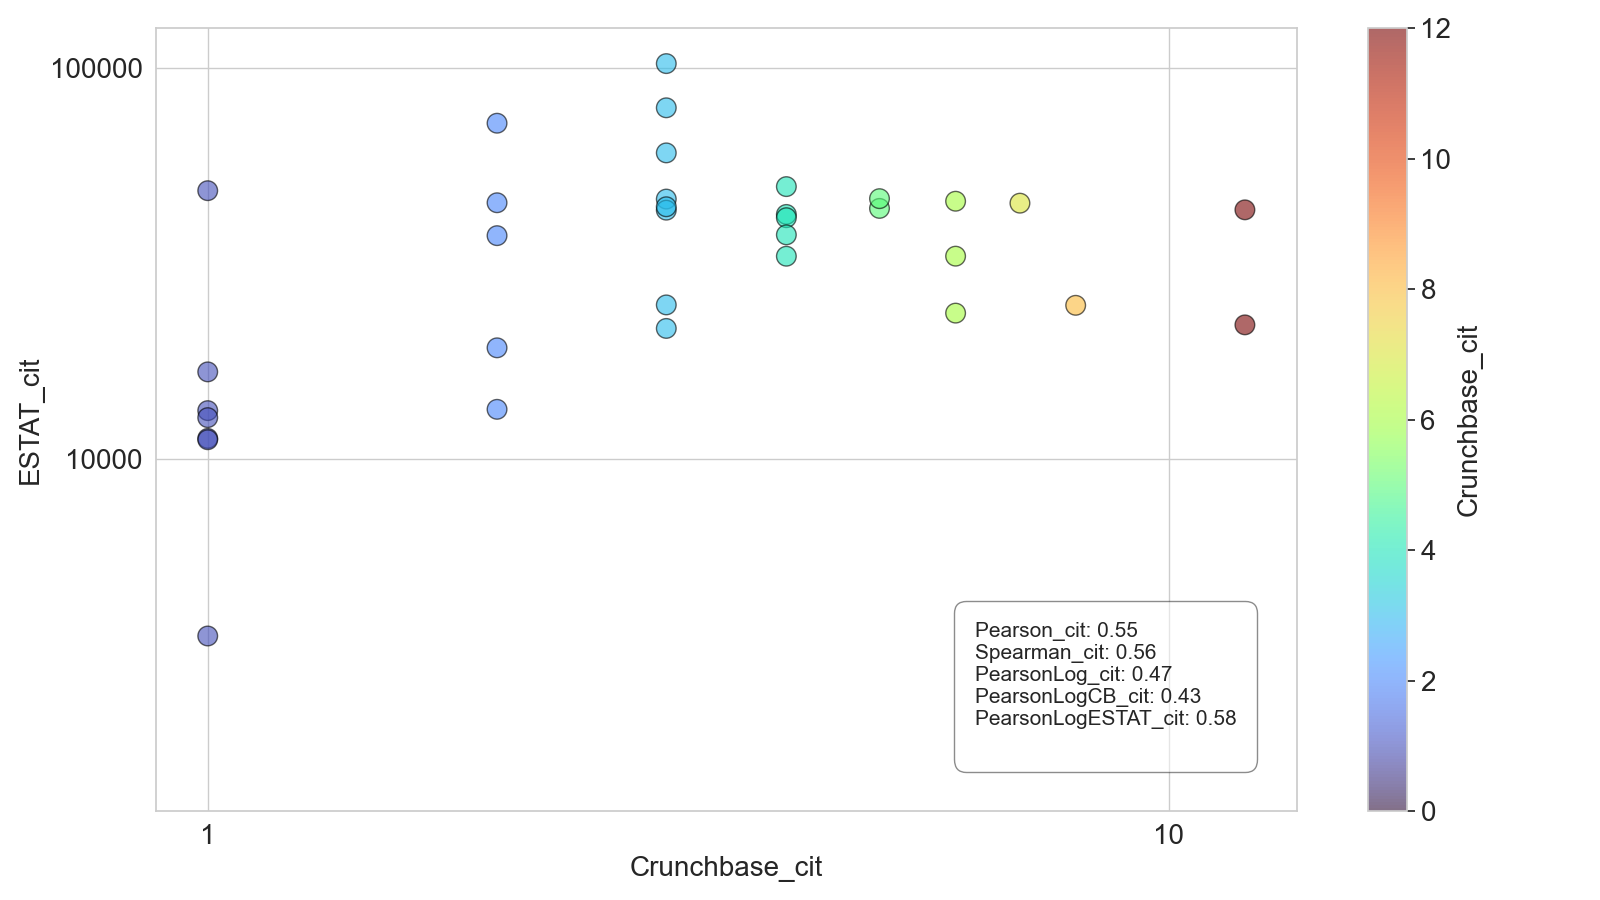
\includegraphics[width=1.0\textwidth]{images/flows/aggregated/filtered_nationality/ita/ESTAT_cit_True.png}
        \caption{Flussi cittadini}
        \label{fig:italia_nat_true}
    \end{subfigure}
    \begin{subfigure}{\textwidth}
        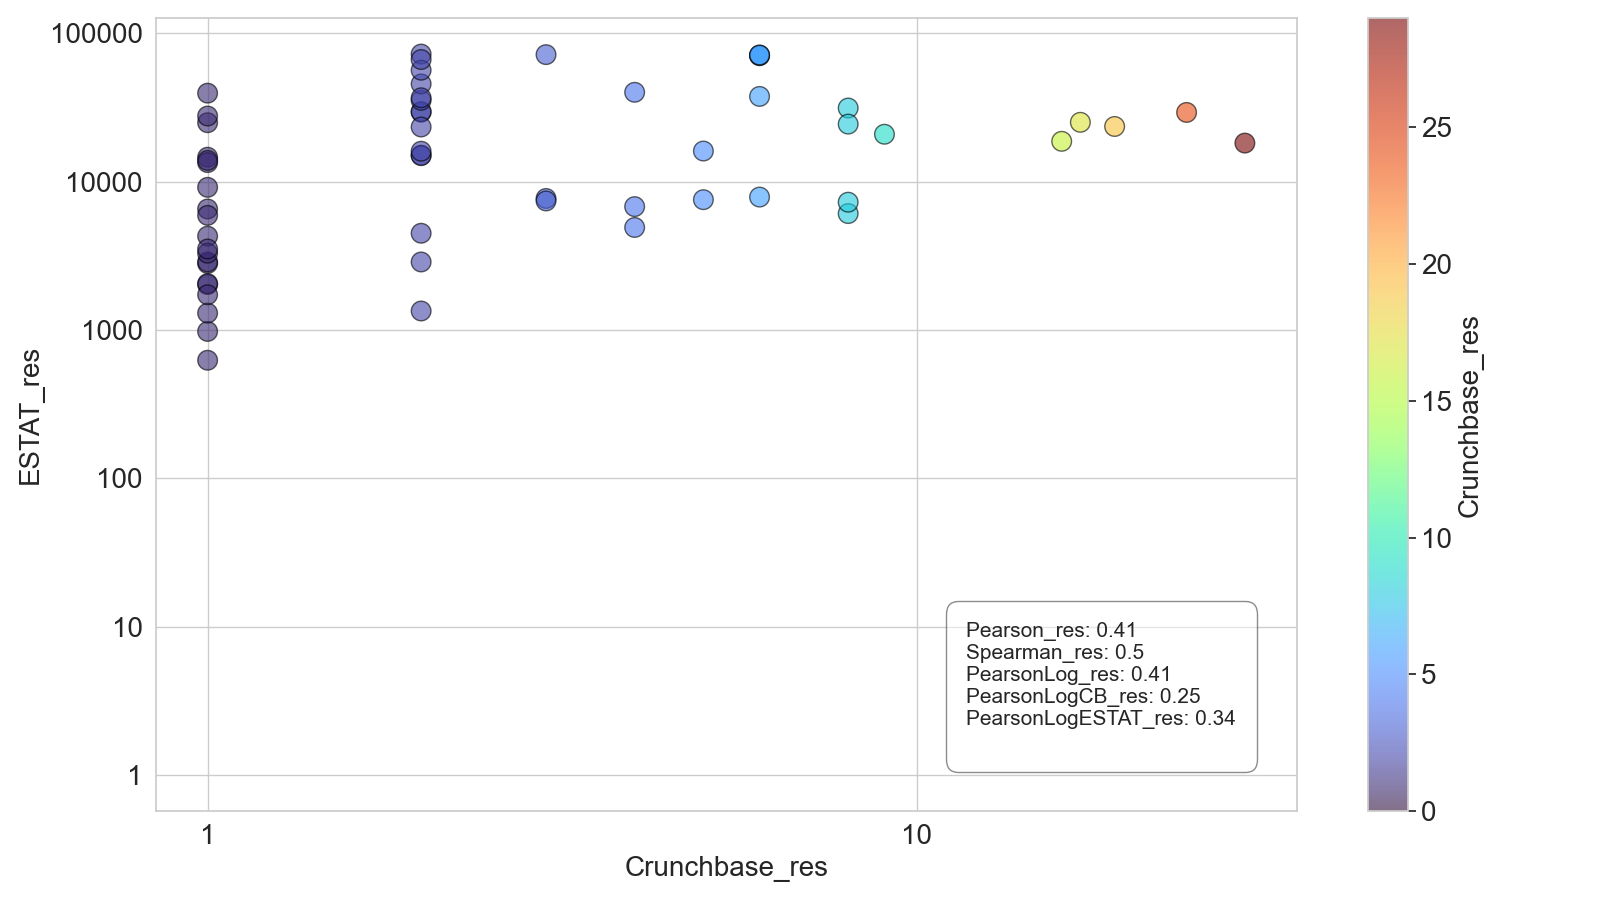
\includegraphics[width=1.0\textwidth]{images/flows/aggregated/filtered_nationality/ita/ESTAT_res_True.png}
        \caption{Flussi residenti}
        \label{fig:italia_res_true}
    \end{subfigure}
    \caption{Confronto dei flussi di emigranti, dall'Italia, di Crunchbase con Eurostat (gli altri stati sono aggregati per zone, periodo 2010 al 2020).}
    \label{fig:italiatrue}
\end{figure}
Nella Figura \ref{fig:italia_nat_true} viene mostrato il confronto dei flussi di emigranti di nazionalità Italiana tra Crunchbase ed Eurostat. Gli stati oltre all'Italia vengono aggregati per zona geografica. Si nota una correlazione di Pearson di 0.55, l'indice di Spearman indica un valore di 0.56. Ponendo i soli dati Eurostat in scala logaritmica la correlazione di Pearson ottiene un valore di 0.58.

La Figura \ref{fig:italia_res_true} mostra i flussi migratori dei residenti in Italia. La correlazione di Pearson è di 0.4, invece l'indice di Spearman è di 0.5. Interventi di trasformazione in scala logaritmica di uno dei due insiemi (Eurostat e Crunchbase) portano a correlazioni di Pearson uguali o inferiori (0.41, 0.25, 0.34).

Entrambi i casi di confronto indicano una correlazione discreta tra i flussi di Crunchbase ed Eurostat per gli utenti emigrati dall'Italia. Si nota dalla barra laterale come il valore massimo di emigranti altamente qualificati dall'Italia nei flussi Crunchbase è intorno alle 25 unità. 

\paragraph{Flussi d'immigrazione in Italia}
\label{toIta_flows}
\begin{figure}[tb]
    \centering
    \begin{subfigure}{\textwidth}
        \centering
        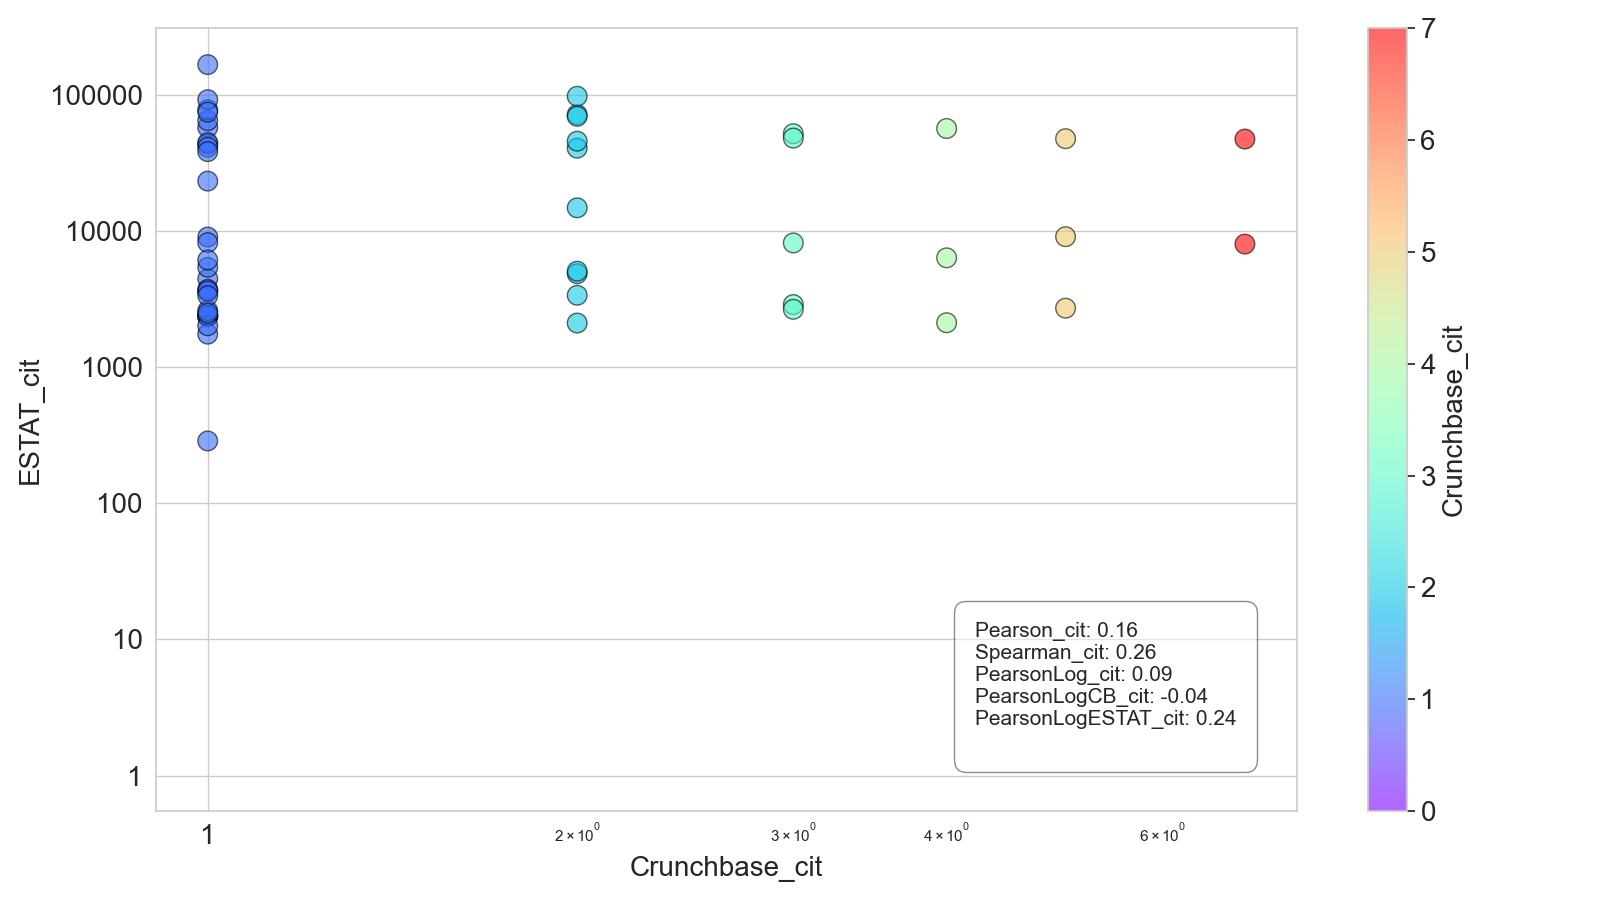
\includegraphics[width=1.0\textwidth]{images/flows/aggregated/filtered_destination/ita/ESTAT_cit_True.png}
        \caption{Flussi cittadini}
        \label{fig:italia_dest_true_cit}
    \end{subfigure}
    \begin{subfigure}{\textwidth}
        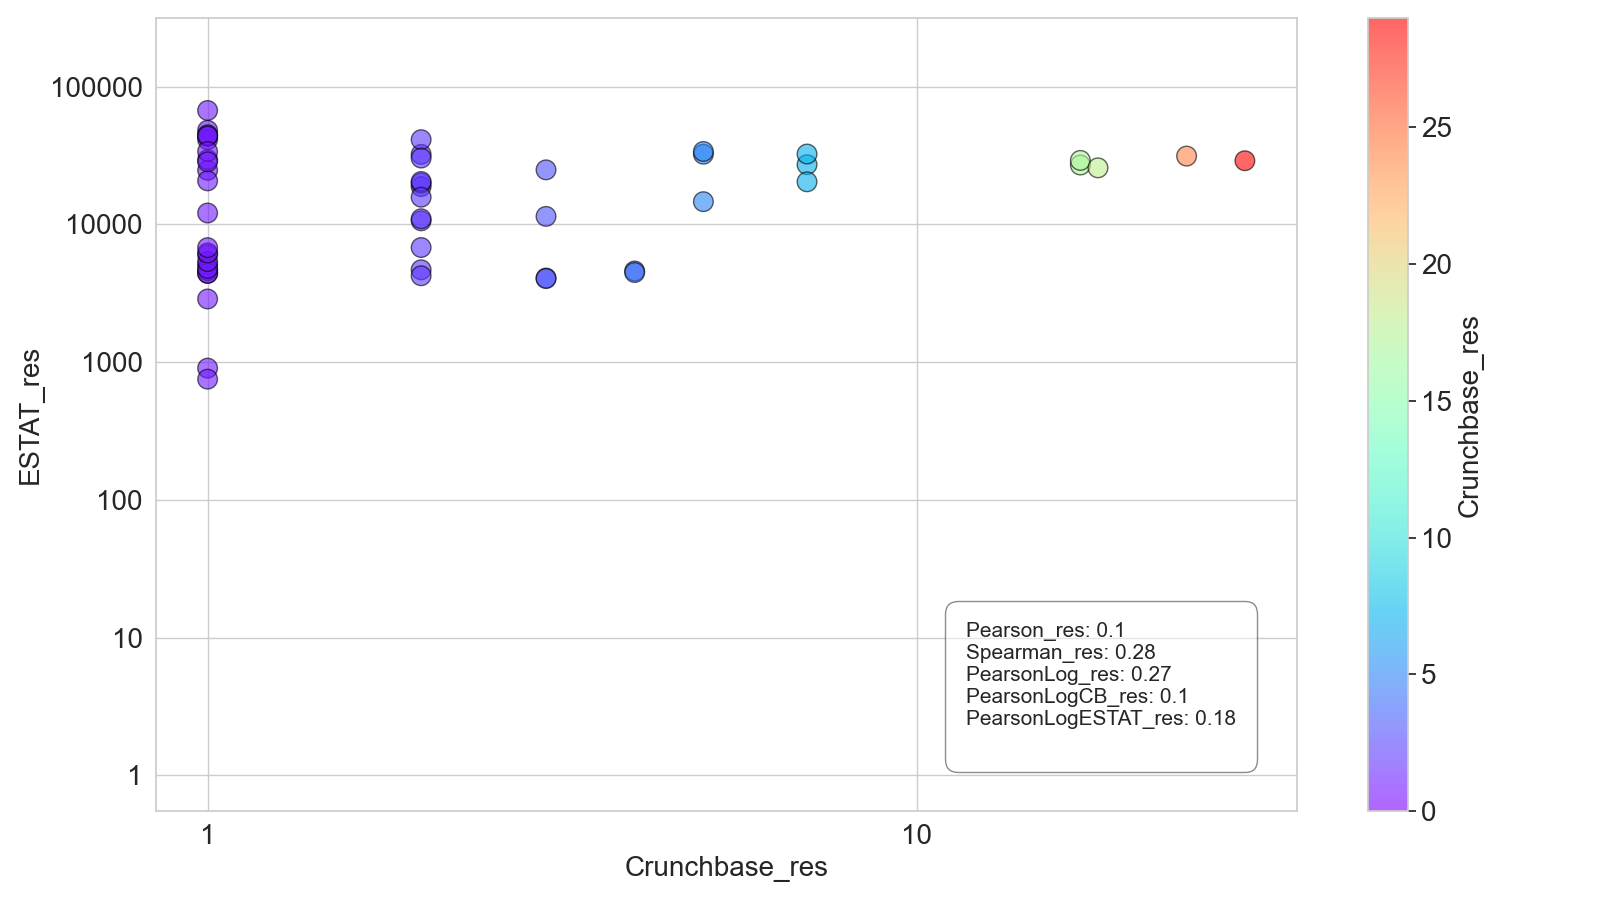
\includegraphics[width=1.0\textwidth]{images/flows/aggregated/filtered_destination/ita/ESTAT_res_True.png}
        \caption{Flussi residenti}
        \label{fig:italia_dest_true_res}
    \end{subfigure}
    \caption{Confronto dei flussi di immigranti in Italia, tra Crunchbase ed Eurostat (gli altri stati sono aggregati per zone, periodo 2010 al 2020).}
\end{figure}
Nella Figura \ref{fig:italia_dest_true_cit} viene mostrato il flusso di cittadini esteri che hanno migrato in Italia. 
La correlazione di Pearson è di 0.16, l'indice di Spearman è di 0.26. Ponendo in scala logaritmica i flussi dei cittadini in Eurostat la correlazione di Pearson incrementa fino a 0.24. Il valore massimo di flussi di cittadini esteri immigrati in Italia incontrato in Crunchbase è di 7 persone. 
In Figura \ref{fig:italia_dest_true_res} è presente il grafico dei flussi dei residenti all'estero che hanno migrato in Italia. Il valore della correlazione di Pearson è di 0.01, ed incrementa fino a 0.18 se poniamo i flussi di Eurostat in scala logaritmica. L'indice di Spearman ha invece un valore di 0.18. Il valore massimo di residenti all'estero immigrati in Italia in Crunchbase è di poco più di 25 persone. Inoltre, i valori dei coefficienti di Pearson e di Spearman per cittadini e residenti indicano che non vi è correlazione tra i dati Crunchbase ed i dati Eurostat per questo caso di studio.

\FloatBarrier

\subsection{Caso di studio: Gran Bretagna}
\label{CASOFLUSSIGBR}
In questa sezione si analizzano in particolare i flussi di migranti da e verso la Gran Bretagna su tutto il periodo dei dati collezionati (dal 2010 al 2020). Il confronto viene fato con i dati ottenuti da UN unito ad Eurostat.
\paragraph{Flussi di emigranti dalla Gran Bretagna}
\label{gbr_flows}
\begin{figure}[!ht]
    \centering
    \begin{subfigure}{\textwidth}
        \centering
        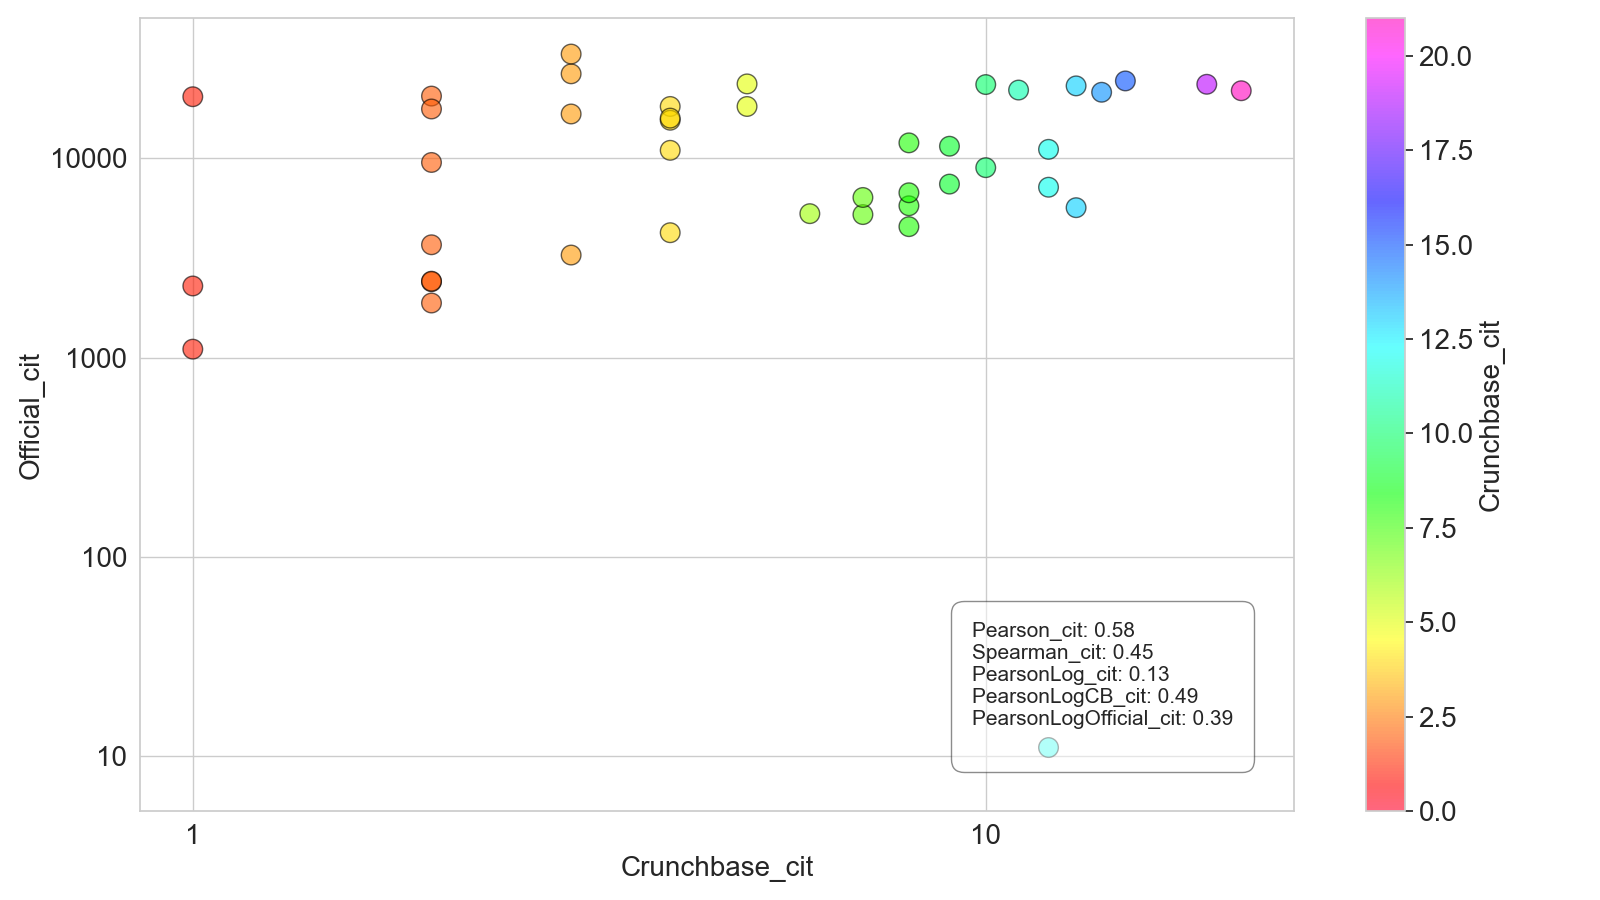
\includegraphics[width=0.95\textwidth]{images/flows/aggregated/filtered_nationality/gbr/Official_cit_True.png}
        \caption{Flussi cittadini}
        \label{fig:gbr_nat_true}
    \end{subfigure}
    \begin{subfigure}{\textwidth}
        \centering
        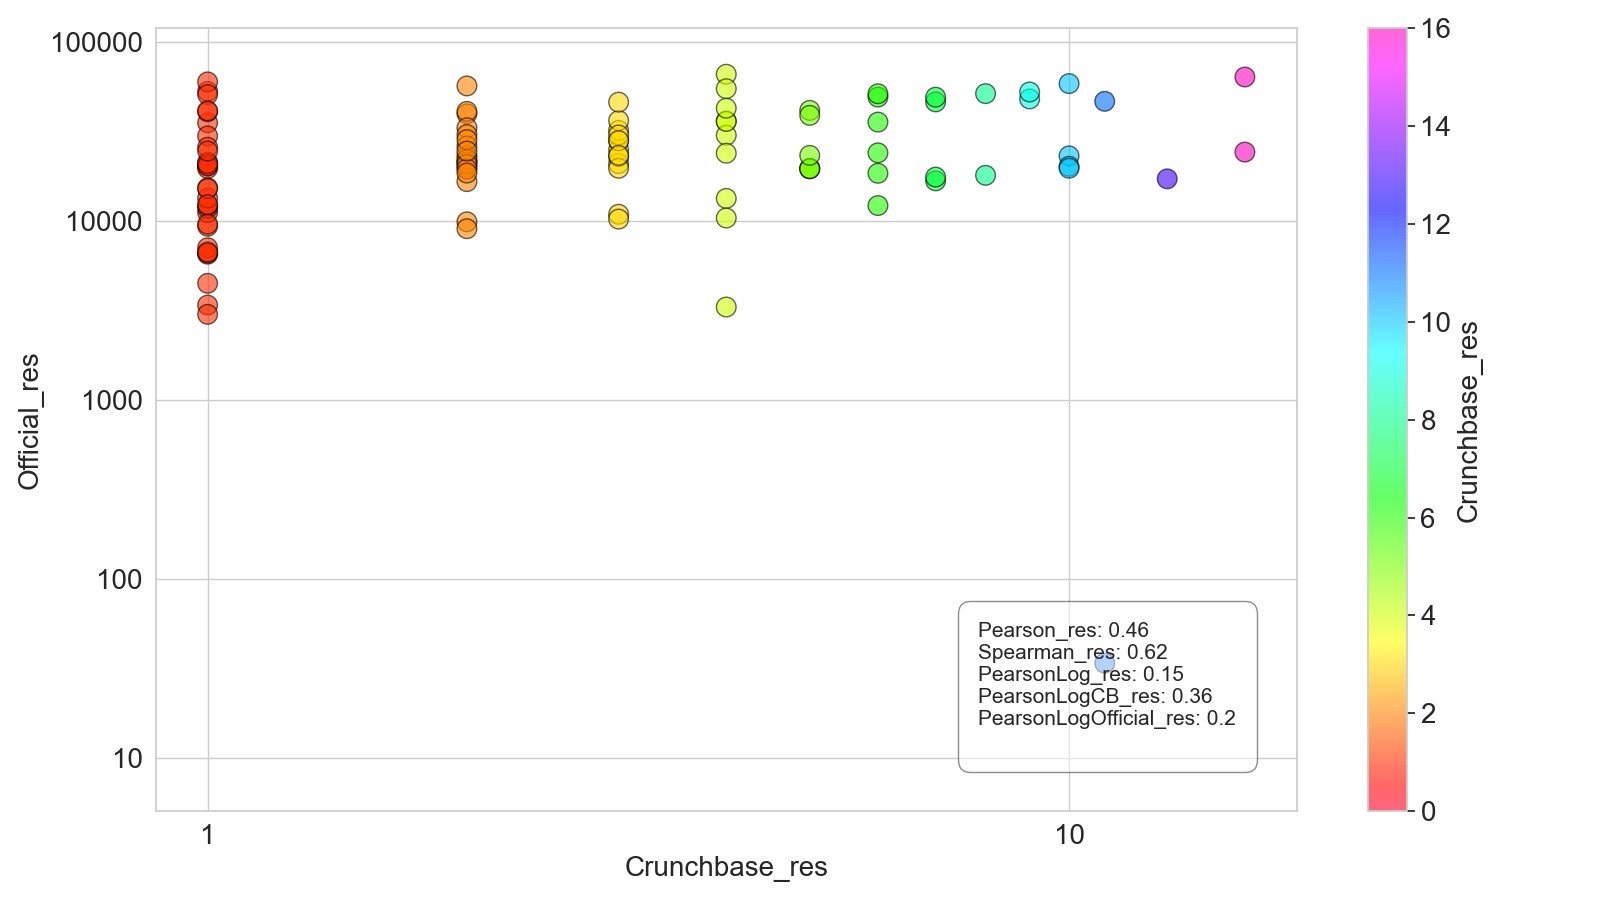
\includegraphics[width=0.95\textwidth]{images/flows/aggregated/filtered_nationality/gbr/Official_res_True.png}
        \caption{Flussi residenti}
        \label{fig:gbr_res_true}
    \end{subfigure}
    \caption{Confronto dei flussi di emigranti britannici, tra Crunchbase e UN unito Eurostat (gli altri stati sono aggregati per zone geografiche, il periodo è 2010-2020).}
    \label{fig:gbr_True}
\end{figure}
In Figura \ref{fig:gbr_nat_true} viene mostrato il confronto tra i flussi dei cittadini britannici che emigrano, tra  Crunchbase e UN unito Eurostat. 
La correlazione di Pearson ottenuta è di 0.58, invece l'indice di Spearman ha un valore di 0.45. Ponendo gli insiemi in scale logaritmiche la correlazione di Pearson decrementa il suo valore in tutti i casi (0.13, 0.49, 0.39). 
Il grafico in Figura \ref{fig:gbr_res_true} mostra i flussi dei residenti in Gran Bretagna, che hanno emigrato. La correlazione di Pearson ha un valore di 0.46 come per il grafico dei cittadini in Figura \ref{fig:gbr_nat_true}. L'indice di Spearman ha invece un valore di 0.62. Inoltre, utilizzare scale logaritmiche sui flussi (Ufficiali o di Crunchbase) porta a valori inferiori alla correlazione normale. Entrambi i coefficienti indicano una correlazione discreta tra i dati Crunchbase e UN unito Eurostat sia per nativi che residenti della Gran Bretagna che hanno emigrato.
\paragraph{Flussi d'immigrazione in Gran Bretagna}
\label{togbr_flows}
\begin{figure}[tb]
    \centering
    \begin{subfigure}{\textwidth}
        \centering
        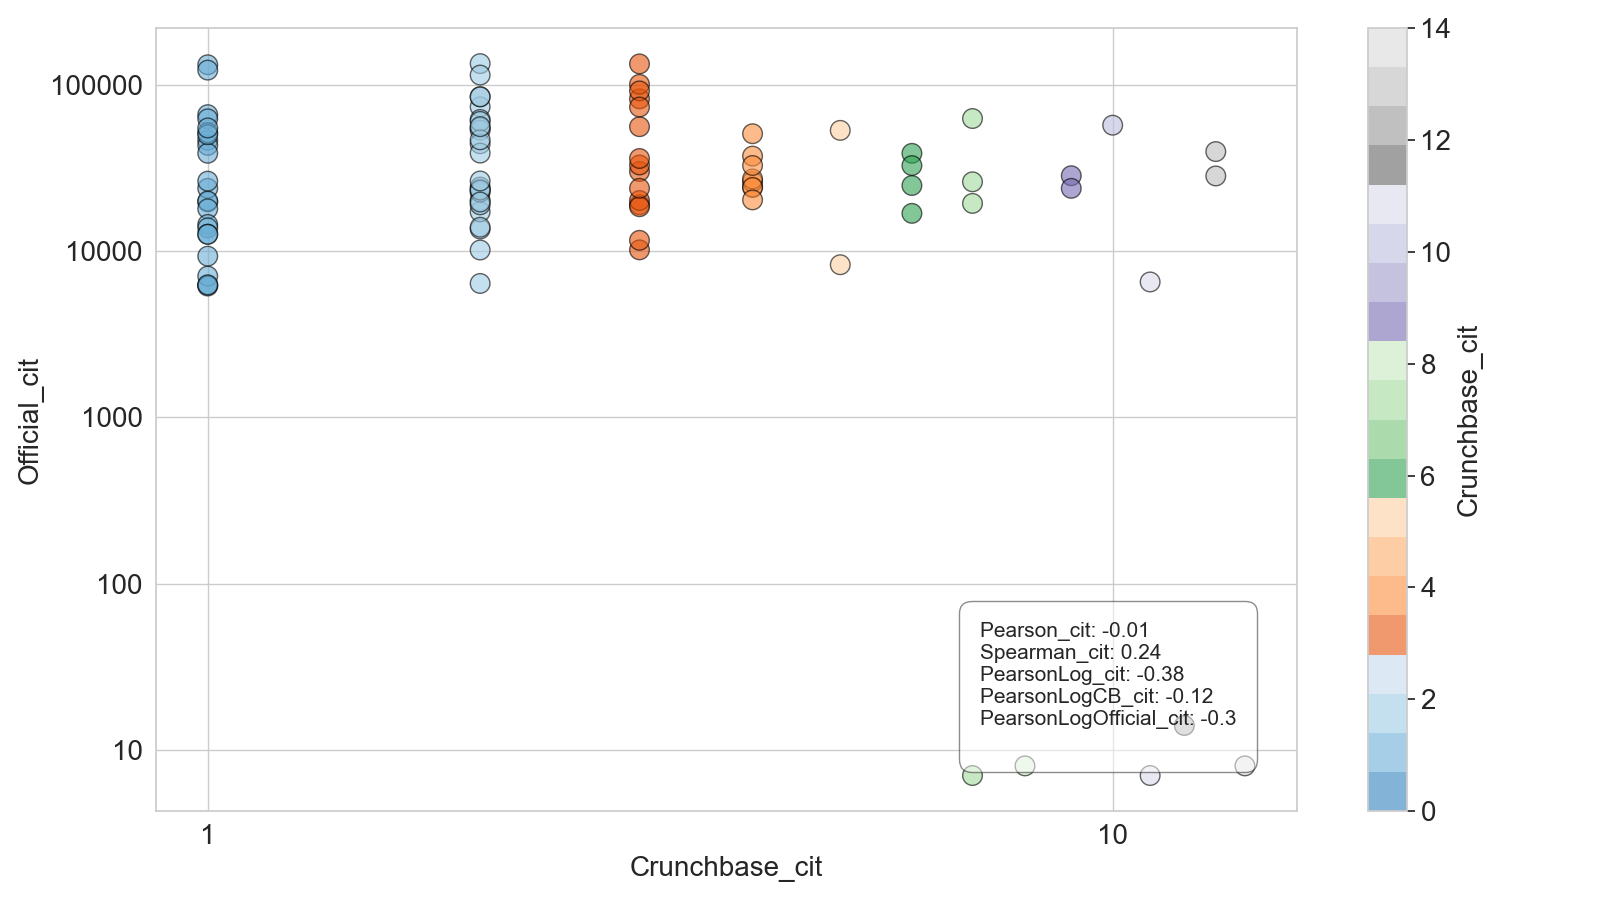
\includegraphics[width=0.9\textwidth]{images/flows/aggregated/filtered_destination/gbr/Official_cit_True.png}
        \caption{Flussi cittadini}
        \label{fig:gbr_dest_true_cit}
    \end{subfigure}
    \begin{subfigure}{\textwidth}
        \centering
        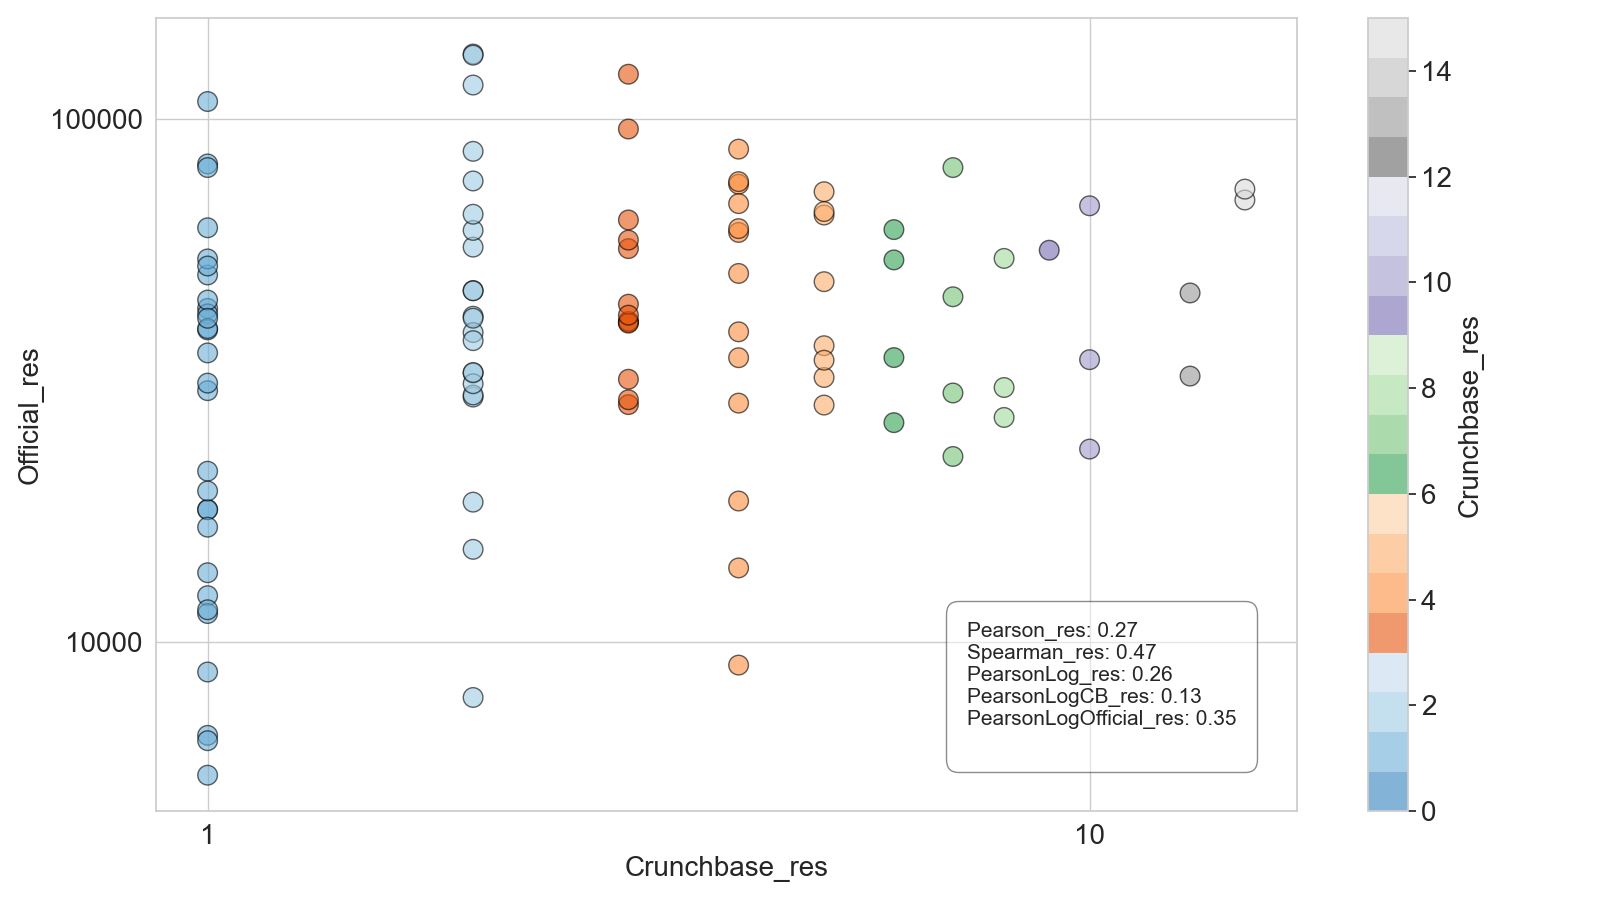
\includegraphics[width=0.9\textwidth]{images/flows/aggregated/filtered_destination/gbr/Official_res_True.png}
        \caption{Flussi residenti}
        \label{fig:gbr_dest_true_res}
    \end{subfigure}
    \caption{Confronto dei flussi di immigranti in Gran Bretagna, tra Crunchbase e UN unito Eurostat (gli altri stati sono aggregati per zone geografiche, il periodo è 2010-2020).}
    \label{fig:gbr_dest_true}
\end{figure}
Nel grafico in Figura \ref{fig:gbr_dest_true_cit} vengono confrontati i flussi di cittadini esteri che migrano in Gran Bretagna, tra Crunchbase e UN unito Eurostat. La correlazione di Pearson è di 0.1, invece l'indice di Spearman ha valore 0.24. Ponendo in scala logaritmica entrambe le fonti dei flussi (UN unito Eurostat e Crunchbase) si ha una correlazione di Pearson negativa di -0.12. Questi valori indicano che non sia presente correlazione tra i dati Crunchbase ed i dati di UN unito Eurostat, per i flussi di cittadini esteri immigrati in Gran Bretagna.
La Figura \ref{fig:gbr_dest_true_res} mostra i flussi degli immigranti in Gran Bretagna. La correlazione di Pearson è di 0.27 l'indice di Spearman è di 0.47. Utilizzando una scala logaritmica per i flussi dei dati ufficiali (UN unito ad Eurostat) si ha una correlazione di Pearson di 0.35.
La correlazione di Spearman indica che ci sia una correlazione positiva discreta tra i dati confrontati.
\FloatBarrier

\subsection{Discussione}
I flussi dei dati collezionati attraverso Crunchbase sono significativi per l'Europa ed il Nord America come visto nella sezione \ref{flowscrunch}. 
La correlazione con i flussi in Eurostat è debole, in alcuni casi anche discreta (Sezione \ref{ESTAT_aggregated}) se aggregati, i flussi in Eurostat però non presentano dati per la Gran Bretagna \cite{MIMIDOC}. 
La correlazione dei flussi con UN non è presente, come abbiamo visto nell'analisi (Sezioni \ref{UN_original}, \ref{UN_aggregated}). 
L'unione dei flussi UN con i flussi Eurostat non ha correlazione per Pearson nell'analisi effettuata, ma per l'indice di Spearman questa è presente in forma debole (Sezione \ref{UNunionEstatflows}). 
Tra i casi di studio affrontati l'emigrazione di cittadini e residenti Italiani presenta una correlazione discreta (Sezione \ref{ita_flows}), con un numero massimo di migranti pari a 20. 
L'immigrazione verso l'Italia non presenta correlazione con i dati Eurostat (Sezione \ref{toIta_flows}). 
Per la Gran Bretagna i flussi presentano una correlazione discreta per gli emigranti (Sezione \ref{gbr_flows}). I flussi di immigranti in Gran Bretagna invece non presentano correlazione per i cittadini di altre nazioni. Per i residenti di altre nazioni che si spostano in Gran Bretagna la correlazione è discreta (Sezione \ref{togbr_flows}). 
\chapter{Conclusione}
\label{conclusione}
%%obiettivo
L'obiettivo della tesi proposta è duplice. Da un lato, è proposta una metodologia per la collezione e l'analisi di dati di Crunchbase. Dall'altro, il lavoro mira a validare i dati di Crunchbase.

%%%summary della pipeline di analisi
Vengono confrontati due metodi di raccolta dati, uno basato sul web scraping e l'altro tramite accesso Accademico all'API. In seguito, l'analisi viene effettuata in primo luogo sull'utenza, per determinare le zone geografiche più rappresentate. Successivamente il focus viene spostato sul confronto dei dati Crunchbase con i dati ufficiali per la validazione. 
Vengono confrontate le scorte di migranti con i dati UN per gli anni 2010, 2015 e 2020 con diversi casi di studio: l'Europa, il nord America, l'Italia e la Gran Bretagna. I flussi Crunchbase ed i flussi di UN ed Eurostat vengono confrontatati per il periodo dal 2010 al 2020, sfruttando diversi livelli di aggregazione al fine di determinare le zone geografiche per cui i flussi Crunchbase sono più significativi. Come per le scorte, vengono dedicati due casi di studio specifici. Il primo riguarda i flussi di migranti in uscita e in entrata dall'Italia, mentre il secondo propone la stessa analisi per la Gran Bretagna. 

%%summary dei risultati - correlazioni non sempre buone , ma a volte sì, e dove
Il confronto dei dati Crunchbase con i dati collezionati dal Custom Query Builder dimostra come lo Scraping pur essendo più immediato può avere delle limitazioni.
L'analisi dell'utenza ha permesso di dedurre che Crunchbase è più rappresentato in nord America,  nord Europa e ovest Europa. 
Le correlazioni ottenute analizzando le scorte Crunchbase con le scorte UN, in generale, presentano una correlazione debole. Tuttavia, si ottengono correlazioni forti quando si osservano gli emigrati di nazionalità italiana e britannica. Si ottengono correlazioni medio-alte anche quando si osserva il confronto delle scorte in Europa e in nord America.
La validazione dei flussi ha determinato che in  generale i flussi Crunchbase non hanno correlazione con i flussi in UN ed Eurostat. Tuttavia, osservando i flussi aggregati in sub continenti si notano correlazioni intorno a 0.5 con Eurostat. L'unione dei due dataset per il confronto dei flussi non apporta miglioramenti particolari alla correlazione con i dati Crunchbase. I casi di studio dedicati all'Italia ed alla Gran Bretagna vedono entrambi valori di correlazione compresi tra 0.5 e 0.6, ma solo per il caso degli emigranti. 

%%implicazioni sulla ricerca -   posso usare questo tipo di dato ma solo per alcuni paesi
I risultati ottenuti indicano che i dati Crunchbase potrebbero essere utilizzati con un certo grado di affidabilità, in studi migratori per gli stati del nord America, e del nord e dell'ovest Europa. In particolare, i casi di studio comuni delle scorte e dei flussi evidenziano una correlazione discreta, se non forte, per gli emigranti italiani e britannici.

%%lavori futuri

Per lavori futuri, si potrebbe analizzare la relazione tra i dati Crunchbase e dati focalizzati sui migranti altamente qualificati, come quelli del Labor Force Survey. Inoltre, dato che Crunchbase detiene informazioni specifiche sugli stati federati degli Stati Uniti (es. Texas, California) si può analizzare la migrazione interna ad essi. Infine, la mobilità degli utenti di Crunchbase potrebbe essere osservata in relazione a eventi particolari (es. Crisi economica, COVID-19) per studiare se e come questa ne venga influenzata.
\newpage
\paragraph{Ringraziamenti}
Un ringraziamento viene fatto in particolare a Crunchbase stessa che ha contribuito accogliendo ed approvando la nostra richiesta di accesso ai dati. Si ringraziano inoltre le relatrici Alina Sîrbu e Laura Pollacci per l'ispirazione e la dottrina impeccabile. 
\centering
\href{https://www.crunchbase.com/}{
\includegraphics[width=0.6\textwidth]{images/Crunchbase-Logo.wine.png}}


\backmatter
%\listoflistings
% Definisco la bibliografia automatica
\bibliographystyle{plain} 
\bibliography{chapters/Bibliografia} % Entries are in the Bibliografia.bib file
\end{document}
